% ============================================================
%  LIVRO: Fundamentos de Computação Gráfica (Vol. 1)
%  AUTOR: Pedro Jesus
% ============================================================
\documentclass[12pt, a4paper, oneside]{book}

% ============================================================
%  PREÂMBULO — Dev's Café Biblioteca Didática
% ============================================================

% === CODIFICAÇÃO E LÍNGUA ===
\usepackage[utf8]{inputenc}     % Codificação UTF-8 (pdfLaTeX)
\usepackage[T1]{fontenc}        % Codificação de saída T1
\usepackage[brazilian]{babel}   % Idioma: Português do Brasil

% === TIPOGRAFIA ===
\usepackage{lmodern}
\usepackage{microtype}

% === LAYOUT ===
\usepackage[
  a4paper,
  top=3cm, bottom=3cm,
  left=3cm, right=2.5cm
]{geometry}
\usepackage{setspace}
\onehalfspacing

% === MATEMÁTICA ===
\usepackage{amsmath}
\usepackage{amssymb}
\usepackage{amsthm}
\usepackage{bm}                 % Para negrito em matemática (vetores)

% === CÓDIGO-FONTE ===
\usepackage{listings}
\usepackage{xcolor}

% === GRÁFICOS E FIGURAS ===
\usepackage{graphicx}
\usepackage{float}
\usepackage{caption}
\usepackage{subcaption}
\usepackage{pagecolor}
\usepackage{tikz}               % Para diagramas técnicos

% === TABELAS ===
\usepackage{booktabs}
\usepackage{tabularx}

% === CAIXAS DIDÁTICAS ===
\usepackage{tcolorbox}
\tcbuselibrary{most}

% === ÍCONES ===
\usepackage{fontawesome5}

% === CABEÇALHOS E RODAPÉS ===
\usepackage{fancyhdr}
\pagestyle{fancy}
\fancyhf{}
\fancyhead[L]{\small\nouppercase{\leftmark}}
\fancyhead[R]{\small Dev's Café}
\fancyfoot[C]{\thepage}
\renewcommand{\headrulewidth}{0.4pt}

% === PALETA DE CORES (Dev's Café) ===
\definecolor{devcafe-blue}{HTML}{2563EB}
\definecolor{devcafe-green}{HTML}{16A34A}
\definecolor{devcafe-red}{HTML}{DC2626}
\definecolor{devcafe-yellow}{HTML}{CA8A04}
\definecolor{devcafe-gray}{HTML}{64748B}
\definecolor{devcafe-light}{HTML}{F1F5F9}
\definecolor{devcafe-dark}{HTML}{1E293B}

% === HIPERLINKS ===
\usepackage[
  colorlinks=true,
  linkcolor=devcafe-blue,
  urlcolor=devcafe-blue,
  citecolor=devcafe-gray
]{hyperref}

% === BIBLIOGRAFIA (biblatex + biber) ===
\usepackage[
  backend=biber,
  style=authoryear,
  sorting=nyt,
  maxbibnames=3,
  minbibnames=1,
  maxcitenames=2,
  mincitenames=1,
  giveninits=true,
  uniquename=init,
  dashed=false,
  doi=true,
  isbn=false,
  url=true,
  urldate=comp,
  language=portuguese,
]{biblatex}
\addbibresource{bibliografia.bib}

% === AMBIENTES MATEMÁTICOS ===
\newtheorem{teorema}{Teorema}[chapter]
\newtheorem{lema}[teorema]{Lema}
\newtheorem{proposicao}[teorema]{Proposição}
\newtheorem{corolario}[teorema]{Corolário}
\newtheorem{definicao}{Definição}[chapter]

% === CAIXAS DIDÁTICAS PADRONIZADAS ===

% Dica
\newtcolorbox{dica}{
  colback=devcafe-green!5, colframe=devcafe-green,
  fonttitle=\bfseries,
  title={\faLightbulb\ Dica}
}

% Aviso
\newtcolorbox{aviso}{
  colback=devcafe-yellow!10, colframe=devcafe-yellow,
  fonttitle=\bfseries,
  title={\faExclamationTriangle\ Aviso}
}

% Exemplo
\newtcolorbox{exemplo}[1][Exemplo]{
  colback=white, colframe=devcafe-green,
  fonttitle=\bfseries,
  title={\faCode\ #1}
}

% Exercício
\newtcolorbox{exercicio}[1]{
  colback=devcafe-light, colframe=devcafe-gray,
  fonttitle=\bfseries,
  title={\faEdit\ Exercício: #1}
}

% Fórmula (Nova)
\newtcolorbox{formula}[1]{
  colback=devcafe-blue!5, colframe=devcafe-blue,
  fonttitle=\bfseries,
  title={\faCalculator\ Fórmula: #1}
}

% === CONFIGURAÇÃO DE LISTINGS (GLSL e Pseudocódigo) ===

\lstdefinelanguage{GLSL}{
  morekeywords={attribute, uniform, varying, layout, in, out, inout, float, int, void, bool, mat2, mat3, mat4, vec2, vec3, vec4, ivec2, ivec3, ivec4, bvec2, bvec3, bvec4, sampler1D, sampler2D, sampler3D, samplerCube, struct, for, while, do, if, else, break, continue, return, discard, true, false, precision, highp, mediump, lowp, invariant, smooth, flat, noperspective, texture, texture2D, pow, max, dot, normalize, reflect, refract, clamp},
  sensitive=true,
  morecomment=[l]{//},
  morecomment=[s]{/*}{*/},
  morestring=[b]",
}

\lstset{
  basicstyle=\ttfamily\small,
  keywordstyle=\color{devcafe-blue}\bfseries,
  stringstyle=\color{devcafe-green},
  commentstyle=\color{devcafe-gray}\itshape,
  numberstyle=\tiny\color{devcafe-gray},
  numbers=left,
  stepnumber=1,
  frame=single,
  backgroundcolor=\color{devcafe-light},
  breaklines=true,
  breakatwhitespace=true,
  tabsize=2,
  showstringspaces=false,
  captionpos=b,
  rulecolor=\color{devcafe-gray},
}

\lstdefinelanguage{pseudocode}{
  morekeywords={if, then, else, for, each, in, while, return, function, algorithm, end, and, or, not},
  sensitive=false,
  morecomment=[l]{//},
  morecomment=[s]{/*}{*/},
  morestring=[b]",
}

% ============================================================
%  METADADOS DO LIVRO — Dev's Café
% ============================================================
\title{
  {\large Dev's Café — Biblioteca Didática} \\[1em]
  {\Huge \textbf{Fundamentos de Computação Gráfica}} \\[0.5em]
  {\large Do Pipeline à Iluminação Global, Volume 1}
}
\author{Pedro Jesus \\ \small devscafe.org}
\date{Maio de 2026 \\ \small Versão 0.1.0}


\begin{document}

% === Página de Rosto Customizada ===
\thispagestyle{empty}
\begin{tikzpicture}[remember picture, overlay]
    \node[inner sep=0pt] at (current page.center) {%
        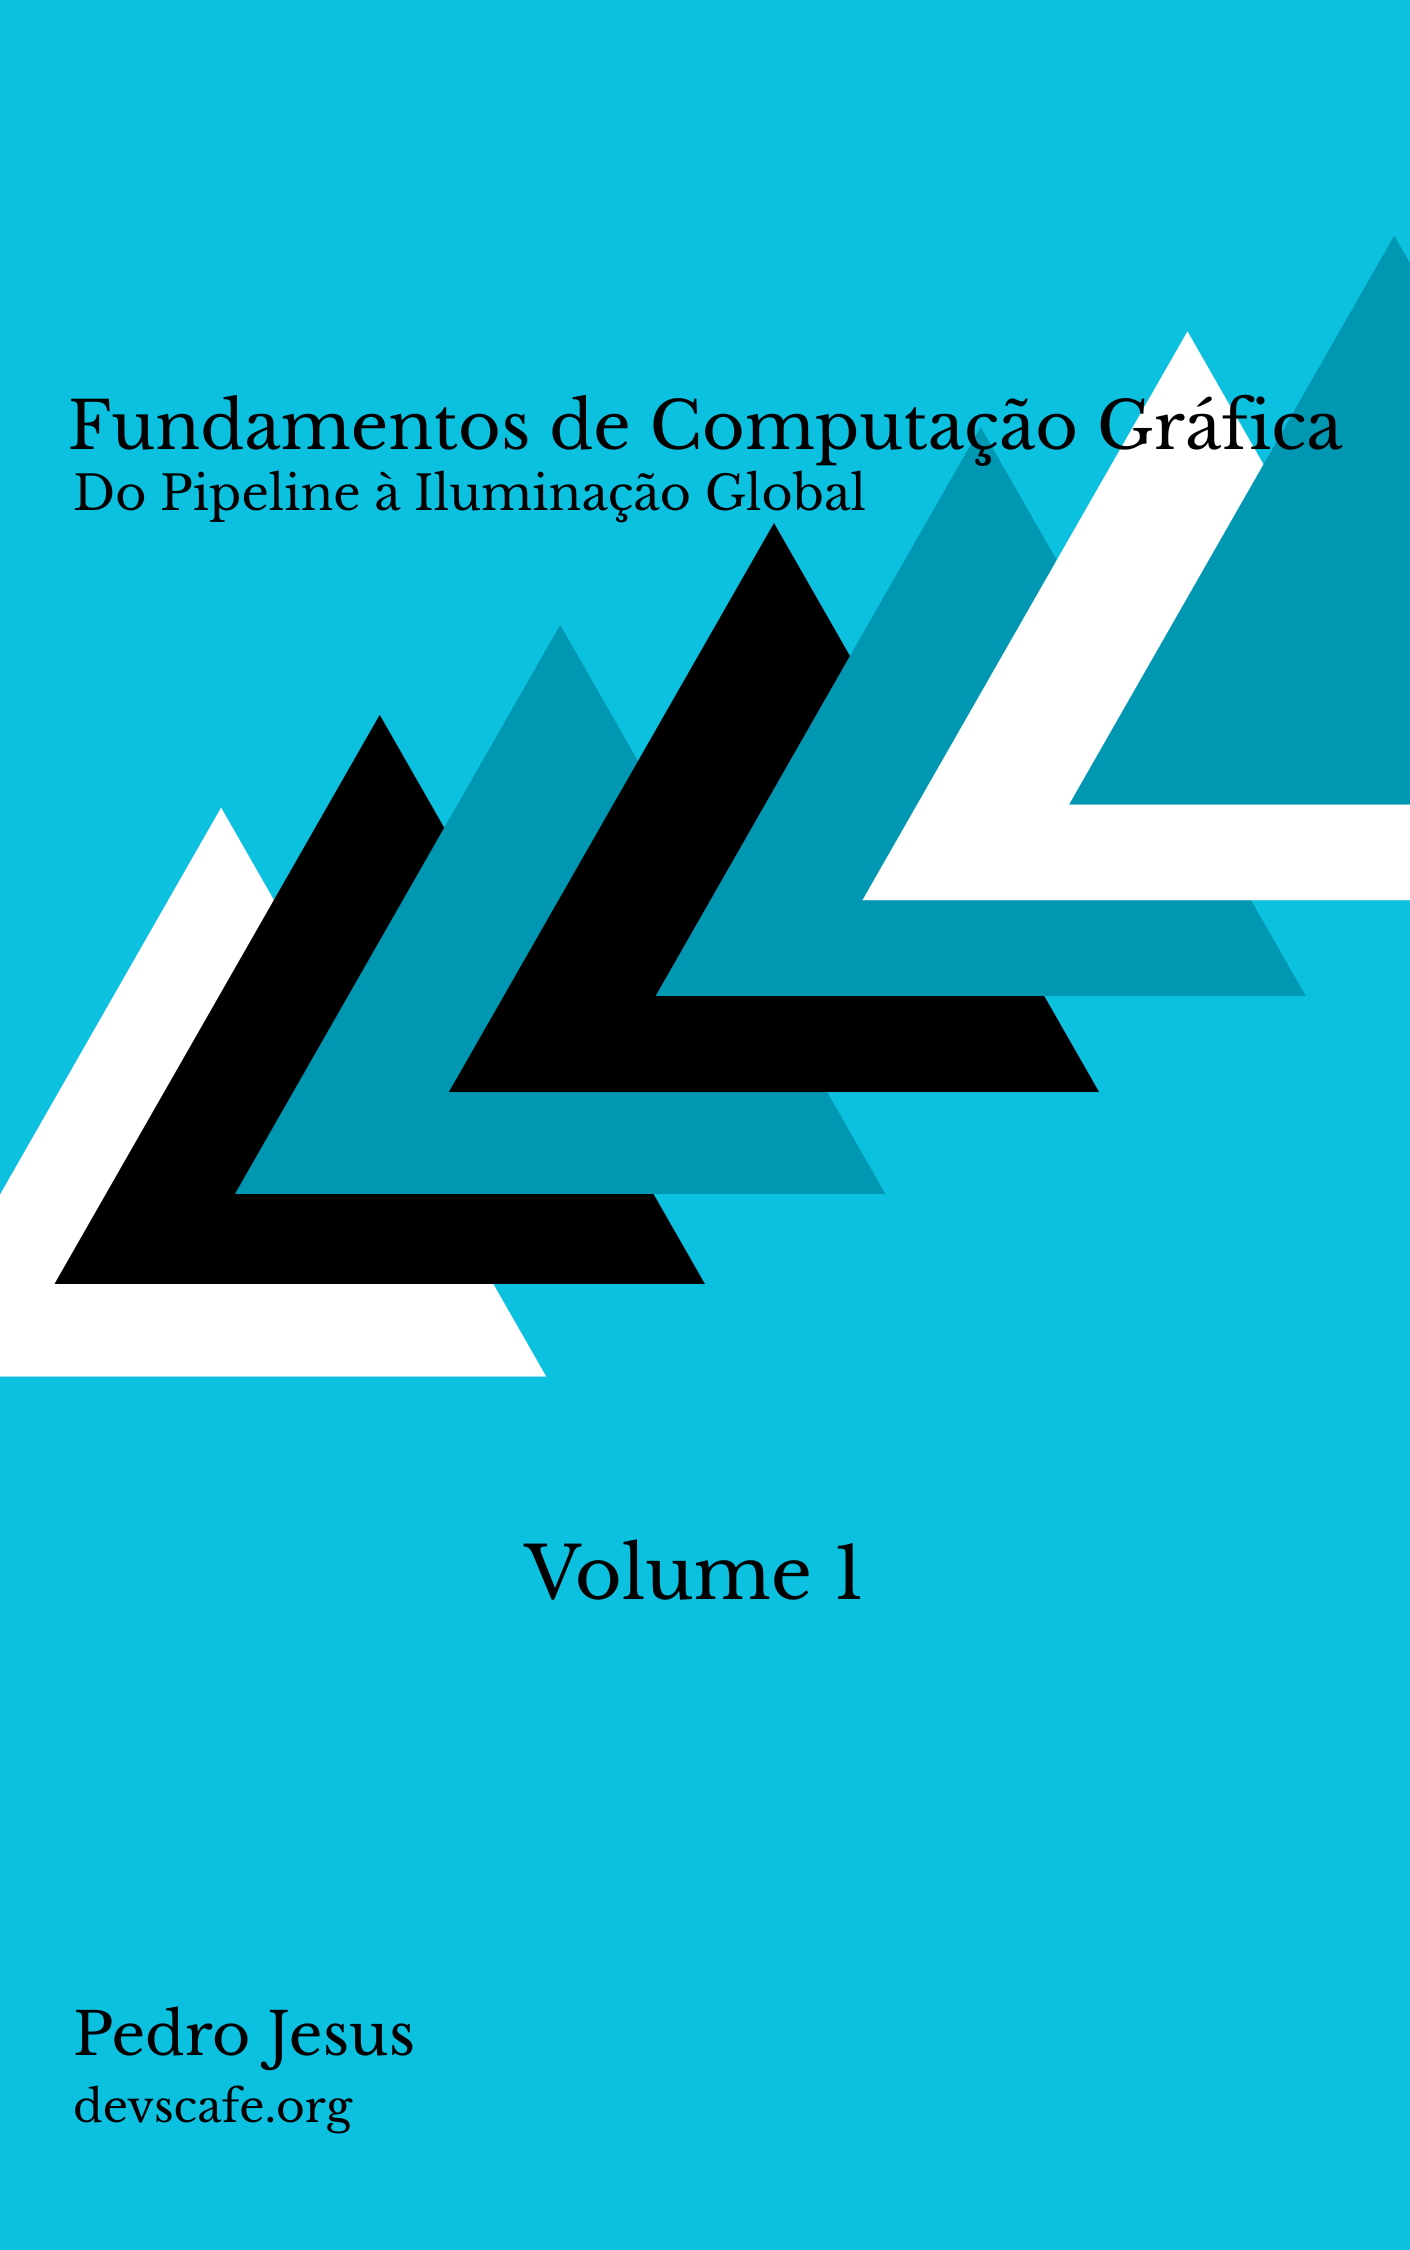
\includegraphics[width=\paperwidth, height=\paperheight, keepaspectratio=false]{assets/cover.png}%
    };
\end{tikzpicture}
\newpage

% === Página de Créditos ===
\thispagestyle{empty}
\vspace*{\fill}
\begin{center}
  \small
  \textbf{Fundamentos de Computação Gráfica (Vol. 1)} \\
  Versão 0.1.0 (Maio de 2026) \\[1.5em]
  \textcite{shirley2021fundamentals} e \textcite{akenine2018realtime} são referências centrais \\
  usadas na elaboração deste material. \\[1.5em]
  \textcopyright\ 2026 Pedro Jesus \\
  Este obra está licenciada sob a \href{https://opensource.org/licenses/MIT}{MIT License}. \\
  Publicado por Dev's Café Biblioteca Didática. \\[1em]
  \url{https://devscafe.org}
\end{center}
\vspace*{\fill}
\newpage

% === Índice ===
\tableofcontents
\newpage

% === Capítulos ===
\chapter{Introdução}

A computação gráfica é a área da ciência da computação que estuda a geração, manipulação e exibição de imagens digitais. O que começou como uma forma simples de desenhar linhas em telas de osciloscópios evoluiu para uma disciplina fundamental que sustenta indústrias multibilionárias. Este volume foca nos alicerces técnicos que permitem transformar dados matemáticos abstratos em experiências visuais ricas. A compreensão profunda desses conceitos permite que desenvolvedores e artistas criem simulações que desafiam a percepção da realidade, unindo matemática, física e percepção humana em um único campo de estudo.

\section{Uma Breve História}

A jornada da computação gráfica moderna começou em 1963 com Ivan Sutherland e seu sistema \textit{Sketchpad}. Este projeto foi revolucionário ao introduzir o uso de uma caneta ótica para manipular objetos geométricos diretamente na tela, estabelecendo os conceitos de interface gráfica e hierarquia de objetos. Sutherland demonstrou que computadores poderiam ser usados para muito mais do que apenas cálculos numéricos puros, abrindo as portas para o design assistido por computador (CAD) e para a manipulação visual interativa.

Nas décadas de 1970 e 1980, a área viu um crescimento explosivo. A fundação do SIGGRAPH (\textit{Special Interest Group on Computer Graphics and Interactive Techniques}) em 1974 criou o fórum principal para a publicação de algoritmos que usamos até hoje. Em 1975, \textcite{phong1975illumination} introduziu um modelo de iluminação que permitiu superfícies mais realistas com brilhos especulares, resolvendo problemas de descontinuidade visual em malhas poligonais. Pouco depois, em 1980, Turner Whitted publicou as bases do \textit{Ray Tracing} recursivo, permitindo reflexões e refrações fidedignas, o que marcou o início da busca pelo fotorrealismo global.

No cinema, a evolução foi marcada por marcos como \textit{Tron} (1982), que usou CGI de forma extensiva, e \textit{Toy Story} (1995), o primeiro longa-metragem totalmente gerado por computador. Recentemente, a revolução do tempo real, impulsionada pelo desenvolvimento de GPUs (\textit{Graphics Processing Units}) cada vez mais poderosas, trouxe gráficos de qualidade cinematográfica para os jogos eletrônicos e simulações interativas. A introdução de técnicas de \textit{Real-Time Ray Tracing} e o uso de inteligência artificial para reconstrução de imagem (como o DLSS e FSR) representam o estado da arte atual.

\section{Aplicações Modernas}

Atualmente, os conceitos que estudaremos neste livro são aplicados em diversas frentes:

\begin{itemize}
    \item \textbf{Jogos Eletrônicos:} Renderização de ambientes complexos a 60 quadros por segundo ou mais, exigindo otimização extrema e uso eficiente do hardware.
    \item \textbf{Cinema e Efeitos Visuais:} Criação de mundos e criaturas que se misturam perfeitamente com filmagens reais, muitas vezes utilizando técnicas de renderização offline que levam horas para processar um único quadro.
    \item \textbf{Visualização Científica e Médica:} Representação de dados complexos, como tomografias computadorizadas e simulações de dinâmica de fluidos, permitindo que pesquisadores identifiquem padrões invisíveis a olho nu.
    \item \textbf{Arquitetura e Engenharia (CAD):} Modelagem e visualização de estruturas antes da construção física, permitindo testes de iluminação natural e ergonomia.
    \item \textbf{Realidade Aumentada e Virtual (AR/VR):} Integração de elementos gráficos com a percepção sensorial do usuário em tempo real, exigindo baixíssima latência para evitar desconforto físico.
    \item \textbf{Treinamento e Simulação:} Simuladores de voo, cirurgias e operação de máquinas pesadas dependem de representações visuais precisas para garantir a transferência de habilidades para o mundo real.
\end{itemize}

\section{Radiometria e Fotometria Introdutórias}

Para entender como a luz interage com as superfícies, precisamos de uma base sólida em radiometria, que é o estudo da medição da radiação eletromagnética, incluindo a luz visível. A fotometria é um campo relacionado, mas que pondera as medições de acordo com a sensibilidade do olho humano.

\begin{itemize}
    \item \textbf{Fluxo Radiante ($\Phi$):} É a energia total emitida, refletida, transmitida ou recebida por unidade de tempo. Sua unidade no SI é o Watt (W).
    \item \textbf{Irradiância ($E$):} Define o fluxo radiante recebido por uma superfície por unidade de área. É expressa em $W/m^2$. A irradiância é fundamental para calcular quanta energia atinge um ponto no espaço.
    \item \textbf{Radiância ($L$):} É a medida mais importante para a computação gráfica. Ela descreve a quantidade de luz que passa através ou é emitida por uma superfície em uma direção específica, por unidade de área projetada e por unidade de ângulo sólido. Sua unidade é $W/(m^2 \cdot sr)$.
\end{itemize}

\begin{formula}{Definições Radiométricas}
    A relação entre irradiância e radiância é dada pela integral sobre o hemisfério $\Omega$:
    \[ E = \int_\Omega L(\omega) \cos \theta \, d\omega \]
    Onde $\theta$ é o ângulo entre a direção da luz $\omega$ e a normal da superfície.
\end{formula}

\section{A Equação de Renderização}

O problema central da computação gráfica é resolver a equação de renderização, introduzida por \textcite{kajiya1986rendering}. Esta equação integral descreve o equilíbrio de luz em uma cena e é a base para todos os algoritmos de renderização fisicamente correta (PBR).

A equação é expressa como:
\[ L_o(\mathbf{x}, \omega_o) = L_e(\mathbf{x}, \omega_o) + \int_\Omega f_r(\mathbf{x}, \omega_i, \omega_o) L_i(\mathbf{x}, \omega_i)(\hat{n}\cdot\omega_i) d\omega_i \]

Cada termo possui um significado físico preciso:
\begin{enumerate}
    \item $L_o(\mathbf{x}, \omega_o)$: A radiância de saída do ponto $\mathbf{x}$ na direção $\omega_o$. É o que a câmera ou o olho percebe.
    \item $L_e(\mathbf{x}, \omega_o)$: A radiância emitida pelo ponto $\mathbf{x}$ na direção $\omega_o$. Este termo é diferente de zero apenas se a superfície for uma fonte de luz.
    \item $\int_\Omega \dots d\omega_i$: Representa a soma de toda a luz incidente vinda de todas as direções no hemisfério acima do ponto $\mathbf{x}$.
    \item $f_r(\mathbf{x}, \omega_i, \omega_o)$: A Função de Distribuição de Refletância Bidirecional (BRDF). Ela define como a luz incidente de uma direção $\omega_i$ é espalhada para a direção de saída $\omega_o$.
    \item $L_i(\mathbf{x}, \omega_i)$: A radiância incidente vinda da direção $\omega_i$.
    \item $(\hat{n}\cdot\omega_i)$: O termo de cosseno que representa a atenuação da luz devido à inclinação da superfície em relação à fonte de luz (Lei de Lambert).
\end{enumerate}

\begin{aviso}
    Resolver esta integral é computacionalmente proibitivo de forma exata. Por isso, usamos métodos numéricos como o Método de Monte Carlo para aproximar o resultado em algoritmos de \textit{Path Tracing}.
\end{aviso}

\section{Hardware: CPU vs GPU}

A arquitetura dos computadores modernos reflete as demandas da computação gráfica. Enquanto a CPU é projetada para execução sequencial complexa, a GPU é uma máquina de paralelismo massivo.

\begin{itemize}
    \item \textbf{CPU (Central Processing Unit):} Focada em baixa latência e controle de fluxo complexo. Possui poucos núcleos, mas cada um é extremamente poderoso e capaz de realizar operações lógicas avançadas com grandes caches.
    \item \textbf{GPU (Graphics Processing Unit):} Focada em alto rendimento (\textit{throughput}). Possui milhares de pequenos núcleos que executam a mesma instrução sobre diferentes conjuntos de dados simultaneamente (SIMD - \textit{Single Instruction, Multiple Data}).
\end{itemize}

O modelo de execução das GPUs é frequentemente descrito como SIMT (\textit{Single Instruction, Multiple Threads}). Isso permite que a GPU processe milhões de vértices e pixels em paralelo, o que é perfeito para tarefas gráficas onde o mesmo cálculo de cor ou transformação é aplicado a grandes quantidades de dados independentes. Os \textit{Shader Cores} são as unidades fundamentais de processamento que executam os programas programáveis do pipeline.

\section{O Pipeline de Renderização}

Transformar uma cena 3D composta por coordenadas matemáticas em um conjunto de pixels na tela exige uma sequência de transformações conhecida como \textit{Pipeline de Renderização}. Este processo pode ser visualizado como uma linha de produção industrial.

\begin{center}
\begin{tikzpicture}[
    node distance=1.5cm,
    block/.style={rectangle, draw, fill=blue!10, text width=3cm, text centered, rounded corners, minimum height=1cm},
    arrow/.style={thick,->,>=stealth}
]
    \node (geo) [block] {Geometria (Vértices)};
    \node (trans) [block, below of=geo] {Transformações (Espaços)};
    \node (rast) [block, below of=trans] {Rasterização (Fragmentos)};
    \node (shading) [block, below of=rast] {Shading (Pixels)};
    \node (display) [block, below of=shading, fill=green!10] {Exibição (Tela)};

    \draw [arrow] (geo) -- (trans);
    \draw [arrow] (trans) -- (rast);
    \draw [arrow] (rast) -- (shading);
    \draw [arrow] (shading) -- (display);
\end{tikzpicture}
\end{center}

De forma detalhada, o processo segue estas etapas fundamentais descritas por \textcite{akenine2018realtime}:
\begin{enumerate}
    \item \textbf{Processamento de Vértices:} Aplicação de matrizes de transformação para posicionar objetos no mundo e projetá-los para a câmera.
    \item \textbf{Montagem de Primitivas:} Agrupamento de vértices em triângulos ou linhas.
    \item \textbf{Rasterização:} Conversão da geometria contínua em fragmentos discretos. É aqui que determinamos quais pixels do monitor são cobertos por cada triângulo.
    \item \textbf{Processamento de Fragmentos:} Cálculo da cor final, aplicação de texturas e iluminação.
    \item \textbf{Operações de Per-Sample:} Testes de profundidade (z-buffer), stencil e mistura de cores (blending).
\end{enumerate}

\section{O Que Você Vai Aprender}

Este volume foca no "como" e no "porquê". Não ensinaremos a usar uma ferramenta específica como Blender ou Unity, mas sim a matemática e os algoritmos que estas ferramentas utilizam. O objetivo é que, ao final da leitura, você consiga implementar seu próprio motor de renderização ou escrever \textit{shaders} complexos com total domínio técnico. Exploraremos desde a geometria básica até as sutilezas da luz e sombra, preparando-o para os desafios reais do desenvolvimento de software gráfico de alto desempenho.

\begin{aviso}
    Este volume não cobre animação de personagens, simulação física avançada ou técnicas de inteligência artificial aplicadas a gráficos. Esses temas serão abordados em volumes futuros.
\end{aviso}

\section{Pré-requisitos}

Para aproveitar este conteúdo, é essencial ter uma base sólida em:
\begin{itemize}
    \item \textbf{Álgebra Linear:} Vetores, matrizes, produtos escalares e vetoriais, e transformações espaciais são a linguagem da computação gráfica.
    \item \textbf{Cálculo:} Entender derivadas e integrais é vital para compreender a equação de renderização e modelos de iluminação avançados.
    \item \textbf{Programação:} Familiaridade com linguagens de baixo nível ou C-like (C++, C\#, Java ou GLSL) ajudará na compreensão dos algoritmos e na implementação prática dos projetos.
\end{itemize}

\begin{dica}
    Não se sinta intimidado pela matemática. Como afirma \textcite{shirley2021fundamentals}, a computação gráfica é visual. Sempre que encontrar uma fórmula difícil, tente desenhá-la. A intuição geométrica é sua melhor aliada. A prática constante de converter fórmulas em código é o que solidifica o conhecimento.
\end{dica}

\section*{Exercícios}

\begin{exercicio}{Fundamentos Históricos}
    Pesquise sobre o sistema \textit{Sketchpad} de Ivan Sutherland. Quais conceitos introduzidos por ele ainda são usados na computação gráfica moderna? Como a interação direta mudou o paradigma da computação na época?
\end{exercicio}

\begin{exercicio}{Tempo Real vs Offline}
    Explique a diferença fundamental entre renderização em tempo real (\textit{Real-Time Rendering}) e renderização \textit{Offline}. Cite exemplos de hardware e software típicos para cada uma e discuta o compromisso entre qualidade visual e velocidade.
\end{exercicio}

\begin{exercicio}{Importância da Matemática}
    Por que a computação gráfica depende tanto da Álgebra Linear? Dê um exemplo prático de como uma rotação de um objeto 3D é representada matematicamente e como isso é processado pela GPU.
\end{exercicio}

\begin{exercicio}{A Equação de Renderização}
    Como o trabalho de \textcite{kajiya1986rendering} mudou a forma como pensamos sobre a luz em ambientes digitais? Explique o conceito de iluminamento global que esta equação tenta formalizar.
\end{exercicio}

\begin{exercicio}{Aplicações Diversas}
    Cite três áreas fora do entretenimento onde a computação gráfica é essencial e descreva o benefício gerado. Como a visualização científica pode auxiliar na descoberta de novos medicamentos?
\end{exercicio}

\begin{exercicio}{Unidades Radiométricas}
    Diferencie Fluxo Radiante, Irradiância e Radiância. Se uma fonte de luz emite 100 Watts uniformemente em todas as direções, qual será a irradiância em uma esfera de raio 2 metros centrada na fonte?
\end{exercicio}

\begin{exercicio}{Arquitetura de Hardware}
    Explique os conceitos de SIMD e SIMT. Por que um processador com centenas de núcleos simples (GPU) é mais eficiente para renderização do que um processador com poucos núcleos complexos (CPU)?
\end{exercicio}

\begin{exercicio}{O Papel da BRDF}
    Na equação de renderização, qual é a função do termo $f_r$? Como você descreveria a BRDF de um espelho perfeito comparada a uma superfície de gesso fosco?
\end{exercicio}

\chapter{Matemática Essencial}

A computação gráfica é, em sua essência, matemática aplicada e visualizada. Para posicionar objetos em uma cena virtual, simular o comportamento da luz e projetar um mundo tridimensional em uma tela bidimensional, precisamos de um conjunto de ferramentas robustas da álgebra linear e geometria analítica. Neste capítulo, construiremos os alicerces necessários para entender como os pixels ganham vida através de equações.

\section{Vetores}

Um vetor é uma entidade matemática que possui tanto magnitude quanto direção. Geometricamente, podemos visualizá-lo como uma seta no espaço. Algebricamente, em $\mathbb{R}^3$, representamos um vetor $\mathbf{v}$ como uma tripla de números reais:

\begin{equation}
    \mathbf{v} = \begin{bmatrix} v_x \\ v_y \\ v_z \end{bmatrix}
\end{equation}

\subsection{Operações Básicas}

Dadas dois vetores $\mathbf{u} = (u_x, u_y, u_z)$ e $\mathbf{v} = (v_x, v_y, v_z)$, e um escalar $s$:

\begin{itemize}
    \item \textbf{Soma e Diferença:} $\mathbf{u} \pm \mathbf{v} = (u_x \pm v_x, u_y \pm v_y, u_z \pm v_z)$. Geometricamente, a soma segue a regra do paralelogramo.
    \item \textbf{Multiplicação por Escalar:} $s\mathbf{v} = (sv_x, sv_y, sv_z)$. Altera a magnitude do vetor e inverte sua direção se $s < 0$.
    \item \textbf{Magnitude (Norma):} A distância euclidiana da origem à extremidade do vetor:
    \begin{formula}{Magnitude}
        \|\mathbf{v}\| = \sqrt{v_x^2 + v_y^2 + v_z^2}
    \end{formula}
    \item \textbf{Normalização:} Transformar um vetor em um \textbf{vetor unitário} ($\|\mathbf{v}\| = 1$) mantendo sua direção:
    \begin{equation}
        \hat{\mathbf{v}} = \frac{\mathbf{v}}{\|\mathbf{v}\|}
    \end{equation}
\end{itemize}

\section{Produto Escalar (Dot Product)}

O produto escalar entre dois vetores $\mathbf{a}$ e $\mathbf{b}$ resulta em um escalar e é definido como:

\begin{formula}{Produto Escalar}
    \mathbf{a} \cdot \mathbf{b} = a_x b_x + a_y b_y + a_z b_z = \|\mathbf{a}\| \|\mathbf{b}\| \cos\theta
\end{formula}

Onde $\theta$ é o ângulo entre os vetores.

\subsection{Propriedades e Uso}

\begin{itemize}
    \item Se $\mathbf{a} \cdot \mathbf{b} > 0$, o ângulo entre eles é agudo.
    \item Se $\mathbf{a} \cdot \mathbf{b} = 0$, os vetores são \textbf{ortogonais}.
    \item Se $\mathbf{a} \cdot \mathbf{b} < 0$, o ângulo é obtuso.
\end{itemize}

Na computação gráfica, o produto escalar é o coração dos cálculos de iluminação. Por exemplo, no modelo de reflexão difusa de Lambert, a intensidade da luz em um ponto da superfície é proporcional ao produto escalar entre a normal da superfície $\hat{\mathbf{n}}$ e a direção da luz $\hat{\mathbf{l}}$, ambos unitários. Isso nos dá o cosseno do ângulo de incidência.

\section{Produto Vetorial (Cross Product)}

O produto vetorial $\mathbf{a} \times \mathbf{b}$ só é definido em $\mathbb{R}^3$ e resulta em um vetor perpendicular a ambos.

\begin{formula}{Produto Vetorial}
    \mathbf{a} \times \mathbf{b} = \begin{vmatrix}
    \mathbf{i} & \mathbf{j} & \mathbf{k} \\
    a_x & a_y & a_z \\
    b_x & b_y & b_z
    \end{vmatrix} = \begin{bmatrix} a_y b_z - a_z b_y \\ a_z b_x - a_x b_z \\ a_x b_y - a_y b_x \end{bmatrix}
\end{formula}

\subsection{Propriedades}

\begin{itemize}
    \item \textbf{Anti-comutatividade:} $\mathbf{a} \times \mathbf{b} = -(\mathbf{b} \times \mathbf{a})$.
    \item \textbf{Magnitude:} $\|\mathbf{a} \times \mathbf{b}\| = \|\mathbf{a}\| \|\mathbf{b}\| \sin\theta$, que corresponde à área do paralelogramo formado pelos dois vetores.
    \item \textbf{Normais de Superfície:} Se temos dois vetores tangentes a um triângulo, seu produto vetorial nos dá a normal da face.
\end{itemize}

\section{Matrizes}

Uma matriz $m \times n$ organiza dados em $m$ linhas e $n$ colunas. Em CG, usamos principalmente matrizes $3 \times 3$ e $4 \times 4$.

\subsection{Operações e Propriedades}

\begin{itemize}
    \item \textbf{Multiplicação de Matrizes:} O elemento $c_{ij}$ da matriz resultante $C = AB$ é o produto escalar da linha $i$ de $A$ pela coluna $j$ de $B$.
    \item \textbf{Não-comutatividade:} Em geral, $AB \neq BA$. A ordem das transformações importa!
    \item \textbf{Transposta:} $A^T$ é obtida trocando linhas por colunas.
    \item \textbf{Identidade ($I$):} Matriz quadrada com 1 na diagonal principal e 0 no restante. $AI = IA = A$.
\end{itemize}

\subsection{Determinante e Inversa}

O determinante de uma matriz $3 \times 3$ pode ser calculado pela regra de Sarrus. Geometricamente, o determinante representa o fator de escala de volume da transformação. Se $\det(A) = 0$, a matriz é \textbf{singular} e não possui inversa.

A inversa $A^{-1}$ desfaz a transformação de $A$: $AA^{-1} = I$. Para matrizes ortogonais (como matrizes de rotação pura), a inversa é simplesmente a transposta ($A^{-1} = A^T$), o que é uma otimização comum em motores de jogo.

\section{Transformações Geométricas}

Transformar um objeto significa alterar a posição de seus vértices.

\subsection{Coordenadas Homogêneas}

Uma matriz $3 \times 3$ pode representar escala e rotação, mas não pode representar translação de forma linear. Para unificar todas as transformações (incluindo projeção perspectiva), adicionamos uma quarta componente $w$ ao vetor $[x, y, z, w]^T$.

\begin{itemize}
    \item \textbf{Ponto:} Usamos $w=1$. Quando multiplicado por uma matriz de translação, a posição muda.
    \item \textbf{Vetor (Direção):} Usamos $w=0$. Vetores de direção não têm posição, logo são imunes à translação.
\end{itemize}

Ao final do pipeline, realizamos a \textbf{divisão perspectiva}: dividimos $x, y, z$ por $w$ para retornar ao espaço 3D real.

\subsection{Translação}

Dada uma translação $\mathbf{t} = (t_x, t_y, t_z)$:

\begin{equation}
    T(\mathbf{t}) = \begin{bmatrix}
    1 & 0 & 0 & t_x \\
    0 & 1 & 0 & t_y \\
    0 & 0 & 1 & t_z \\
    0 & 0 & 0 & 1
    \end{bmatrix}
\end{equation}

\subsection{Escala}

A escala por fatores $s_x, s_y, s_z$ é dada por:

\begin{equation}
    S(s_x, s_y, s_z) = \begin{bmatrix}
    s_x & 0 & 0 & 0 \\
    0 & s_y & 0 & 0 \\
    0 & 0 & s_z & 0 \\
    0 & 0 & 0 & 1
    \end{bmatrix}
\end{equation}

Se $s_x = s_y = s_z$, temos uma escala uniforme.

\subsection{Rotação}

As matrizes de rotação em torno dos eixos principais são derivadas da trigonometria básica no plano 2D. Por exemplo, em torno de $Z$, as coordenadas $x$ e $y$ mudam enquanto $z$ permanece constante:

\begin{equation}
    R_z(\theta) = \begin{bmatrix}
    \cos\theta & -\sin\theta & 0 & 0 \\
    \sin\theta & \cos\theta & 0 & 0 \\
    0 & 0 & 1 & 0 \\
    0 & 0 & 0 & 1
    \end{bmatrix}
\end{equation}

Para os outros eixos:

\begin{equation}
    R_x(\theta) = \begin{bmatrix}
    1 & 0 & 0 & 0 \\
    0 & \cos\theta & -\sin\theta & 0 \\
    0 & \sin\theta & \cos\theta & 0 \\
    0 & 0 & 0 & 1
    \end{bmatrix}, \quad
    R_y(\theta) = \begin{bmatrix}
    \cos\theta & 0 & \sin\theta & 0 \\
    0 & 1 & 0 & 0 \\
    -\sin\theta & 0 & \cos\theta & 0 \\
    0 & 0 & 0 & 1
    \end{bmatrix}
\end{equation}

Para rotação em torno de um eixo arbitrário $\hat{\mathbf{u}}$, usamos a \textbf{Fórmula de Rodrigues}:
\begin{formula}{Fórmula de Rodrigues}
    \mathbf{v}_{rot} = \mathbf{v}\cos\theta + (\hat{\mathbf{u}} \times \mathbf{v})\sin\theta + \hat{\mathbf{u}}(\hat{\mathbf{u}} \cdot \mathbf{v})(1 - \cos\theta)
\end{formula}

\section{Composição de Transformações}

Para aplicar várias transformações a um objeto, multiplicamos as matrizes. A ordem é crucial. Usando vetores coluna, a aplicação ocorre da direita para a esquerda. Para transladar, rotacionar e escalar um objeto (nesta ordem lógica de "espaço local"):

\begin{equation}
    M_{final} = T \cdot R \cdot S
\end{equation}

Isso significa que o vértice $\mathbf{v}$ será processado como $\mathbf{v}' = T(R(S\mathbf{v}))$. Se trocarmos a ordem de $T$ e $R$, o objeto rotacionará em torno da origem do mundo, não em torno do seu próprio centro.

\section{Mudança de Base e Normais}

Uma matriz de mudança de base transforma coordenadas de um sistema de eixos para outro. Se tivermos eixos ortonormais $\mathbf{u}, \mathbf{v}, \mathbf{w}$, a matriz que transforma do espaço local para o global é:

\begin{equation}
    M = \begin{bmatrix} u_x & v_x & w_x & 0 \\ u_y & v_y & w_y & 0 \\ u_z & v_z & w_z & 0 \\ 0 & 0 & 0 & 1 \end{bmatrix}
\end{equation}

\begin{aviso}
    Normais de superfície não podem ser transformadas pela mesma matriz $M$ que transforma os pontos, especialmente se houver escala não-uniforme. Para manter a normal perpendicular à superfície, devemos usar a \textbf{transposta da inversa} de $M$: $N = (M^{-1})^T$.
\end{aviso}

\section{Quaternions}

Embora matrizes de rotação sejam eficientes, elas sofrem de dois problemas: \textbf{Gimbal Lock} (perda de um grau de liberdade ao alinhar dois eixos de rotação) e dificuldade em interpolar entre duas orientações.

Os quaternions resolvem isso. Um quaternion unitário representa uma rotação no espaço 4D:
\begin{equation}
    \mathbf{q} = w + xi + yj + zk = (\cos\frac{\theta}{2}, \hat{\mathbf{u}}\sin\frac{\theta}{2})
\end{equation}

Onde $\hat{\mathbf{u}}$ é o eixo e $\theta$ o ângulo.

\subsection{Operações e Vantagens}

\begin{itemize}
    \item \textbf{Multiplicação:} Representa a combinação de duas rotações. É mais barata que a multiplicação de matrizes 4x4.
    \item \textbf{Conjugado:} $\mathbf{q}^* = w - xi - yj - zk$. Representa a rotação inversa.
    \item \textbf{SLERP (Spherical Linear Interpolation):} Permite interpolar suavemente entre duas rotações $\mathbf{q}_0$ e $\mathbf{q}_1$ com velocidade angular constante.
\end{itemize}

\section*{Exercícios}

\begin{enumerate}
    \item Dados os vetores $\mathbf{a} = (1, 2, 3)$ e $\mathbf{b} = (4, -5, 6)$, calcule $\mathbf{a} \cdot \mathbf{b}$ e $\mathbf{a} \times \mathbf{b}$.
    \item Demonstre que para qualquer vetor unitário $\hat{\mathbf{v}}$, o produto escalar $\hat{\mathbf{v}} \cdot \hat{\mathbf{v}} = 1$.
    \item Construa a matriz de transformação 4x4 que primeiro escala um objeto por 2 em todos os eixos e depois o translada para a posição $(10, 5, 0)$.
    \item Explique, com um diagrama descrito, por que a ordem $T \cdot R$ é diferente de $R \cdot T$.
    \item Deduza a matriz de rotação $R_y(\theta)$ a partir de um círculo unitário no plano $XZ$.
    \item Dada a matriz de modelo $M$ que inclui uma escala de $(1, 2, 1)$, calcule a matriz necessária para transformar as normais corretamente.
\end{enumerate}

\chapter{O Pipeline de Renderização}

O pipeline de renderização é o modelo conceitual e prático que descreve os passos necessários para transformar uma cena tridimensional em uma imagem bidimensional. Este processo é uma linha de montagem altamente otimizada onde dados de geometria entram em uma ponta e cores de pixels saem na outra. Como detalhado por \textcite{akenine2018realtime}, o pipeline moderno é dividido em estágios funcionais, alguns fixos e outros totalmente programáveis através de \textit{shaders}. A evolução das GPUs permitiu que partes que antes eram fixas agora sejam controladas pelo desenvolvedor, oferecendo uma flexibilidade sem precedentes para a criação de efeitos visuais complexos. O entendimento deste fluxo é vital para qualquer programador gráfico, pois permite identificar gargalos de performance e implementar técnicas avançadas de renderização.

Transformar números em imagens exige uma série de transformações matemáticas rigorosas. Cada estágio do pipeline resolve um problema específico: como posicionar objetos, como simular a visão de uma câmera, como cortar o que não é visível e como colorir cada ponto de forma realista. Ao longo deste capítulo, exploraremos cada um desses passos em detalhes técnicos, fornecendo a base para a compreensão de como os motores de jogos modernos operam. A arquitetura de hardware das GPUs foi desenhada especificamente para acelerar estes estágios, permitindo o processamento de milhões de polígonos por quadro.

\section{Visão Geral do Pipeline}

Podemos visualizar o pipeline como uma sequência de quatro macro-estágios principais, cada um com responsabilidades específicas e formas distintas de processamento. A eficiência do sistema depende de quão bem esses estágios são balanceados, evitando que um estágio se torne um gargalo para os outros. Cada estágio pode ser visto como uma camada de abstração que aproxima os dados geométricos puros da representação final em pixels.

\begin{table}[H]
\centering
\begin{tabularx}{\textwidth}{l|X}
\toprule
\textbf{Estágio} & \textbf{Descrição Principal} \\
\midrule
Aplicação & Lógica de CPU, detecção de colisão, culling grosseiro, animação de sistemas e submissão de dados de geometria para a GPU através de comandos da API. \\
Geometria & Transformações de espaços (Model, View, Projection), clipping, montagem de primitivas, iluminação por vértice e mapeamento de viewport. \\
Rasterização & Conversão de primitivas geométricas (triângulos) em fragmentos discretos, determinando a cobertura de pixels e interpolando atributos. \\
Fragmento & Execução de \textit{pixel shaders}, aplicação de texturas, cálculos de iluminação por fragmento e testes finais de visibilidade e mistura de cores. \\
\bottomrule
\end{tabularx}
\caption{Os macro-estágios do pipeline de renderização.}
\end{table}

\section{Estágio de Aplicação}

Este estágio ocorre inteiramente na CPU e é o ponto de partida de qualquer aplicação gráfica. Sua principal função é preparar a cena de tal forma que a GPU receba apenas o necessário para renderizar o quadro atual. Como a CPU lida bem com lógica complexa, ramificações imprevisíveis e acesso aleatório à memória, ela é ideal para gerenciar o estado global da aplicação e a interação com o usuário.

As tarefas típicas incluem:

\begin{itemize}
    \item \textbf{Culling de Frustum:} Este processo identifica quais objetos estão total ou parcialmente dentro do volume de visão da câmera. Objetos que estão completamente fora não são enviados para a GPU, economizando largura de banda e ciclos de processamento preciosos. É uma otimização de nível superior que evita sobrecarregar o restante do pipeline.
    \item \textbf{Hierarquia de Cena:} Gerenciar o posicionamento relativo de objetos através de grafos de cena. Por exemplo, se um carro se move, todas as suas partes internas e o motorista devem se mover proporcionalmente sem que cada vértice precise ser atualizado manualmente pelo programador. A CPU calcula as matrizes de mundo acumuladas.
    \item \textbf{Sistemas de Partículas e Física:} Embora algumas simulações possam rodar na GPU via \textit{compute shaders}, muitas vezes a lógica de jogo, detecção de colisão entre objetos e interações físicas simples são resolvidas aqui.
    \item \textbf{Draw Calls:} A submissão de comandos para a API gráfica (como OpenGL, Vulkan ou DirectX). Cada \textit{draw call} possui um custo de processamento significativo no driver da placa de vídeo, portanto, organizar a geometria em blocos eficientes ou usar \textit{texture atlases} é uma técnica de otimização crucial.
\end{itemize}

O gargalo neste estágio costuma ser a comunicação entre CPU e GPU, conhecida como "overhead de driver". Por isso, técnicas modernas como o \textit{instancing} permitem desenhar milhares de cópias do mesmo objeto com uma única chamada de comando, reduzindo drasticamente a carga na CPU. Além disso, a CPU é responsável por gerenciar a memória de vídeo, decidindo quando descartar texturas ou carregar novos modelos.

\section{Estágio de Geometria}

Este estágio é onde a fundamentação matemática é aplicada em larga escala para transformar coordenadas abstratas em posições na tela. Ele opera principalmente sobre vértices e primitivas, sendo altamente paralelizável nas GPUs modernas através do \textit{Vertex Shader} e, opcionalmente, \textit{Geometry} e \textit{Tessellation Shaders}.

\subsection{Transformação de Modelo (Model Transform)}

O primeiro passo é levar os vértices do \textbf{Object Space}, onde cada modelo é definido em seu próprio sistema de coordenadas local, para o \textbf{World Space}. Isso é feito multiplicando cada vértice pela matriz de modelo $M$. Esta matriz contém as informações de translação, rotação e escala do objeto na cena global. Sem essa etapa, todos os objetos da cena estariam amontoados na origem do mundo, compartilhando o mesmo espaço físico. A matriz $M$ é tipicamente o produto de várias matrizes de transformação elementares.

\subsection{Transformação de Visualização (View Transform)}

A transformação de visualização move o mundo inteiro para que a câmera se torne o centro do universo. No \textbf{View Space} (ou \textit{Camera Space}), a câmera está na origem $(0,0,0)$ e olha para uma direção padrão, geralmente o eixo $-Z$ em sistemas \textit{right-handed}. Isso simplifica imensamente os cálculos de projeção subsequentes, pois a profundidade passa a ser simplesmente a coordenada $z$.

Para derivar a matriz de visualização $V$, usamos a função \textit{LookAt}. Dados a posição da câmera $\mathbf{e}$, o ponto alvo $\mathbf{t}$ e um vetor de referência para cima $\mathbf{up}_{world}$, construímos um sistema de coordenadas ortonormal que define a orientação da câmera:

\begin{enumerate}
    \item $\mathbf{f} = \text{normalize}(\mathbf{t} - \mathbf{e})$ (vetor para frente)
    \item $\mathbf{r} = \text{normalize}(\mathbf{f} \times \mathbf{up}_{world})$ (vetor para a direita)
    \item $\mathbf{u} = \mathbf{r} \times \mathbf{f}$ (vetor para cima corrigido)
\end{enumerate}

\begin{formula}{Matriz LookAt}
    A matriz de visualização completa combina a translação da câmera para a origem com a rotação para alinhar os eixos do mundo com os da câmera. Ela é dada por:
    \[ V = \begin{bmatrix} r_x & r_y & r_z & -\mathbf{r}\cdot\mathbf{e} \\ u_x & u_y & u_z & -\mathbf{u}\cdot\mathbf{e} \\ -f_x & -f_y & -f_z & \mathbf{f}\cdot\mathbf{e} \\ 0 & 0 & 0 & 1 \end{bmatrix} \]
    Onde $\mathbf{r}, \mathbf{u}$ e $\mathbf{f}$ são os eixos unitários da câmera e $\mathbf{e}$ é sua posição no mundo. Esta matriz é efetivamente a inversa da matriz que posicionaria uma "câmera objeto" na cena. O uso do produto escalar nos termos da quarta coluna é uma forma computacionalmente eficiente de representar a translação inversa no espaço rotacionado.
\end{formula}

\subsection{Projeção Perspectiva}

A projeção mapeia o volume de visualização da câmera (o \textit{frustum}) para um cubo unitário. Na projeção perspectiva, o efeito de encurtamento faz com que objetos distantes pareçam menores, imitando o comportamento das lentes ópticas e do olho humano. Esta transformação não é linear no espaço 3D, mas torna-se linear no espaço projetivo 4D.

A derivação começa com a semelhança de triângulos no espaço de visualização. Para um ponto $P(x, y, z)$, sua projeção em um plano a uma distância $n$ (near) é dada por:
\[ x_{proj} = \frac{n \cdot x}{-z}, \quad y_{proj} = \frac{n \cdot y}{-z} \]

Para formalizar isso em uma matriz 4x4 que mapeia o volume definido por $l$ (left), $r$ (right), $b$ (bottom), $t$ (top), $n$ (near) e $f$ (far), chegamos à matriz de projeção perspectiva padrão. O uso de coordenadas homogêneas permite que a divisão pelo $z$ seja adiada para uma etapa posterior de hardware, garantindo que as operações de interpolação ocorram corretamente.

\begin{formula}{Matriz de Projeção Perspectiva}
    A matriz que mapeia o frustum para o Clip Space, preservando a profundidade de forma não-linear para otimizar a precisão do z-buffer, é:
    \[ P = \begin{bmatrix} \frac{2n}{r-l} & 0 & \frac{r+l}{r-l} & 0 \\ 0 & \frac{2n}{t-b} & \frac{t+b}{t-b} & 0 \\ 0 & 0 & -\frac{f+n}{f-n} & -\frac{2fn}{f-n} \\ 0 & 0 & -1 & 0 \end{bmatrix} \]
    Se usarmos o Campo de Visão Vertical ($fov_y$) e a Razão de Aspecto ($a = w/h$), assumindo simetria:
    \[ P = \begin{bmatrix} \frac{1}{a \cdot \tan(fov_y/2)} & 0 & 0 & 0 \\ 0 & \frac{1}{\tan(fov_y/2)} & 0 & 0 \\ 0 & 0 & -\frac{f+n}{f-n} & -\frac{2fn}{f-n} \\ 0 & 0 & -1 & 0 \end{bmatrix} \]
\end{formula}

\subsection{Projeção Ortográfica}

Na projeção ortográfica, o volume de visualização é uma caixa retangular. As linhas de projeção são paralelas, o que significa que o tamanho de um objeto não muda com a distância. É a base para desenhos técnicos, interfaces de usuário (UI) e jogos isométricos. Ela é útil quando a preservação de medidas e proporções paralelas é mais importante do que o realismo da profundidade.

\begin{formula}{Matriz de Projeção Ortográfica}
    Diferente da perspectiva, esta matriz é uma transformação linear pura de escala e translação, mapeando o volume da caixa para o cubo unitário:
    \[ P_{ortho} = \begin{bmatrix} \frac{2}{r-l} & 0 & 0 & -\frac{r+l}{r-l} \\ 0 & \frac{2}{t-b} & 0 & -\frac{t+b}{t-b} \\ 0 & 0 & -\frac{2}{f-n} & -\frac{f+n}{f-n} \\ 0 & 0 & 0 & 1 \end{bmatrix} \]
\end{formula}

\subsection{Clip Space e Divisão Perspectiva}

Após a aplicação da matriz de projeção, os vértices estão no \textbf{Clip Space}. Neste espaço, a coordenada $w$ armazena o valor de $-z$ original (no caso da perspectiva). Antes da divisão, a GPU realiza o clipping para garantir que apenas a geometria visível continue no pipeline. Vértices que estão fora do volume definido por $-w \le x,y,z \le w$ são descartados ou cortados. Este espaço é chamado de "projetivo" porque a quarta dimensão é essencial para as operações de corte e interpolação.

A \textbf{Divisão Perspectiva} converte o vetor homogêneo $(x, y, z, w)$ para coordenadas 3D reais dividindo tudo pela componente $w$:
\[ (x', y', z') = (x/w, y/w, z/w) \]
O resultado são as \textbf{Normalized Device Coordinates (NDC)}, onde o volume visível está contido em um cubo unitário que vai de $-1$ a $1$ em todos os eixos. Esta etapa é realizada de forma fixa pelo hardware, ocorrendo entre o processamento de geometria e a rasterização.

\subsection{Clipping de Sutherland-Hodgman}

O clipping é essencial para evitar o processamento de polígonos que estão fora da tela ou que cruzam os planos de corte, especialmente o plano próximo (\textit{near plane}), que poderia causar erros de divisão por zero ou artefatos visuais graves. O algoritmo de Sutherland-Hodgman funciona processando cada polígono contra cada plano do volume de visão sequencialmente, tratando o polígono como uma lista encadeada de vértices.

\begin{lstlisting}[language=C, caption=Pseudocódigo simplificado do Clipping de Sutherland-Hodgman]
// Processa um polígono contra um único plano de clipping
Polygon Clip(Polygon poly, Plane plane) {
    Polygon result;
    Vertex S = poly.last();
    for (Vertex E : poly) {
        if (E.isInside(plane)) {
            if (!S.isInside(plane)) {
                // Caso: Saida -> Entrada. Adiciona interseccao
                result.add(Intersect(S, E, plane));
            }
            result.add(E);
        } else if (S.isInside(plane)) {
            // Caso: Entrada -> Saida. Adiciona interseccao
            result.add(Intersect(S, E, plane));
        }
        // Caso: Saida -> Saida. Nao adiciona nada
        S = E;
    }
    return result;
}
\end{lstlisting}

O processo se repete para os seis planos (esquerda, direita, topo, fundo, perto e longe). A função \textit{Intersect} calcula o ponto onde o segmento de reta corta o plano, interpolando linearmente todos os atributos do vértice (cor, UV, normal) para o novo ponto gerado, garantindo que a transição visual no limite da tela seja suave.

\subsection{Viewport Transform}

A última etapa da geometria mapeia o intervalo NDC $[-1, 1]$ para as coordenadas de pixels da janela atual. Se a janela tem dimensões $W \times H$, um ponto $(x, y)$ em NDC é mapeado para coordenadas reais da tela, prontas para a rasterização.

\begin{formula}{Matriz de Viewport}
    A transformação de viewport pode ser representada por uma matriz que desloca e escala o cubo unitário para a região da tela:
    \[ M_{viewport} = \begin{bmatrix} W/2 & 0 & 0 & x+W/2 \\ 0 & H/2 & 0 & y+H/2 \\ 0 & 0 & 0.5 & 0.5 \\ 0 & 0 & 0 & 1 \end{bmatrix} \]
    Onde $x$ e $y$ representam o canto inferior esquerdo da área de exibição na janela.
\end{formula}

\section{Estágio de Rasterização e Fragmento}

A rasterização é o processo de discretização, transformando triângulos matemáticos contínuos em uma grade de fragmentos discretos que correspondem aos pixels do monitor.

\subsection{O Algoritmo de Rasterização}

A GPU utiliza algoritmos de alta performance para determinar quais pixels são cobertos por um triângulo. O método mais comum hoje é o de \textbf{Funções de Borda} (\textit{Edge Functions}). Para cada pixel dentro da caixa envolvente (\textit{bounding box}) do triângulo, testa-se se o centro do pixel está do lado "positivo" de cada uma das três arestas. Se estiver, o fragmento é gerado. As funções de borda são derivadas do produto vetorial 2D entre o vetor da aresta e o vetor que vai do vértice inicial da aresta ao centro do pixel. Este método é altamente paralelizável, pois cada pixel pode ser testado independentemente.

\subsection{Coordenadas Baricêntricas}

Para determinar os atributos de um fragmento (como a cor ou coordenada UV em um ponto interno do triângulo), usamos as coordenadas baricêntricas $(\lambda_1, \lambda_2, \lambda_3)$. Elas representam a influência relativa de cada vértice sobre um ponto interno $P$. Qualquer ponto $P$ dentro do triângulo definido pelos vértices $V_1V_2V_3$ pode ser expresso como:
\[ P = \lambda_1 V_1 + \lambda_2 V_2 + \lambda_3 V_3 \]
Onde $\lambda_1 + \lambda_2 + \lambda_3 = 1$ e cada $\lambda_i \ge 0$. Os atributos $A$ no ponto $P$ são calculados da mesma forma: $A_P = \lambda_1 A_1 + \lambda_2 A_2 + \lambda_3 A_3$. As coordenadas baricêntricas também são usadas para determinar se o ponto está dentro do triângulo (se todas forem positivas).

\subsection{Interpolação Corrigida pela Perspectiva}

Um detalhe técnico crucial é que a interpolação linear simples no espaço de tela produz resultados visualmente incorretos, como texturas que parecem "nadar" ou dobrar de forma estranha ao longo da superfície. Isso ocorre porque o mapeamento de perspectiva não preserva distâncias lineares. Para corrigir isso, a GPU realiza a interpolação baricêntrica sobre os valores divididos pela profundidade $w$ (que armazena a distância da câmera).

\begin{formula}{Correção de Perspectiva}
    Para um atributo $I$ qualquer, o valor interpolado corretamente $I_P$ em um fragmento é dado por:
    \[ I_P = \frac{\text{Interp}(I/w)}{\text{Interp}(1/w)} \]
    Onde $\text{Interp}$ representa a interpolação linear baricêntrica calculada no espaço de tela (2D). A GPU mantém os valores de $1/w$ para cada vértice e realiza esta divisão para cada pixel de forma transparente.
\end{formula}

\subsection{Fragment Shader}

O \textit{fragment shader} (ou \textit{pixel shader}) é um programa executado para cada fragmento gerado pela rasterização. Ele é o estágio mais intensivo em termos de computação nas aplicações modernas. O shader pode ler texturas (através de \textit{sampling}), realizar cálculos de iluminação complexos e aplicar efeitos de transparência. O objetivo final é produzir uma cor RGBA e, às vezes, modificar o valor de profundidade. Com a ascensão do PBR (\textit{Physically Based Rendering}), os shaders de fragmento simulam propriedades físicas como rugosidade, metallicidade e o índice de refração dos materiais, permitindo um alto grau de fotorrealismo.

\subsection{Operações de Per-Sample e Output Merger}

Antes do fragmento ser escrito no \textit{framebuffer}, ele deve passar por uma série de verificações e testes finais que determinam sua contribuição para a imagem:

\begin{itemize}
    \item \textbf{Early-Z Culling:} Uma otimização de hardware fundamental. O teste de profundidade é realizado ANTES da execução do fragment shader. Se o fragmento já está coberto por um objeto mais próximo, o shader é descartado imediatamente, o que economiza tempo de processamento em cenas com alta sobreposição (\textit{overdraw}).
    \item \textbf{Stencil Test:} Compara o valor do fragmento com um buffer de máscara (stencil buffer). É vital para efeitos como portais, sombras volumétricas, reflexos e silhuetas de objetos.
    \item \textbf{Depth Test (Z-buffer):} Compara a profundidade $z$ do fragmento com a profundidade já armazenada naquele pixel. Se o novo fragmento estiver mais próximo da câmera, ele "ganha" o teste e sobrescreve o valor anterior no buffer de cor e de profundidade.
    \item \textbf{Alpha Blending:} Se o fragmento possuir transparência, sua cor é misturada com a cor atual do buffer de destino. A fórmula de mistura depende do modo configurado, sendo a mais comum: $C_{final} = \alpha C_{src} + (1-\alpha) C_{dst}$.
\end{itemize}

\section{Reconstrução da Posição a partir do Depth Buffer}

Em técnicas de pós-processamento modernas, como o \textit{Deferred Rendering}, SSAO ou efeitos de neblina volumétrica, muitas vezes não temos acesso aos vértices originais, apenas à imagem final e ao buffer de profundidade. A reconstrução da posição 3D original é feita revertendo as transformações do pipeline, partindo do espaço de tela de volta para o espaço de visualização.

O processo lógico detalhado é:
\begin{enumerate}
    \item Converter as coordenadas de tela $(u, v)$ (em pixels) e o valor de profundidade $d$ (em $[0, 1]$) para coordenadas NDC:
    \[ x = \frac{2u}{W} - 1, \quad y = \frac{2v}{H} - 1, \quad z = 2d - 1 \]
    \item Construir o vetor homogêneo no Clip Space: $P_{clip} = (x, y, z, 1)$.
    \item Multiplicar pela inversa da matriz de projeção $P^{-1}$ para obter a posição no View Space (ainda em coordenadas homogêneas): $P_{view\_homog} = P^{-1} \cdot P_{clip}$.
    \item Realizar a divisão perspectiva inversa para recuperar as coordenadas 3D reais: $P_{view} = P_{view\_homog}.xyz / P_{view\_homog}.w$.
\end{enumerate}

\begin{formula}{Posição a partir da Profundidade}
    A posição no espaço de visualização pode ser recuperada de forma eficiente em um shader usando a inversa da matriz de projeção:
    \[ \mathbf{P}_{view} = \text{Unproject}(x_{ndc}, y_{ndc}, \text{depth}) \]
    Esta técnica economiza largura de banda de memória, pois evita o armazenamento de vetores de posição completos (12-16 bytes por pixel) em favor de um único valor de profundidade (4 bytes).
\end{formula}

\section{Resumo de Espaços de Coordenadas}

\begin{table}[H]
\centering
\begin{tabular}{lll}
\toprule
\textbf{Espaço} & \textbf{Transformação} & \textbf{Referência} \\
\midrule
Object Space & Matriz de Modelo & Centro local definido no modelador 3D \\
World Space & Matriz de View & Origem global da cena (0,0,0) \\
View Space & Matriz de Projeção & Posição da Câmera (Foco) \\
Clip Space & Divisão Perspectiva ($1/w$) & Volume de visão (Frustum de corte) \\
NDC & Viewport Transform & Cubo unitário normalizado $[-1, 1]$ \\
Screen Space & --- & Coordenadas de pixels reais da tela \\
\bottomrule
\end{tabular}
\end{table}

\section{Back-face Culling}

Uma otimização vital é não renderizar triângulos que estão "de costas" para a câmera. Fazemos isso calculando o produto escalar entre a normal do triângulo $\hat{\mathbf{n}}$ e a direção de visão $\hat{\mathbf{v}}$. Se $\hat{\mathbf{n}} \cdot \hat{\mathbf{v}} > 0$, o triângulo está virado para o lado oposto e é descartado antes da rasterização. Em modelos fechados e opacos, isso reduz a carga de fragmentos pela metade sem qualquer impacto visual na imagem final.

\begin{aviso}
    O \textit{Back-face Culling} deve ser desativado para objetos bidimensionais ou transparentes onde o interior deve ser visível (ex: janelas de vidro, tecidos finos, folhagens).
\end{aviso}

\section*{Exercícios}

\begin{exercicio}{Derivação de Perspectiva}
    Deduza matematicamente por que $x' = n \cdot x / (-z)$ usando um diagrama de semelhança de triângulos no plano $XZ$. Por que usamos $-z$ em vez de $z$ na maioria das APIs gráficas modernas? Explique o papel da distância $n$ (near plane) no resultado da projeção e como ela afeta a forma do frustum.
\end{exercicio}

\begin{exercicio}{A Matriz LookAt}
    Explique por que a matriz de visualização (\textit{View Matrix}) pode ser vista como a inversa da matriz que posicionaria a câmera como um objeto no mundo. Demonstre matematicamente que a transposta de uma matriz de rotação pura é igual à sua matriz inversa e por que isso é útil para a eficiência computacional do pipeline.
\end{exercicio}

\begin{exercicio}{O Papel da Coordenada W}
    Qual a função da quarta componente $w$ após a aplicação da matriz de projeção perspectiva? O que aconteceria se não realizássemos a divisão por $w$? Explique como esta coordenada permite representar pontos no infinito e como ela influencia a interpolação de atributos durante a rasterização.
\end{exercicio}

\begin{exercicio}{Estratégias de Culling}
    Diferencie detalhadamente \textit{Back-face Culling} de \textit{Frustum Culling}. Qual deles economiza mais recursos de largura de banda e qual economiza mais processamento de fragmentos? Em que estágio do pipeline (CPU ou GPU) cada um desses processos é tipicamente executado e por quê?
\end{exercicio}

\begin{exercicio}{Projeções e Aplicações}
    Monte uma tabela comparativa detalhada entre Projeção Perspectiva e Projeção Ortográfica, citando pelo menos três diferenças técnicas e três situações de uso prático para cada uma. Por que a projeção ortográfica é a escolha padrão para editores de nível e softwares de CAD, enquanto a perspectiva domina os jogos de ação?
\end{exercicio}

\begin{exercicio}{Clipping de Sutherland-Hodgman}
    Simule o algoritmo de Sutherland-Hodgman para um triângulo cujos vértices são $V_1(-2, 0)$, $V_2(0, 2)$ e $V_3(2, 0)$ no espaço NDC, realizando o corte contra o plano $x = -1$. Quais são os novos vértices gerados pela intersecção? Desenhe o polígono resultante antes e depois do clipping.
\end{exercicio}

\begin{exercicio}{Precisão e Z-Buffer}
    A matriz de projeção mapeia o intervalo de profundidade $[n, f]$ para $[-1, 1]$. Explique matematicamente por que a precisão do $z$-buffer é muito maior perto do plano próximo do que perto do plano distante. Quais os problemas visuais causados pela falta de precisão (fenômeno de \textit{z-fighting}) e como resolvê-los?
\end{exercicio}

\begin{exercicio}{Cálculo de Espaços e NDC}
    Um objeto está posicionado no mundo em $(10, 5, 50)$. Uma câmera está localizada em $(10, 5, 0)$ olhando diretamente para o eixo $+Z$. Calcule a posição deste objeto no View Space. Se a projeção for ortográfica com parâmetros $n=1, f=100$, qual será a coordenada $z$ final do objeto em NDC?
\end{exercicio}

\begin{exercicio}{Recuperação de Posição 3D}
    Dada a matriz de projeção $P$ e um valor de profundidade $d$ lido do buffer em uma posição de tela $(u, v)$, escreva os passos matemáticos detalhados para encontrar a coordenada $X$ do ponto no espaço do mundo, assumindo que você possui também a matriz de visualização $V$ e sua inversa $V^{-1}$.
\end{exercicio}

\begin{exercicio}{Coordenadas Baricêntricas e Interpolação}
    Considere um triângulo com vértices $A(0,0), B(10,0)$ e $C(0,10)$ no espaço de tela. Calcule as coordenadas baricêntricas de um ponto interno $P(2,2)$. Se a cor no vértice $A$ é azul $(0,0,1)$ e nos vértices $B, C$ é vermelho $(1,0,0)$, qual será a cor interpolada no ponto $P$? Mostre os cálculos.
\end{exercicio}

\begin{exercicio}{Matriz de Viewport}
    Se temos uma tela com resolução de $1920 \times 1080$ pixels, qual será a posição exata de pixel correspondente a um ponto que possui coordenadas NDC $(0.5, -0.5, 0.2)$? Mostre o cálculo completo utilizando a matriz de viewport 4x4 e explique o significado físico do resultado.
\end{exercicio}

\begin{exercicio}{Interpolação Corrigida pela Perspectiva}
    Explique detalhadamente por que a interpolação linear simples no espaço de tela (2D) falha ao mapear texturas em polígonos sob perspectiva forte. Como a manutenção do valor $1/w$ para cada vértice permite que a GPU resolva este problema de forma matematicamente precisa durante a rasterização?
\end{exercicio}

\begin{exercicio}{Algoritmo de Rasterização}
    Descreva como as \textit{Edge Functions} (Funções de Borda) são utilizadas pelas GPUs modernas para decidir quais fragmentos devem ser gerados para um triângulo. Mostre a relação matemática entre a função de borda e o sinal do produto vetorial 2D entre vetores de aresta e vetores de teste de pixel.
\end{exercicio}

\begin{exercicio}{Otimização Early-Z}
    O que é a técnica de \textit{Early-Z Culling} e quais são os ganhos de performance esperados ao utilizá-la? Cite duas situações ou comandos de shader (como o \textit{discard} ou modificações manuais de profundidade) que forçam a GPU a desativar esta otimização.
\end{exercicio}

\begin{exercicio}{Blending de Cores}
    Dada a cor de um fragmento de origem $C_{src} = (1.0, 0.0, 0.0, 0.5)$ (vermelho semi-transparente) e a cor atual presente no framebuffer de destino $C_{dst} = (0.0, 1.0, 0.0, 1.0)$ (verde opaco), calcule a cor final resultante no pixel utilizando a função de mistura (\textit{alpha blending}) padrão.
\end{exercicio}


\begin{exercicio}{A Matriz LookAt}
    Explique por que a matriz de visualização pode ser vista como a inversa da matriz que posiciona a câmera no mundo.
\end{exercicio}

\begin{exercicio}{Coordenada W}
    Qual a função da componente $w$ após a projeção? O que acontece sem a divisão por $w$?
\end{exercicio}

\begin{exercicio}{Culling}
    Diferencie \textit{Back-face Culling} de \textit{Frustum Culling}. Qual deles economiza mais recursos e em que estágio?
\end{exercicio}

\begin{exercicio}{Projeções}
    Compare Projeção Perspectiva e Ortográfica. Cite três diferenças técnicas e de aplicação.
\end{exercicio}

\begin{exercicio}{Sutherland-Hodgman}
    Simule o algoritmo para um triângulo cujos vértices são $V_1(-2, 0)$, $V_2(0, 2)$ e $V_3(2, 0)$ contra o quadrado $[-1, 1]$.
\end{exercicio}

\begin{exercicio}{Precisão do Z-Buffer}
    Por que a precisão do $z$-buffer é maior perto do plano $n$? O que é \textit{z-fighting}?
\end{exercicio}

\begin{exercicio}{Cálculo de NDC}
    Um objeto está em $(10, 0, 50)$ no mundo. Câmera em $(10, 0, 0)$ olhando para $+Z$. Calcule a posição no View Space. Qual o $z$ em NDC se $n=1, f=100$?
\end{exercicio}

\begin{exercicio}{Recuperação de Posição}
    Escreva os passos matemáticos para encontrar a coordenada $X$ no mundo a partir do depth buffer e da posição da tela.
\end{exercicio}

\begin{exercicio}{Coordenadas Baricêntricas}
    Dado um triângulo com vértices $A(0,0), B(10,0), C(0,10)$, quais são as coordenadas baricêntricas de um ponto $P(2,2)$? Se a cor em $A$ é azul e em $B, C$ é vermelho, qual a cor resultante em $P$?
\end{exercicio}

\begin{exercicio}{Matriz de Viewport}
    Se temos uma tela de $1920 \times 1080$, qual a posição de pixel correspondente a um ponto NDC $(0.5, -0.5, 0)$? Mostre o cálculo usando a matriz de viewport.
\end{exercicio}

\begin{exercicio}{Interpolação Corrigida}
    Explique por que a interpolação linear simples no espaço de tela falha para texturas em perspectiva. Como a coordenada $w$ ajuda a resolver esse problema?
\end{exercicio}

\chapter{Rasterização}

A rasterização é o processo fundamental de conversão de descrições geométricas contínuas em uma grade discreta de pixels, permitindo a exibição de cenas 3D em monitores digitais. Após as etapas de transformações de visualização e projeção, os vértices que compõem os objetos são mapeados para o \textit{viewport} em coordenadas de tela. Contudo, como o hardware de exibição moderno é composto por uma matriz finita de elementos de cor, denominados pixels, é necessário realizar uma amostragem sistemática das primitivas geométricas. Como destaca \textcite{shirley2021fundamentals}, a rasterização deve equilibrar a fidelidade visual com uma eficiência computacional extrema, processando bilhões de fragmentos por segundo em arquiteturas de GPU altamente paralelizadas.

\section{O Problema da Discretização}

O hardware gráfico opera em um espaço de coordenadas de tela, onde cada pixel é uma amostra pontual em uma grade regular. O problema central da rasterização é determinar quais pixels são "cobertos" por uma primitiva geométrica. Este processo envolve não apenas a geometria, mas também a interpolação de atributos (como cores e texturas) e a resolução da visibilidade (quais objetos estão na frente).

\section{Rasterização de Pontos e Linhas}

Embora triângulos sejam as primitivas dominantes, a rasterização de pontos e linhas é a base para ferramentas de CAD e debug visual.

\subsection{Rasterização de Pontos}

Um ponto matemático não possui área. No entanto, para ser visível, ele deve ser mapeado para pelo menos um pixel. A regra de rasterização de pontos geralmente ativa o pixel $(x, y)$ tal que $x = \lfloor x_p \rfloor$ e $y = \lfloor y_p \rfloor$. Em aplicações onde pontos representam partículas, pode-se utilizar um \textit{Point Size} maior que 1.0, o que resulta na ativação de um bloco de pixels ao redor da coordenada central.

\subsection{O Algoritmo de Bresenham para Linhas}

O traçado de linhas em uma grade discreta apresenta o desafio de escolher os pixels que melhor aproximam uma trajetória contínua. O algoritmo de Bresenham, desenvolvido em 1962, é a solução clássica que evita operações de ponto flutuante e divisões, utilizando apenas incrementos inteiros.

\subsubsection{Derivação Matemática e a Variável de Decisão}

Consideremos uma linha no primeiro octante, onde a inclinação $m = \Delta y / \Delta x$ satisfaz $0 \le m \le 1$. Ao avançar uma unidade no eixo $X$, devemos decidir se o pixel no eixo $Y$ permanece o mesmo ou incrementa para $y+1$.

Definimos o erro acumulado $e$ como a distância vertical entre a posição real da linha e a posição discreta do pixel. Para otimização, trabalhamos com uma variável de decisão $d$ que elimina frações. Ao analisar o ponto médio entre os pixels candidatos, derivamos:
\begin{itemize}
    \item Se $P_i \le 0$: Escolhemos o pixel inferior (mesmo $Y$). $P_{i+1} = P_i + 2\Delta y$.
    \item Se $P_i > 0$: Escolhemos o pixel superior ($Y+1$). $P_{i+1} = P_i + 2(\Delta y - \Delta x)$.
\end{itemize}

O valor inicial é $P_0 = 2\Delta y - \Delta x$. Esta abordagem garante que a linha rasterizada seja a representação mais fiel possível dentro da grade, minimizando o erro de aproximação visual (\textit{aliasing} geométrico).

\subsubsection{Generalização para Todos os Octantes}

Para suportar todas as orientações possíveis, aplicamos transformações de simetria:
1. Se $|\Delta y| > |\Delta x|$, trocamos os eixos $X$ e $Y$ (linha predominantemente vertical).
2. Se $x_0 > x_1$, invertemos a ordem dos pontos de controle.
3. Se $y_0 > y_1$, o incremento em $Y$ torna-se negativo ($step_y = -1$).

\begin{lstlisting}[language=C++, caption=Algoritmo de Bresenham Robusto]
void drawLine(int x0, int y0, int x1, int y1) {
    int dx = abs(x1 - x0), sx = x0 < x1 ? 1 : -1;
    int dy = -abs(y1 - y0), sy = y0 < y1 ? 1 : -1;
    int err = dx + dy;

    while (true) {
        setPixel(x0, y0, color);
        if (x0 == x1 && y0 == y1) break;
        int e2 = 2 * err;
        if (e2 >= dy) { err += dy; x0 += sx; }
        if (e2 <= dx) { err += dx; y0 += sy; }
    }
}
\end{lstlisting}

\section{Rasterização de Triângulos}

Triângulos são as primitivas fundamentais das GPUs modernas por serem garantidamente planos e convexos.

\subsection{Bounding Box e Teste de Inclusão}

O pipeline moderno de rasterização utiliza uma abordagem de força bruta inteligente. Para cada triângulo:
1. Calcula-se a \textbf{Axis-Aligned Bounding Box (AABB)} no espaço de tela.
2. Clampa-se a caixa contra os limites do \textit{viewport}.
3. Para cada pixel $(x, y)$ na caixa, aplica-se a \textbf{Função de Aresta} ($E$):
\begin{equation}
    E(P) = (x - x_i)(y_j - y_i) - (y - y_i)(x_j - x_i)
\end{equation}
Se $E(P) > 0$ para as três arestas, o pixel é coberto pelo triângulo.

\subsection{A Regra de Preenchimento Top-Left}

Para evitar a rasterização dupla de pixels sobre arestas compartilhadas (o que causaria problemas em transparências), as GPUs utilizam a regra \textit{Top-Left}. Um pixel na aresta só pertence ao triângulo se a aresta for uma "aresta de topo" (horizontal e acima) ou uma "aresta esquerda" (situada à esquerda).

\section{Coordenadas Baricêntricas}

Coordenadas baricêntricas $(\lambda_0, \lambda_1, \lambda_2)$ fornecem uma forma natural de descrever a posição de um ponto $P$ em relação aos vértices $V_0, V_1, V_2$.

\subsection{Definição via Áreas com Sinal}

Cada $\lambda_i$ é a razão entre a área do sub-triângulo oposto ao vértice $V_i$ e a área total $A_{ABC}$:
\begin{formula}{Áreas Baricêntricas}
    \lambda_0 = \frac{\text{Area}(P, B, C)}{\text{Area}(A, B, C)}, \quad \lambda_1 = \frac{\text{Area}(A, P, C)}{\text{Area}(A, B, C)}, \quad \lambda_2 = \frac{\text{Area}(A, B, P)}{\text{Area}(A, B, C)}
\end{formula}

Propriedades fundamentais:
\begin{itemize}
    \item $\lambda_0 + \lambda_1 + \lambda_2 = 1$.
    \item $P$ está dentro se $\lambda_i \ge 0$ para todo $i$.
    \item Se um $\lambda_i = 0$, $P$ está sobre a aresta oposta a $V_i$.
\end{itemize}

\subsection{Interpolação de Atributos}

As coordenadas baricêntricas são usadas para interpolar atributos de vértice (cor, normal, UV) de forma suave:
\begin{equation}
    \Phi_P = \lambda_0 \Phi_0 + \lambda_1 \Phi_1 + \lambda_2 \Phi_2
\end{equation}

\section{Visibilidade e o Z-Buffer}

O problema de quais triângulos são visíveis em cada pixel é resolvido pelo \textbf{Z-Buffer} (ou \textit{Depth Buffer}).

\subsection{O Algoritmo do Depth Buffer}

Diferente do Algoritmo do Pintor (que exige ordenação $O(N \log N)$), o Z-Buffer opera por fragmento:
1. Inicializar buffer com $1.0$ (máxima profundidade).
2. Para cada fragmento gerado com profundidade $z \in [0, 1]$:
   - Se $z < Z\_Buffer[x, y]$:
     - $Z\_Buffer[x, y] = z$.
     - Atualizar cor do pixel.

\subsection{Não-Linearidade de Z e Z-Fighting}

A projeção perspectiva mapeia $Z$ de forma não-linear ($1/z$). Isso concentra a precisão perto do plano \textit{near}. O \textbf{Z-fighting} ocorre quando a precisão finita do buffer (ex: 24 bits) impede a distinção entre dois fragmentos muito próximos. Afastar o plano \textit{near} da câmera é a solução primária.

\subsection{Interpolação Perspectiva-Correta}

Interpolar atributos linearmente na tela produz distorções (ex: texturas "balançando"). A solução matemática é interpolar $1/w$ e os atributos divididos por $w$:
\begin{formula}{Correção Perspectiva}
    \Phi_{fragmento} = \frac{\text{linear}(\Phi/w)}{\text{linear}(1/w)}
\end{formula}

\section{Antialiasing}

O \textit{aliasing} (serrilhado) ocorre devido à amostragem insuficiente de sinais de alta frequência (bordas).

\begin{itemize}
    \item \textbf{SSAA (Super-Sampling):} Renderiza em $4\times$ resolução e reduz. Qualidade máxima, custo altíssimo.
    \item \textbf{MSAA (Multi-Sampling):} Otimiza o SSAA executando o fragment shader apenas uma vez por pixel, mas testando cobertura em sub-pixels.
    \item \textbf{FXAA (Fast Approximate):} Filtro de pós-processamento baseado em detecção de bordas por contraste.
    \item \textbf{TAA (Temporal):} Acumula amostras de frames anteriores usando reprojeção com vetores de movimento.
\end{itemize}

\section{Alpha Blending}

A transparência é simulada via composição \textit{Over}:
\begin{formula}{Equação de Blending}
    C_{out} = \alpha_s C_s + (1 - \alpha_s) C_d
\end{formula}
Objetos transparentes devem ser renderizados de trás para frente (\textit{back-to-front}) após todos os opacos. O uso de \textit{Pre-multiplied Alpha} evita artefatos de cor em filtros de textura.

\section*{Exercícios}

\begin{enumerate}
    \item Execute o algoritmo de Bresenham manualmente para a linha $(0, 0)$ a $(5, 3)$.
    \item Deduza a variável de decisão inicial $P_0$ para Bresenham.
    \item Prove que as coordenadas baricêntricas somam 1 para qualquer ponto no plano.
    \item Por que a interpolação linear de atributos na tela falha em projeções perspectivas?
    \item Explique como o Z-Buffer lida com a sobreposição de objetos sem necessidade de ordenação prévia.
    \item O que define a precisão do Z-Buffer e como o Z-fighting se manifesta?
    \item Explique o funcionamento do MSAA e por que ele é preferível ao SSAA.
    \item Como o \textit{Pre-multiplied Alpha} altera a matemática do Alpha Blending?
    \item Discuta o impacto do \textit{Early-Z} no desempenho de fragment shaders complexos.
    \item Dada uma aresta compartilhada, como a regra Top-Left garante que cada pixel pertença a apenas um triângulo?
\end{enumerate}


\begin{lstlisting}[language=C++, caption=Implementação Generalizada de Bresenham]
void rasterizeLine(int x0, int y0, int x1, int y1) {
    int dx = abs(x1 - x0), sx = x0 < x1 ? 1 : -1;
    int dy = -abs(y1 - y0), sy = y0 < y1 ? 1 : -1;
    int err = dx + dy;

    while (true) {
        setPixel(x0, y0, color);
        if (x0 == x1 && y0 == y1) break;
        int e2 = 2 * err;
        if (e2 >= dy) { // Erro em X
            err += dy;
            x0 += sx;
        }
        if (e2 <= dx) { // Erro em Y
            err += dx;
            y0 += sy;
        }
    }
}
\end{lstlisting}

\section{Rasterização de Triângulos}

Triângulos são as primitivas de eleição em computação gráfica por serem inerentemente planos, convexos e bem definidos por apenas três pontos. A rasterização moderna abandonou o método de \textit{scanline} horizontal em favor de algoritmos baseados em funções de aresta, que são mais amigáveis ao processamento paralelo massivo das GPUs.

\subsection{O Algoritmo de Bounding Box}

O processo inicia-se com o cálculo da \textit{Axis-Aligned Bounding Box} (AABB) do triângulo no espaço de tela. Esta caixa delimita a área máxima que o triângulo pode ocupar:
\begin{align}
    x_{min} = \lfloor \min(x_0, x_1, x_2) \rfloor, \quad x_{max} = \lceil \max(x_0, x_1, x_2) \rceil \\
    y_{min} = \lfloor \min(y_0, y_1, y_2) \rfloor, \quad y_{max} = \lceil \max(y_0, y_1, y_2) \rceil
\end{align}

Para cada pixel contido nesta região, executamos uma \textbf{função de aresta} $E(x, y)$. Se o valor da função for positivo para as três arestas do triângulo (considerando uma ordem de enrolamento consistente, como sentido anti-horário), o pixel está dentro da primitiva.

\subsection{Regras de Desempate (Top-Left Rule)}

Um problema comum ocorre em pixels localizados exatamente sobre a aresta compartilhada entre dois triângulos adjacentes. Se ambos os triângulos rasterizarem o pixel, haverá sobreposição desnecessária e artefatos em transparências. Para evitar isso, as GPUs aplicam a "Regra de Topo-Esquerda": um pixel na aresta só é desenhado se a aresta for uma "aresta de topo" (horizontal e acima) ou uma "aresta esquerda" (não horizontal e situada à esquerda do corpo do triângulo).

\section{Coordenadas Baricêntricas}

As coordenadas baricêntricas fornecem um sistema de coordenadas local para o triângulo, permitindo expressar qualquer ponto $P$ como uma combinação linear dos vértices $V_0, V_1$ e $V_2$.

\subsection{Definição Matemática e Áreas}

Um ponto $P$ dentro do triângulo satisfaz a equação:
\begin{formula}{Representação Baricêntrica}
    P = \lambda_0 V_0 + \lambda_1 V_1 + \lambda_2 V_2 \\
    \lambda_0 + \lambda_1 + \lambda_2 = 1, \quad \lambda_i \in [0, 1]
\end{formula}

Cada coordenada $\lambda_i$ pode ser interpretada como a razão entre a área do sub-triângulo oposto ao vértice $i$ e a área total do triângulo original. Utilizando o produto vetorial 2D (determinante), calculamos as áreas com sinal:
\begin{equation}
    \text{Area}(A, B, C) = \frac{1}{2} \det \begin{bmatrix} x_B - x_A & x_C - x_A \\ y_B - y_A & y_C - y_A \end{bmatrix}
\end{equation}

A linearidade dessas funções de área permite que as GPUs calculem as coordenadas baricêntricas de forma incremental conforme percorrem os pixels, otimizando drasticamente o teste de inclusão e a interpolação.

\subsection{Interpolação de Atributos e Sombreamento}

Qualquer atributo associado aos vértices (cor, normal, coordenada de textura) é interpolado para o fragmento $P$ usando as mesmas coordenadas baricêntricas:
\begin{equation}
    \Phi_P = \lambda_0 \Phi_0 + \lambda_1 \Phi_1 + \lambda_2 \Phi_2
\end{equation}

\begin{lstlisting}[language=GLSL, caption=Exemplo de Atributos Interpolados]
// No Fragment Shader, os 'in' sao interpolados baricentricamente
in vec3 vNormal; // Normal interpolada
in vec2 vUV;     // Coordenada de textura interpolada

void main() {
    vec3 n = normalize(vNormal);
    vec4 texColor = texture(uTexture, vUV);
    // ... calculo de iluminacao ...
}
\end{lstlisting}

\section{Visibilidade e o Z-Buffer}

A determinação de quais superfícies são visíveis e quais estão ocultas é resolvida pelo algoritmo de \textit{Z-Buffer} (ou \textit{Depth Buffer}), que superou historicamente o Algoritmo do Pintor.

\subsection{Falhas do Algoritmo do Pintor}

Ordenar triângulos do fundo para a frente (\textit{back-to-front}) é ineficiente e falha em casos de:
\begin{itemize}
    \item Interseções cíclicas (A cobre B, B cobre C, C cobre A).
    \item Triângulos que se trespassam mutuamente.
    \item Custo computacional de ordenação $O(N \log N)$ para milhões de polígonos.
\end{itemize}

\subsection{O Algoritmo Depth-Buffer}

O Z-Buffer mantém um buffer de memória auxiliar com a mesma resolução do buffer de cor. Cada entrada armazena a menor profundidade $z$ encontrada até o momento para aquele pixel.

Procedimento:
\begin{enumerate}
    \item Inicializar o Z-Buffer com o valor máximo ($1.0$ em NDC).
    \item Para cada fragmento gerado na posição $(x, y)$ com profundidade $z$:
    \item Se $z < Z\_Buffer[x, y]$:
        \item $Z\_Buffer[x, y] = z$.
        \item Atualizar o pixel no Color Buffer com a cor do fragmento.
    \item Caso contrário, descartar o fragmento.
\end{enumerate}

\subsection{Interpolação Perspectiva-Correta}

Um detalhe matemático fundamental é que a projeção perspectiva não preserva a linearidade da profundidade. Interpolar atributos linearmente no espaço de tela (espaço 2D após a divisão por $W$) causa distorções graves em texturas, conhecidas como "afunilamento".

A correção exige a interpolação linear do inverso da profundidade $1/w$ e dos atributos modificados $\Phi/w$. O valor final no fragmento é recuperado por:
\begin{formula}{Fórmula da Interpolação Perspectiva}
    \Phi_{fragmento} = \frac{\text{interp}(\Phi/w)}{\text{interp}(1/w)}
\end{formula}

\subsection{Z-Fighting e Early-Z}

O \textbf{Z-fighting} manifesta-se como cintilações em superfícies muito próximas, onde a imprecisão numérica do buffer impede a decisão correta de visibilidade. Como a precisão do Z-Buffer é maior perto do plano \textit{near}, uma solução comum é aumentar o valor do \textit{near plane}.

O \textbf{Early-Z} é uma técnica onde o hardware realiza o teste de profundidade \textbf{antes} de executar o Fragment Shader. Se o teste falhar, o shader nem sequer é iniciado, economizando ciclos preciosos de GPU.

\section{Antialiasing}

Devido à natureza discreta dos pixels, bordas de alta frequência geométrica geram serrilhados (\textit{aliasing}). O Teorema de Nyquist afirma que precisamos de uma taxa de amostragem pelo menos duas vezes superior à frequência máxima do sinal.

\subsection{Técnicas de Suavização}

\begin{itemize}
    \item \textbf{SSAA (Super-Sampling):} Renderiza em alta resolução interna e reduz para o tamanho final. Qualidade perfeita, mas custo de memória e processamento proibitivo ($4\times$ ou mais).
    \item \textbf{MSAA (Multi-Sampling):} Otimização onde o shader de fragmento roda apenas uma vez por pixel, mas os testes de cobertura e profundidade ocorrem em múltiplas sub-amostras. Oferece excelente custo-benefício para bordas.
    \item \textbf{FXAA (Fast Approximate):} Algoritmo de pós-processamento que suaviza bordas baseado em contraste. Muito rápido, mas pode "borrar" texturas finas.
    \item \textbf{TAA (Temporal):} Combina informações de múltiplos quadros no tempo, aplicando um pequeno \textit{jitter} na projeção a cada frame. Atualmente é o padrão na indústria por lidar bem com aliasing de movimento e especularidade.
\end{itemize}

\section{Alpha Blending e Transparência}

Para objetos translúcidos, a cor final é uma composição entre a fonte (\textit{source}) e o que já está no buffer (\textit{destination}). A equação "Over" é a mais comum:
\begin{formula}{Composição Alpha}
    C_{out} = \alpha_s C_s + (1 - \alpha_s) C_d
\end{formula}

Diferente de objetos opacos, a ordem de renderização é vital: objetos transparentes devem ser desenhados \textbf{após} os opacos e ordenados de trás para frente. Uma técnica para evitar artefatos de cor em filtragens é o \textbf{Pre-multiplied Alpha}, onde os canais RGB já são armazenados multiplicados pelo alpha ($C' = \alpha C$).

\section*{Exercícios}

\begin{enumerate}
    \item Execute o algoritmo de Bresenham manualmente para a linha entre $(0, 0)$ e $(5, 3)$. Liste os valores da variável de decisão e os pixels escolhidos.
    \item Em um triângulo com vértices $P_0(0,0)$, $P_1(10,0)$ e $P_2(0,10)$, determine as coordenadas baricêntricas do ponto $P(2, 2)$. Ele está dentro do triângulo?
    \item Deduza a expressão da variável de decisão inicial $d_0$ para o algoritmo de Bresenham.
    \item Por que a interpolação perspectiva-correta é necessária? Explique a diferença entre interpolar no espaço 3D e no espaço de tela.
    \item O que é o \textit{Z-fighting} e como a distribuição não-linear de valores no Z-Buffer contribui para este fenômeno?
    \item Explique o funcionamento do MSAA e por que ele é mais eficiente que o SSAA em termos de execução de fragment shaders.
    \item Como o \textit{Pre-multiplied Alpha} simplifica a equação de composição e por que ele é preferido em pipelines de composição profissional?
    \item Discuta o impacto do \textit{Early-Z} na performance de uma cena com alta \textit{overdraw} (muitos objetos sobrepostos).
\end{enumerate}

\chapter{Modelos de Iluminação}

Simular como a luz interage com as superfícies é o que transforma formas geométricas planas em objetos que parecem ter volume, textura e realismo. A iluminação em computação gráfica é um campo interdisciplinar que transita entre a física óptica rigorosa, a geometria diferencial e aproximações matemáticas eficientes para processamento em tempo real. Como define \textcite{shirley2021fundamentals}, o objetivo primordial de um modelo de iluminação é aproximar a radiância que chega ao observador a partir de cada ponto visível na cena. A luz não é apenas uma cor aplicada a um triângulo, mas uma entidade física que transporta energia e interage de formas complexas com a matéria através de fenômenos de absorção, reflexão, refração e espalhamento.

\section{Radiometria Básica para Gráficos}

Para compreender os modelos de iluminação modernos e o render fotorrealista, precisamos de uma base sólida em radiometria, a ciência que mede a radiação eletromagnética em termos de energia. Em computação gráfica, abstraímos o espectro contínuo de luz em três canais discretos (RGB), mas as leis físicas subjacentes permanecem as mesmas. Focamos em quatro grandezas fundamentais:

\begin{itemize}
    \item \textbf{Fluxo Radiante ($\Phi$):} Representa a energia total emitida, refletida, transmitida ou recebida por unidade de tempo por uma fonte de luz. A unidade no Sistema Internacional é o Watt (W). Em um motor de renderização, o fluxo radiante de uma lâmpada define sua potência total de emissão em todas as direções.
    \item \textbf{Irradiância ($E$):} Define a densidade de fluxo radiante que atinge uma superfície por unidade de área. Matematicamente, $E = d\Phi / dA$, medida em Watts por metro quadrado ($W/m^2$). É a irradiância que determina quão "acesa" uma superfície está antes de considerarmos o ângulo de visualização ou as propriedades do material.
    \item \textbf{Intensidade Radiante ($I$):} É o fluxo radiante emitido por uma fonte pontual por unidade de ângulo sólido ($W/sr$). O ângulo sólido ($\omega$) é medido em esterradianos (sr), e descreve a "abertura" de um cone de luz no espaço tridimensional. Uma esfera completa possui $4\pi$ esterradianos.
    \item \textbf{Radiância ($L$):} É a grandeza mais crítica para a computação gráfica. Ela mede o fluxo por unidade de ângulo sólido e por unidade de área projetada ($W/(sr \cdot m^2)$). A radiância é o que efetivamente "atravessa" o espaço e atinge um sensor de câmera ou a retina humana. Um dos princípios fundamentais da óptica geométrica é que a radiância permanece constante ao longo de um raio no vácuo, o que facilita enormemente o cálculo de visibilidade.
\end{itemize}

A relação geométrica fundamental entre irradiância e radiância em uma superfície é dada pela lei do cosseno de Lambert: $dE = L \cos\theta d\omega$. Esta relação explica por que superfícies inclinadas em relação à fonte de luz recebem menos energia e, portanto, parecem mais escuras do que superfícies perpendiculares ao feixe luminoso.

\section{Iluminação Local vs. Global}

Antes de mergulharmos nas fórmulas matemáticas, é crucial distinguir duas abordagens fundamentais que definem a complexidade e o custo computacional de um renderizador moderno:

\begin{itemize}
    \item \textbf{Iluminação Local:} Esta abordagem considera apenas a luz que viaja diretamente de uma fonte de luz (como uma lâmpada ou o sol) para um ponto específico na superfície do objeto. É extremamente rápida e eficiente, sendo o padrão para motores de jogo por décadas. No entanto, ela possui uma limitação severa: ignora o fato de que a luz reflete de um objeto para outro (interreflexão). Sem luz indireta, as áreas de sombra tornam-se pretas puras e a cena perde o realismo natural e a profundidade visual que nossos olhos esperam ver.
    \item \textbf{Iluminação Global (GI):} Simula todas as interações da luz na cena, incluindo reflexões múltiplas (\textit{bounce light}). Fenômenos como o \textit{color bleeding}, onde uma parede vermelha reflete luz avermelhada em um teto branco próximo, são capturados apenas através de modelos de GI. Algoritmos como \textit{Path Tracing}, \textit{Photon Mapping} e \textit{Radiosity} são os pilares da iluminação global. Como observa \textcite{akenine2018realtime}, a evolução do hardware, como as GPUs com núcleos dedicados a Ray Tracing, está permitindo que essas técnicas saiam do cinema e entrem nos jogos em tempo real.
\end{itemize}

\section{Tipos de Fontes de Luz e Modelos de Atenuação}

Na computação gráfica, não simulamos filamentos de tungstênio ou reações nucleares estelares de forma direta. Em vez disso, abstraímos fontes de luz físicas em modelos matemáticos simplificados:

\begin{enumerate}
    \item \textbf{Luz Direcional:} Simula fontes infinitamente distantes, como o Sol. Consideramos que todos os raios que atingem a cena são perfeitamente paralelos entre si. Devido à distância extrema, não há atenuação perceptível pela distância percorrida, apenas uma direção constante $\hat{\mathbf{l}}$ e uma intensidade de cor definida.
    \item \textbf{Luz Pontual (\textit{Point Light}):} Emitida em todas as direções a partir de um ponto infinitesimal no espaço. Na física real, a intensidade decai com o inverso do quadrado da distância ($1/d^2$). No entanto, em implementações de software, usamos uma fórmula mais flexível para evitar divisões por zero e permitir maior controle artístico:
    \begin{equation}
        I(d) = \frac{I_0}{k_c + k_l d + k_q d^2}
    \end{equation}
    Onde $k_c$ é a constante de sustentação (evita explosão de luz próxima ao ponto), $k_l$ o coeficiente linear e $k_q$ o coeficiente quadrático para uma queda mais rápida.
    \item \textbf{Luz de Holofote (\textit{Spotlight}):} Emitida dentro de um cone de influência. Além da atenuação por distância, a intensidade decai suavemente conforme o ângulo do raio se afasta do eixo central do cone. Usamos geralmente uma função de interpolação suave (\texttt{smoothstep}) entre um cone interno (brilho total) e um cone externo (escuridão total).
    \item \textbf{Luz de Área:} Emitida por superfícies geométricas reais (como um painel de LED retangular). São fundamentais para produzir sombras suaves com penumbras realistas e reflexos alongados em superfícies polidas. A técnica moderna \textbf{LTC} (\textit{Linearly Transformed Cosines}) permite calcular a iluminação de fontes poligonais de forma analítica e eficiente, integrando a BRDF sobre a área da luz sem a necessidade de amostragem estocástica pesada em tempo real.
\end{enumerate}

\section{O Modelo de Phong e sua Derivação Geométrica}

Proposto em 1975 por Bui Tuong Phong \cite{phong1975illumination}, este modelo foi a espinha dorsal da computação gráfica por gerações. Ele é um modelo fenomenológico, o que significa que ele imita a aparência das coisas sem necessariamente seguir as leis rigorosas da física. O modelo decompõe a luz em três componentes independentes: ambiente, difusa e especular.

\subsection{A Base: Lei de Lambert e Reflexão Difusa}

A derivação começa com a observação de Johann Heinrich Lambert em 1760. Superfícies ideais (Lambertianas) dispersam a luz uniformemente em todas as direções da hemisfera. A quantidade de luz que efetivamente atinge a superfície depende do ângulo de incidência $\theta$ entre a normal da superfície $\hat{\mathbf{n}}$ e o vetor da luz $\hat{\mathbf{l}}$.

\begin{formula}{Reflexão Difusa (Lambert)}
    I_d = k_d \cdot L_d \cdot \cos(\theta) = k_d \cdot L_d \cdot (\hat{\mathbf{n}} \cdot \hat{\mathbf{l}})
\end{formula}

O produto escalar $\hat{\mathbf{n}} \cdot \hat{\mathbf{l}}$ nos fornece o cosseno de forma extremamente eficiente para o hardware. Em implementações reais, usamos sempre \texttt{max(dot(n, l), 0.0)} para evitar artefatos de iluminação negativa em superfícies opostas à luz.

\subsection{A Extensão Especular e o Vetor de Reflexão}

Phong percebeu que materiais polidos exibem um brilho concentrado (\textit{specular highlight}) baseado na direção de reflexão perfeita $\hat{\mathbf{r}}$. Geometricamente, se a luz incide com um ângulo $\theta$ em relação à normal, ela reflete com o mesmo ângulo $\theta$ do lado oposto da normal, no mesmo plano definido pelos vetores incidentes.

\begin{center}
\begin{tikzpicture}[scale=2, >=stealth]
    % Surface
    \draw[thick, gray] (-2.5,0) -- (2.5,0);
    \foreach \x in {-2.5,-2.0,...,2.0}
        \draw[gray] (\x,0) -- (\x-0.1,-0.1);
    
    % Point P
    \filldraw (0,0) circle (1.5pt) node[below=5pt] {\textbf{Punto P}};
    
    % Vectors
    \draw[->, ultra thick, blue] (0,0) -- (0,1.8) node[above] {$\hat{\mathbf{n}}$ (Normal)};
    \draw[->, ultra thick, red] (0,0) -- (1.2,1.2) node[above right] {$\hat{\mathbf{l}}$ (Luz)};
    \draw[->, ultra thick, orange] (0,0) -- (-1.2,1.2) node[above left] {$\hat{\mathbf{r}}$ (Reflexão)};
    \draw[->, ultra thick, green!60!black] (0,0) -- (-0.8,1.6) node[above] {$\hat{\mathbf{v}}$ (Visão)};
    
    % Angles
    \draw[thick] (0.4,0.4) arc (45:90:0.56);
    \node at (0.2,0.7) {$\theta$};
    \draw[thick] (-0.4,0.4) arc (135:90:0.56);
    \node at (-0.2,0.7) {$\theta$};
    \draw[thick, <->, purple] (-0.4,0.8) arc (110:135:0.8);
    \node at (-0.5,1.1) {$\phi$};
\end{tikzpicture}
\end{center}

O vetor de reflexão é calculado algebricamente como $\hat{\mathbf{r}} = 2(\hat{\mathbf{n}} \cdot \hat{\mathbf{l}})\hat{\mathbf{n}} - \hat{\mathbf{l}}$. A intensidade especular de Phong é proporcional ao cosseno do ângulo $\phi$ entre o reflexo e o observador, elevado a uma potência de polidez $n$:

\begin{formula}{Reflexão Especular de Phong}
    I_s = k_s \cdot L_s \cdot (\hat{\mathbf{r}} \cdot \hat{\mathbf{v}})^n
\end{formula}

O expoente $n$ define quão "espalhado" ou "concentrado" é o brilho. Valores baixos (5-10) simulam plásticos foscos, enquanto valores altos (200-1000) simulam metais polidos ou espelhos.

\section{Blinn-Phong e o Vetor Halfway: Uma Evolução Necessária}

James Blinn em 1977 refinou o modelo de Phong para resolver problemas de performance e inconsistências visuais em ângulos rasantes. Em vez de calcular o caro vetor de reflexão $\hat{\mathbf{r}}$, ele introduziu o vetor médio (\textit{halfway vector}) $\hat{\mathbf{h}}$, que é a bissetriz exata entre o vetor da luz e o do observador:

\begin{equation}
    \hat{\mathbf{h}} = \frac{\hat{\mathbf{l}} + \hat{\mathbf{v}}}{\|\hat{\mathbf{l}} + \hat{\mathbf{v}}\|}
\end{equation}

A componente especular passa a ser calculada como $(\hat{\mathbf{n}} \cdot \hat{\mathbf{h}})^n$. Esta técnica é computacionalmente vantajosa porque o vetor $\hat{\mathbf{h}}$ pode ser considerado constante se a luz e a câmera estiverem "no infinito", economizando milhares de operações por frame em cada fragmento renderizado.

\section{A Equação de Renderização: O Coração do Fotorrealismo}

A base teórica de toda a computação gráfica moderna é a Equação de Renderização, formalizada por James Kajiya em 1986 \cite{kajiya1986rendering}. Ela descreve matematicamente o equilíbrio de energia luminosa em uma cena fechada:

\begin{equation}
    L_o(p, \omega_o) = L_e(p, \omega_o) + \int_{\Omega} f_r(p, \omega_i, \omega_o) L_i(p, \omega_i) (\hat{\mathbf{n}} \cdot \omega_i) d\omega_i
\end{equation}

Nesta equação, $L_o$ é a radiância de saída, $L_e$ é a emitida, e a integral soma toda a luz incidente refletida pela função $f_r$, conhecida como BRDF. Para ser fisicamente válida, a BRDF deve cumprir:
\begin{enumerate}
    \item \textbf{Reciprocidade de Helmholtz:} A função deve ser simétrica em relação aos raios de entrada e saída.
    \item \textbf{Conservação de Energia:} A energia total refletida não pode exceder a incidente.
\end{enumerate}

\section{Modelo de Microfacetas: A Teoria Cook-Torrance}

O \textit{Physically Based Rendering} (PBR) baseia-se na teoria das microfacetas. Assumimos que, em nível microscópico, nenhuma superfície é perfeitamente lisa, mas composta por uma infinidade de minúsculos espelhos ideais orientados de forma estocástica. O modelo de Cook-Torrance \cite{cook1982reflectance} expressa a BRDF como:

\begin{equation}
    f_r = \frac{k_d}{\pi} + \frac{D \cdot F \cdot G}{4(\hat{\mathbf{n}}\cdot\hat{\mathbf{l}})(\hat{\mathbf{n}}\cdot\hat{\mathbf{v}})}
\end{equation}

Cada termo matemático no numerador representa um fenômeno óptico distinto:

\subsection{Distribuição de Normais (D)}
A função de distribuição (NDF) define qual fração das microfacetas está orientada para refletir luz na direção do observador. O modelo GGX (Trowbridge-Reitz) tornou-se o padrão industrial por suas "caudas longas" que criam halos de brilho realistas:
\begin{equation}
    D_{GGX}(\hat{\mathbf{n}}, \hat{\mathbf{h}}, \alpha) = \frac{\alpha^2}{\pi((\hat{\mathbf{n}}\cdot\hat{\mathbf{h}})^2(\alpha^2-1)+1)^2}
\end{equation}

\subsection{O Termo de Fresnel (F)}
Descreve como a refletividade aumenta drasticamente em ângulos rasantes. Usamos a aproximação de Schlick para evitar o cálculo caro das equações de Fresnel complexas:
\begin{equation}
    F(\theta) = F_0 + (1-F_0)(1-\cos\theta)^5
\end{equation}
Metais possuem $F_0$ colorido e alto, enquanto dielétricos (plástico, madeira, vidro) possuem $F_0$ baixo, tipicamente fixado em 0.04 (4\%).

\subsection{A Função de Geometria (G)}
Este termo modela a perda de energia causada por microfacetas que bloqueiam a luz incidente (\textit{shadowing}) ou que impedem que o reflexo chegue ao observador (\textit{masking}). Sem este termo, os objetos pareceriam brilhar artificialmente nas suas silhuetas.

\section{Propriedades Avançadas de Materiais e Superfícies}

Materiais reais no mundo físico exibem comportamentos que vão muito além do modelo metálico-rugosidade simplificado:

\begin{itemize}
    \item \textbf{Anisotropia:} Simula materiais com ranhuras microscópicas orientadas (como metal escovado, cabelos ou fios de tecido). Os reflexos tornam-se alongados e perpendiculares à direção das ranhuras.
    \item \textbf{Clear Coat:} Adiciona uma segunda camada especular transparente sobre o material base (comum em verniz de madeira ou pintura de carros de luxo). Esta camada tem sua própria rugosidade e índice de refração.
    \item \textbf{Sheen:} Modela o brilho suave nas bordas de tecidos (\textit{cloth rendering}), focado no espalhamento de luz em micro-fibras, comum em veludo ou seda.
    \item \textbf{Iridescência:} Fenômeno de interferência em filmes finos onde a cor varia com o ângulo de visão e a espessura da camada (bolhas de sabão, manchas de óleo em poças).
\end{itemize}

\section{Modelos de Subsurface Scattering (SSS)}

Materiais orgânicos e translúcidos (pele humana, mármore, leite, jade) não são perfeitamente opacos. A luz penetra na superfície, viaja pelo interior sofrendo múltiplas colisões com as partículas internas e sai em pontos e direções diferentes da incidência original. Este fenômeno é conhecido como SSS. Em tempo real, técnicas como \textit{Screen-Space Subsurface Scattering} (SSSS) aplicam filtros de desfoque cromático seletivos, simulando como a luz vermelha penetra mais profundamente nos tecidos humanos do que a luz azul, dando o aspecto "vibrante" e orgânico à pele.

\section{Image-Based Lighting (IBL) e Render HDR}

Para que materiais PBR pareçam realmente integrados ao mundo virtual, eles precisam refletir o ambiente completo, não apenas luzes pontuais. O IBL utiliza mapas de cubos HDR (\textit{High Dynamic Range}) para iluminar a cena:
\begin{itemize}
    \item \textbf{Mapa de Irradiância:} Fornece a componente difusa vinda de todas as direções de forma borrada.
    \item \textbf{Mapas de Reflexão Pré-filtrados:} Fornecem reflexos especulares com diferentes níveis de nitidez baseados na rugosidade do material.
\end{itemize}

\section{Implementação PBR Completa em GLSL}

Abaixo, apresentamos uma implementação robusta do modelo de Cook-Torrance seguindo o fluxo de trabalho moderno.

\begin{lstlisting}[language=GLSL, caption={Fragment Shader PBR Completo}]
const float PI = 3.14159265359;

// Distribuição de Normais GGX
float DistributionGGX(vec3 N, vec3 H, float roughness) {
    float a = roughness * roughness;
    float a2 = a * a;
    float NdotH = max(dot(N, H), 0.0);
    float NdotH2 = NdotH * NdotH;
    float num = a2;
    float denom = (NdotH2 * (a2 - 1.0) + 1.0);
    denom = PI * denom * denom;
    return num / denom;
}

// Geometria de Schlick-GGX
float GeometrySchlickGGX(float NdotV, float roughness) {
    float r = (roughness + 1.0);
    float k = (r * r) / 8.0;
    float num = NdotV;
    float denom = NdotV * (1.0 - k) + k;
    return num / denom;
}

// Função de Geometria de Smith
float GeometrySmith(vec3 N, vec3 V, vec3 L, float roughness) {
    float NdotV = max(dot(N, V), 0.0);
    float NdotL = max(dot(N, L), 0.0);
    float ggx2 = GeometrySchlickGGX(NdotV, roughness);
    float ggx1 = GeometrySchlickGGX(NdotL, roughness);
    return ggx1 * ggx2;
}

// Fresnel-Schlick
vec3 fresnelSchlick(float cosTheta, vec3 F0) {
    return F0 + (1.0 - F0) * pow(clamp(1.0 - cosTheta, 0.0, 1.0), 5.0);
}

void main() {
    vec3 N = normalize(Normal);
    vec3 V = normalize(viewPos - FragPos);
    vec3 F0 = mix(vec3(0.04), albedo, metallic);

    vec3 Lo = vec3(0.0);
    for(int i = 0; i < numLights; ++i) {
        vec3 L = normalize(lightPositions[i] - FragPos);
        vec3 H = normalize(V + L);
        float distance = length(lightPositions[i] - FragPos);
        float attenuation = 1.0 / (distance * distance);
        vec3 radiance = lightColors[i] * attenuation;

        float D = DistributionGGX(N, H, roughness);   
        float G = GeometrySmith(N, V, L, roughness);      
        vec3 F  = fresnelSchlick(max(dot(H, V), 0.0), F0);
        
        vec3 kS = F;
        vec3 kD = (vec3(1.0) - kS) * (1.0 - metallic);
        
        vec3 numerator = D * G * F;
        float denominator = 4.0 * max(dot(N, V), 0.0) * max(dot(N, L), 0.0) + 0.0001;
        vec3 specular = numerator / denominator;
            
        float NdotL = max(dot(N, L), 0.0);                
        Lo += (kD * albedo / PI + specular) * radiance * NdotL;
    }
    
    // Tone mapping e Gamma Correction
    vec3 color = Lo / (Lo + vec3(1.0));
    color = pow(color, vec3(1.0/2.2));
    FragColor = vec4(color, 1.0);
}
\end{lstlisting}

\section*{Exercícios de Consolidação}

\begin{enumerate}
    \item \textbf{Derivação de Vetores:} Prove matematicamente que $\hat{\mathbf{r}} = 2(\hat{\mathbf{n}} \cdot \hat{\mathbf{l}})\hat{\mathbf{n}} - \hat{\mathbf{l}}$.
    \item \textbf{Conservação de Energia:} Demonstre um caso onde o modelo de Phong clássico cria energia "do nada".
    \item \textbf{Reciprocidade de Helmholtz:} Por que esta propriedade é vital para o Path Tracing bidirecional?
    \item \textbf{Atenuação Física:} Derive a lei do inverso do quadrado a partir do fluxo de uma esfera radiante.
    \item \textbf{GGX vs Blinn:} Por que o GGX possui reflexos mais realistas em materiais rugosos?
    \item \textbf{Fresnel em Metais:} Explique por que metais possuem refletividade normal ($F_0$) colorida.
    \item \textbf{Sombreamento vs Mascaramento:} Qual a diferença física entre esses dois termos da função $G$?
    \item \textbf{Subsurface Scattering:} Como a cor da luz muda ao atravessar o interior de uma mão humana?
    \item \textbf{Integração de Monte Carlo:} Como reduzir o ruído em um renderizador PBR sem aumentar o tempo de render?
    \item \textbf{Luzes de Área:} Qual a vantagem da técnica LTC sobre a amostragem de pontos tradicional?
    \item \textbf{Iridescência:} Onde podemos encontrar este fenômeno em materiais do cotidiano?
    \item \textbf{Anisotropia:} Como definir os eixos tangentes em uma malha para reflexos anisotrópicos?
    \item \textbf{Clear Coat:} Por que esta técnica exige um segundo passe de iluminação especular?
    \item \textbf{Normalização:} Por que o termo difuso da BRDF deve ser dividido por $\pi$?
    \item \textbf{Tone Mapping:} Qual a diferença entre mapeamento linear e o padrão cinematográfico ACES?
    \item \textbf{Microfacetas:} Explique o conceito de "micro-espelhos ideais" na teoria de Cook-Torrance.
    \item \textbf{Espaço de Cor:} Por que devemos converter texturas sRGB para espaço linear antes da iluminação?
    \item \textbf{Radiometria:} Qual a diferença entre radiância e irradiância em termos de ângulo sólido?
    \item \textbf{Implementação:} Como adaptar o shader acima para suportar múltiplas fontes de luz pontuais e direcionais?
    \item \textbf{Desafio:} Escreva a fórmula completa da BRDF de Cook-Torrance e identifique cada grandeza física envolvida.
\end{enumerate}


\section{O Modelo de Phong e sua Derivação}

Proposto em 1975 por Bui Tuong Phong \cite{phong1975illumination}, este modelo foi a espinha dorsal da computação gráfica por gerações. Ele não se baseia estritamente na física, mas sim em uma observação fenomenológica. O modelo assume que a iluminação total é a soma de três componentes independentes: ambiente, difusa e especular.

\subsection{A Base: Lei de Lambert}

A derivação começa com a observação de Johann Heinrich Lambert em 1760. Superfícies ideais (Lambertianas) dispersam a luz uniformemente em todas as direções. A quantidade de luz que efetivamente atinge a superfície depende do ângulo de incidência $\theta$ entre a normal $\hat{\mathbf{n}}$ e o vetor da luz $\hat{\mathbf{l}}$.

\begin{formula}{Reflexão Difusa (Lambert)}
    I_d = k_d \cdot L_d \cdot \cos(\theta) = k_d \cdot L_d \cdot (\hat{\mathbf{n}} \cdot \hat{\mathbf{l}})
\end{formula}

O produto escalar $\hat{\mathbf{n}} \cdot \hat{\mathbf{l}}$ nos fornece o cosseno de forma eficiente. Em implementações GLSL, usamos \texttt{max(dot(n, l), 0.0)} para garantir que luz vinda de "trás" da superfície não gere cores negativas.

\subsection{A Extensão Especular e o Vetor de Reflexão}

Phong percebeu que materiais polidos exibem um brilho concentrado (\textit{specular highlight}) baseado na direção de reflexão perfeita $\hat{\mathbf{r}}$. Geometricamente, se a luz incide com um ângulo $\theta$ em relação à normal, ela reflete com o mesmo ângulo $\theta$ do lado oposto.

\begin{center}
\begin{tikzpicture}[scale=2, >=stealth]
    % Surface
    \draw[thick, gray] (-2,0) -- (2,0);
    \foreach \x in {-2,-1.5,...,1.5}
        \draw[gray] (\x,0) -- (\x-0.1,-0.1);
    
    % Point P
    \filldraw (0,0) circle (1.5pt) node[below=4pt] {$P$};
    
    % Vectors
    \draw[->, ultra thick, blue] (0,0) -- (0,1.5) node[above] {$\hat{\mathbf{n}}$};
    \draw[->, ultra thick, red] (0,0) -- (1,1) node[above right] {$\hat{\mathbf{l}}$};
    \draw[->, ultra thick, orange] (0,0) -- (-1,1) node[above left] {$\hat{\mathbf{r}}$};
    \draw[->, ultra thick, green!60!black] (0,0) -- (-0.6,1.4) node[above] {$\hat{\mathbf{v}}$};
    
    % Angles
    \draw[thick] (0.3,0.3) arc (45:90:0.42);
    \node at (0.15,0.5) {$\theta$};
    \draw[thick] (-0.3,0.3) arc (135:90:0.42);
    \node at (-0.15,0.5) {$\theta$};
    \draw[thick, <->] (-0.3,0.7) arc (110:135:0.7);
    \node at (-0.4,0.9) {$\phi$};
\end{tikzpicture}
\end{center}

O vetor de reflexão é calculado como $\hat{\mathbf{r}} = 2(\hat{\mathbf{n}} \cdot \hat{\mathbf{l}})\hat{\mathbf{n}} - \hat{\mathbf{l}}$. A intensidade especular é proporcional ao cosseno do ângulo $\phi$ entre o reflexo e o observador, elevado a uma potência $n$ que define a polidez:

\begin{formula}{Reflexão Especular de Phong}
    I_s = k_s \cdot L_s \cdot (\hat{\mathbf{r}} \cdot \hat{\mathbf{v}})^n
\end{formula}

\section{Blinn-Phong e o Vetor Halfway}

James Blinn em 1977 refinou o modelo de Phong para melhorar a eficiência computacional e a qualidade visual em ângulos rasantes. Em vez de calcular o caro vetor de reflexão $\hat{\mathbf{r}}$, ele introduziu o vetor médio (\textit{halfway vector}) $\hat{\mathbf{h}}$, que é a bissetriz exata entre o vetor da luz e o do observador:

\begin{equation}
    \hat{\mathbf{h}} = \frac{\hat{\mathbf{l}} + \hat{\mathbf{v}}}{\|\hat{\mathbf{l}} + \hat{\mathbf{v}}\|}
\end{equation}

A componente especular passa a ser $(\hat{\mathbf{n}} \cdot \hat{\mathbf{h}})^n$. Esta técnica é computacionalmente vantajosa pois o vetor $\hat{\mathbf{h}}$ pode ser pré-calculado por vértice ou considerado constante se a luz e a câmera estiverem no infinito, economizando ciclos de processamento no fragment shader.

\section{A Equação de Renderização e a BRDF}

A base teórica de toda a computação gráfica moderna fotorrealista é a Equação de Renderização, formalizada por James Kajiya em 1986 \cite{kajiya1986rendering}. Ela descreve matematicamente o equilíbrio de energia luminosa em uma cena fechada:

\begin{equation}
    L_o(p, \omega_o) = L_e(p, \omega_o) + \int_{\Omega} f_r(p, \omega_i, \omega_o) L_i(p, \omega_i) (\hat{\mathbf{n}} \cdot \omega_i) d\omega_i
\end{equation}

Neste formalismo, $L_o$ representa a radiância de saída do ponto $p$ na direção $\omega_o$, $L_e$ é a radiância emitida, e a integral soma toda a luz incidente $L_i$ refletida pela função $f_r$.

A função $f_r$ é a \textbf{BRDF} (\textit{Bidirectional Reflectance Distribution Function}). Ela define a razão entre a radiância refletida e a irradiância incidente. Para ser fisicamente plausível, uma BRDF deve cumprir rigorosamente dois requisitos fundamentais:
\begin{itemize}
    \item \textbf{Reciprocidade de Helmholtz:} A função deve ser simétrica, ou seja, $f_r(\omega_i, \omega_o) = f_r(\omega_o, \omega_i)$. O caminho da luz pode ser invertido sem alterar a proporção de reflexão.
    \item \textbf{Conservação de Energia:} A energia total que sai de uma superfície nunca pode ser maior que a energia incidente. Matematicamente, $\int_{\Omega} f_r(\omega_i, \omega_o) \cos\theta_o d\omega_o \le 1$.
\end{itemize}

\section{Modelo de Microfacetas: Teoria Completa}

O \textit{Physically Based Rendering} (PBR) baseia-se na teoria das microfacetas. Assumimos que, em nível microscópico, uma superfície não é perfeitamente lisa, mas composta por uma infinidade de minúsculos espelhos ideais orientados aleatoriamente. A rugosidade do material determina quão caótica é a distribuição dessas microfacetas. O modelo de Cook-Torrance \cite{cook1982reflectance} é a implementação matemática mais bem-sucedida dessa teoria:

\begin{equation}
    f_r = \frac{k_d}{\pi} + \frac{D \cdot F \cdot G}{4(\hat{\mathbf{n}}\cdot\hat{\mathbf{l}})(\hat{\mathbf{n}}\cdot\hat{\mathbf{v}})}
\end{equation}

Cada termo do numerador da componente especular representa um fenômeno físico distinto:

\subsection{Distribuição de Normais (D)}
A função de distribuição (NDF) define qual fração das microfacetas está orientada exatamente na direção do vetor médio $\hat{\mathbf{h}}$. O modelo GGX (Trowbridge-Reitz) é o padrão atual devido às suas "caudas longas" que criam brilhos mais naturais e suaves:
\begin{equation}
    D_{GGX}(\hat{\mathbf{n}}, \hat{\mathbf{h}}, \alpha) = \frac{\alpha^2}{\pi((\hat{\mathbf{n}}\cdot\hat{\mathbf{h}})^2(\alpha^2-1)+1)^2}
\end{equation}
Aqui, $\alpha$ representa o parâmetro de rugosidade elevada ao quadrado ($\alpha = \text{roughness}^2$).

\subsection{Termo de Fresnel (F)}
Descreve como a refletividade aumenta dramaticamente quando o ângulo de incidência se aproxima de 90 graus (ângulos rasantes). Quase todos os materiais tornam-se espelhos perfeitos em ângulos agudos. Usamos a aproximação de Schlick:
\begin{equation}
    F(\theta) = F_0 + (1-F_0)(1-\cos\theta)^5
\end{equation}
O parâmetro $F_0$ é a refletividade na incidência normal. Metais possuem $F_0$ colorido e alto, enquanto dielétricos (plástico, madeira, vidro) possuem $F_0$ baixo, em torno de 0.04.

\subsection{Função de Geometria (G)}
Modela a perda de energia devido a microfacetas que bloqueiam a luz incidente (\textit{shadowing}) ou que impedem que o reflexo chegue ao observador (\textit{masking}). Sem este termo, as bordas dos objetos pareceriam excessivamente brilhantes. A função de Smith baseada em GGX é a mais comum:
\begin{equation}
    G(\hat{\mathbf{n}}, \hat{\mathbf{v}}, \hat{\mathbf{l}}, \alpha) = G_1(\hat{\mathbf{n}}, \hat{\mathbf{v}}, \alpha) \cdot G_1(\hat{\mathbf{n}}, \hat{\mathbf{l}}, \alpha)
\end{equation}

\section{Propriedades Avançadas de Materiais}

Para além do modelo metálico-rugosidade básico, materiais reais exibem comportamentos mais complexos que exigem extensões na BRDF:

\begin{itemize}
    \item \textbf{Anisotropia:} Simula materiais com ranhuras microscópicas orientadas (como metal escovado, cabelos ou discos de vinil). Os reflexos tornam-se alongados e perpendiculares à direção das ranhuras.
    \item \textbf{Clear Coat:} Adiciona uma segunda camada especular transparente sobre o material base (comum em pintura automotiva). Esta camada possui sua própria rugosidade e índice de refração, exigindo um cálculo de Fresnel adicional para atenuar a luz que penetra na camada inferior.
    \item \textbf{Sheen:} Modela o brilho suave nas bordas de tecidos (\textit{cloth rendering}), focando no espalhamento de luz em fibras microscópicas, comum em veludo ou cetim.
    \item \textbf{Iridescência:} Fenômeno de interferência em filmes finos onde a cor varia com o ângulo de visão e a espessura da camada superficial (bolhas de sabão, manchas de óleo).
\end{itemize}

\section{Modelos de Subsurface Scattering (SSS)}

Materiais orgânicos e translúcidos (pele humana, mármore, leite, cera) não são perfeitamente opacos. A luz penetra na superfície, viaja pelo interior sofrendo colisões e sai em pontos e direções diferentes. Este fenômeno é o SSS. O modelo clássico é o de Dipolo. Em tempo real, técnicas de \textit{Screen-Space Subsurface Scattering} (SSSS) aplicam filtros de desfoque cromático no buffer de imagem, simulando como a luz vermelha penetra mais profundamente nos tecidos humanos do que a luz azul, dando o aspecto "vivo" à pele.

\section{Image-Based Lighting (IBL) e Radiância de Ambiente}

Para que materiais PBR pareçam integrados, eles devem refletir o ambiente completo. O IBL utiliza mapas de cubos HDR para iluminar a cena. A componente difusa usa um mapa de irradiância (altamente borrado), enquanto a especular usa mapas de reflexão pré-filtrados com diferentes níveis de rugosidade (\textit{Prefiltered Environment Maps}), permitindo simular reflexos nítidos ou borrados de forma eficiente.

\section{Amostragem de Importância e Integração de Monte Carlo}

Em renderizadores modernos (Path Tracers), usamos a \textbf{Integração de Monte Carlo} para estimar o valor da Equação de Renderização sorteando direções aleatórias. Para reduzir o ruído visual, usamos a \textbf{Amostragem de Importância} (\textit{Importance Sampling}), onde sorteamos mais raios em direções onde a BRDF é maior (próximo ao reflexo especular), acelerando drasticamente a convergência da imagem.

\section{Implementação PBR Completa em GLSL}

Abaixo, apresentamos uma implementação robusta do modelo de Cook-Torrance seguindo o fluxo de trabalho moderno de rugosidade e metalicidade.

\begin{lstlisting}[language=GLSL, caption={Fragment Shader PBR Completo}]
const float PI = 3.14159265359;

// Distribuição de Normais GGX
float DistributionGGX(vec3 N, vec3 H, float roughness) {
    float a = roughness * roughness;
    float a2 = a * a;
    float NdotH = max(dot(N, H), 0.0);
    float NdotH2 = NdotH * NdotH;
    float num = a2;
    float denom = (NdotH2 * (a2 - 1.0) + 1.0);
    denom = PI * denom * denom;
    return num / denom;
}

// Geometria de Schlick-GGX para um único vetor
float GeometrySchlickGGX(float NdotV, float roughness) {
    float r = (roughness + 1.0);
    float k = (r * r) / 8.0;
    float num = NdotV;
    float denom = NdotV * (1.0 - k) + k;
    return num / denom;
}

// Função de Geometria de Smith: combina Shadowing e Masking
float GeometrySmith(vec3 N, vec3 V, vec3 L, float roughness) {
    float NdotV = max(dot(N, V), 0.0);
    float NdotL = max(dot(N, L), 0.0);
    float ggx2 = GeometrySchlickGGX(NdotV, roughness);
    float ggx1 = GeometrySchlickGGX(NdotL, roughness);
    return ggx1 * ggx2;
}

// Equação de Fresnel-Schlick para refletividade angular
vec3 fresnelSchlick(float cosTheta, vec3 F0) {
    return F0 + (1.0 - F0) * pow(clamp(1.0 - cosTheta, 0.0, 1.0), 5.0);
}

void main() {
    vec3 N = normalize(Normal);
    vec3 V = normalize(viewPos - FragPos);
    
    // F0 para dielétricos comuns é 0.04. Para metais, usamos o albedo.
    vec3 F0 = mix(vec3(0.04), albedo, metallic);

    vec3 Lo = vec3(0.0);
    for(int i = 0; i < numLights; ++i) {
        vec3 L = normalize(lightPositions[i] - FragPos);
        vec3 H = normalize(V + L);
        float distance = length(lightPositions[i] - FragPos);
        float attenuation = 1.0 / (distance * distance);
        vec3 radiance = lightColors[i] * attenuation;

        // Cálculo dos termos da BRDF
        float D = DistributionGGX(N, H, roughness);   
        float G = GeometrySmith(N, V, L, roughness);      
        vec3 F  = fresnelSchlick(max(dot(H, V), 0.0), F0);
        
        vec3 kS = F;
        vec3 kD = (vec3(1.0) - kS) * (1.0 - metallic);
        
        vec3 numerator = D * G * F;
        float denominator = 4.0 * max(dot(N, V), 0.0) * max(dot(N, L), 0.0) + 0.0001;
        vec3 specular = numerator / denominator;
            
        float NdotL = max(dot(N, L), 0.0);                
        Lo += (kD * albedo / PI + specular) * radiance * NdotL;
    }
    
    // Tone mapping e Correção Gama essential
    vec3 color = Lo / (Lo + vec3(1.0));
    color = pow(color, vec3(1.0/2.2));
    FragColor = vec4(color, 1.0);
}
\end{lstlisting}

\section*{Exercícios de Consolidação}

\begin{enumerate}
    \item \textbf{Dedução Vetorial:} Prove algebricamente que $\hat{\mathbf{r}} = 2(\hat{\mathbf{n}} \cdot \hat{\mathbf{l}})\hat{\mathbf{n}} - \hat{\mathbf{l}}$. Use a projeção de $\hat{\mathbf{l}}$ sobre a normal.
    \item \textbf{Conservação de Energia:} Explique por que o modelo de Phong clássico pode refletir mais luz do que recebe e como o modelo de Cook-Torrance resolve isso matematicamente.
    \item \textbf{Reciprocidade:} Descreva um cenário de renderização onde a Reciprocidade de Helmholtz é violada por um erro de implementação e as consequências visuais disso.
    \item \textbf{Atenuação Física:} Demonstre que a irradiância de uma luz pontual decai com $1/d^2$ utilizando o conceito de conservação de fluxo através de uma esfera.
    \item \textbf{GGX vs Phong:} Analise visualmente a diferença entre a função GGX e o modelo especular de Phong. Por que o GGX é considerado superior para metais?
    \item \textbf{Fresnel e Metais:} Por que o parâmetro $F_0$ é colorido para metais como ouro e cobre, enquanto é monocromático para plásticos?
    \item \textbf{Geometria:} Explique a diferença física entre \textit{shadowing} (sombreamento) e \textit{masking} (mascaramento) em uma superfície de microfacetas.
    \item \textbf{Subsurface Scattering:} Como o parâmetro de "espessura" influencia a cor final de um objeto translúcido em um shader de SSS?
    \item \textbf{Amostragem de Monte Carlo:} Por que não usamos amostragem puramente uniforme para integrar a BRDF em um renderizador moderno?
    \item \textbf{Luzes de Área:} Qual a vantagem da técnica de LTC (\textit{Linearly Transformed Cosines}) sobre a amostragem por pontos (\textit{Next Event Estimation})?
    \item \textbf{Iridescência:} Como a espessura de um filme fino afeta as cores observadas através do fenômeno de interferência?
    \item \textbf{Anisotropia:} Desenhe os vetores tangentes necessários para calcular a BRDF de um material anisotrópico.
    \item \textbf{Clear Coat:} Por que a luz que atinge a camada base de um material com verniz deve ser atenuada pelo termo de Fresnel da camada superior?
    \item \textbf{Normalização Difusa:} Demonstre matematicamente por que o fator $1/\pi$ garante que a componente difusa da BRDF conserva energia.
    \item \textbf{Tone Mapping:} Explique a diferença entre um mapeamento de tons linear e um mapeamento cinematográfico (como o ACES).
    \item \textbf{BRDF vs BSSRDF:} Pesquise e explique a diferença fundamental entre uma BRDF e uma BSSRDF no contexto de espalhamento interno.
    \item \textbf{Microfacetas e Rugosidade:} Por que o termo $1/4(\hat{\mathbf{n}}\cdot\hat{\mathbf{l}})(\hat{\mathbf{n}}\cdot\hat{\mathbf{v}})$ é necessário na BRDF de Cook-Torrance?
    \item \textbf{Lei de Lambert:} Prove que a integral da componente de Lambert sobre o hemisfério resulta em $\pi k_d$.
    \item \textbf{Materiais Condutores:} Explique por que metais não possuem componente difusa na prática.
    \item \textbf{Implementação:} Adicione suporte a \textit{Image-Based Lighting} ao fragment shader apresentado anteriormente.
\end{enumerate}


\chapter{Shaders e GLSL}

Até o início dos anos 2000, as placas de vídeo operavam com o que chamamos de \textbf{Pipeline de Função Fixa}. Isso significava que os cálculos de iluminação, transformação e rasterização eram rígidos e embutidos diretamente nos circuitos eletrônicos do hardware. A introdução dos \textit{shaders} e do pipeline totalmente programável revolucionou a computação gráfica, permitindo que desenvolvedores escrevessem seus próprios programas para serem executados diretamente nos núcleos da GPU. Como explica \textcite{akenine2018realtime}, essa flexibilidade é o que permite desde o realismo fotorrealista extremo do PBR até estilos artísticos não-fotorrealistas complexos como o \textit{cel shading}, o \textit{hatching} e efeitos de pós-processamento cinematográficos que vemos nos jogos e filmes modernos.

\section{O Que é um Shader?}

Um \textit{shader} é um programa especializado projetado para ser executado em um ambiente de processamento paralelo massivo. Enquanto um programa tradicional escrito em C++ ou Java na CPU roda um pequeno punhado de threads pesadas, independentes e complexas, um \textit{shader} é executado simultaneamente em milhares de núcleos leves da GPU. Na arquitetura moderna, a linguagem padrão para interagir com o OpenGL e outras APIs gráficas é o \textbf{GLSL} (\textit{OpenGL Shading Language}). Trata-se de uma linguagem de alto nível com sintaxe baseada em C, mas enriquecida com tipos de dados nativos para álgebra linear, como vetores de diversas dimensões e matrizes quadradas, além de uma vasta biblioteca de funções intrínsecas otimizadas para cálculos geométricos e de cores.

\section{O Pipeline Gráfico Programável}

O pipeline gráfico moderno é uma sequência de estágios que transformam dados geométricos em pixels na tela. Alguns desses estágios são fixos, enquanto outros são totalmente programáveis:

\begin{enumerate}
    \item \textbf{Input Assembler:} Coleta os dados de vértices dos buffers (VBOs) e os organiza em primitivas (triângulos, linhas ou pontos).
    \item \textbf{Vertex Shader:} (Programável) Responsável por transformar cada vértice individualmente, geralmente do espaço local para o espaço de recorte (\textit{Clip Space}).
    \item \textbf{Tessellation Control Shader:} (Programável) Determina o nível de subdivisão de uma superfície (patch) e as regras de geração de novos vértices.
    \item \textbf{Tessellation Evaluation Shader:} (Programável) Calcula a posição final e os atributos dos novos vértices gerados pelo hardware de tesselação.
    \item \textbf{Geometry Shader:} (Programável) Recebe primitivas inteiras e pode gerar novas primitivas (como transformar pontos em quadriláteros) ou descartá-las.
    \item \textbf{Rasterização:} (Fixo) Converte primitivas geométricas em fragmentos de pixel, determinando a cobertura da tela.
    \item \textbf{Fragment Shader:} (Programável) Calcula a cor final, profundidade e estêncil de cada fragmento gerado pela rasterização.
    \item \textbf{Blending / Output Merger:} (Configurável) Combina a cor do fragmento com o frame buffer, aplicando testes de profundidade e transparência (\textit{Alpha Blending}).
\end{enumerate}

\section{Arquitetura da GPU e o Modelo de Execução}

Diferente das CPUs, que são projetadas para minimizar a latência de execução sequencial através de predição de desvio agressiva, execução fora de ordem e grandes hierarquias de cache, as GPUs são otimizadas para o rendimento total (\textit{throughput}). Elas operam sob o modelo \textbf{SIMT} (\textit{Single Instruction, Multiple Threads}), onde uma única unidade de controle gerencia múltiplas unidades de processamento que executam a mesma instrução sobre dados diferentes.

\subsection{Hierarquia de Execução: Grids, Blocks e Warps}

A execução na GPU é organizada hierarquicamente para facilitar o gerenciamento de milhões de threads:
\begin{itemize}
    \item \textbf{Threads:} A unidade básica e atômica de execução. Cada thread possui seu próprio conjunto de registradores e contador de programa (PC), embora compartilhem a unidade de instrução em grupos.
    \item \textbf{Warps / Wavefronts:} Grupos de threads (geralmente 32 na arquitetura NVIDIA e 64 na AMD) que são agendadas e executadas fisicamente juntas. O hardware executa a mesma instrução para todas as threads do warp simultaneamente.
    \item \textbf{Blocks / Workgroups:} Conjuntos de warps que podem compartilhar dados através de uma memória local rápida (\textit{Shared Memory}) e sincronizar sua execução via barreiras (\texttt{barrier()}).
    \item \textbf{Grids:} O conjunto total de blocos disparados por um comando de execução. Representa o problema computacional completo disparado pela API (OpenGL/Vulkan).
\end{itemize}

\subsection{Hierarquia de Memória na GPU}

A eficiência de um shader depende drasticamente de como ele acessa os diferentes níveis de memória:
\begin{enumerate}
    \item \textbf{Registradores:} A memória mais rápida, privada a cada thread. O uso excessivo de registradores diminui a ocupação da GPU.
    \item \textbf{Shared Memory (L1):} Memória de baixa latência compartilhada por threads dentro de um mesmo bloco. Crucial para algoritmos de redução e filtros de imagem.
    \item \textbf{L2 Cache:} Cache global compartilhado por todos os multiprocessadores da GPU.
    \item \textbf{VRAM (Global Memory):} Grande capacidade, mas alta latência. Acessos aqui devem ser \textbf{coalescentes} para garantir performance.
    \item \textbf{Constant Cache:} Otimizado para leitura de dados que são iguais para todas as threads (como matrizes de projeção).
\end{enumerate}

\subsection{Warp Divergence e Performance}

O principal gargalo do modelo SIMT é a \textbf{Divergência de Warp}. Se um código shader contém uma estrutura condicional (\texttt{if/else}) e as threads de um mesmo warp tomam caminhos diferentes, a GPU executa os dois caminhos serialmente. As threads "inativas" são mascaradas, desperdiçando ciclos de clock. Otimizar shaders envolve garantir que threads próximas processem dados similares.

\begin{table}[h]
\centering
\begin{tabular}{|l|l|l|}
\hline
\textbf{Característica} & \textbf{CPU} & \textbf{GPU} \\ \hline
Filosofia de Design & Latência Mínima & Throughput Máximo \\ \hline
Núcleos & Poucos e muito complexos & Milhares e muito simples \\ \hline
Unidades de Controle & Complexas (Predição de Desvio) & Simples (Compartilhadas por Warp) \\ \hline
Hierarquia de Memória & Caches L1/L2/L3 massivos & Registradores e VRAM rápida \\ \hline
Troca de Contexto & Pesada (Salva registradores no stack) & Instantânea (Troca de ponteiro) \\ \hline
\end{tabular}
\caption{Comparação detalhada entre as arquiteturas de CPU e GPU.}
\end{table}

\section{Linguagens de Shading: Evolução e Padronização}

A programação de GPUs evoluiu de códigos em Assembly para linguagens de alto nível:
\begin{itemize}
    \item \textbf{GLSL (OpenGL Shading Language):} Focada em portabilidade, é a linguagem nativa do OpenGL.
    \item \textbf{HLSL (High Level Shading Language):} O padrão da Microsoft para o ecossistema DirectX.
    \item \textbf{SPIR-V:} Formato binário intermediário que permite que kernels escritos em diversas linguagens (GLSL, HLSL, C++) sejam executados de forma portável e eficiente em APIs modernas.
\end{itemize}

\section{Tipos de Dados e Sintaxe GLSL}

O GLSL possui tipos de dados projetados para álgebra linear:
\begin{itemize}
    \item \textbf{Vetores (\texttt{vec2}, \texttt{vec3}, \texttt{vec4}):} Suportam \textbf{Swizzling} (ex: \texttt{color.bgra}) e operações elemento a elemento.
    \item \textbf{Matrizes (\texttt{mat2}, \texttt{mat3}, \texttt{mat4}):} Armazenadas em \textit{column-major}. Multiplicações matriz-vetor são instruções únicas de hardware.
    \item \textbf{Samplers:} Interfaces programáveis com as unidades de textura e filtragem de hardware (bilinear, anisotrópica).
\end{itemize}

\section{O Vertex Shader e Espaço Tangente (TBN)}

O Vertex Shader é o primeiro estágio programável. Além de transformar coordenadas de modelo para o espaço de recorte, ele prepara os vetores necessários para o \textit{normal mapping} através da matriz TBN.

\begin{lstlisting}[language=GLSL, caption={Vertex Shader de Transformação e TBN}]
layout (location = 0) in vec3 aPos;
layout (location = 1) in vec3 aNormal;
layout (location = 2) in vec2 aTexCoords;
layout (location = 3) in vec3 aTangent;

uniform mat4 model;
uniform mat4 view;
uniform mat4 projection;

out vec3 FragPos;
out vec2 TexCoords;
out mat3 TBN;

void main() {
    FragPos = vec3(model * vec4(aPos, 1.0));
    TexCoords = aTexCoords;
    
    // Matriz de Normal: lida com escalas nao-uniformes
    mat3 normalMatrix = mat3(transpose(inverse(model)));
    vec3 T = normalize(normalMatrix * aTangent);
    vec3 N = normalize(normalMatrix * aNormal);
    
    // Gram-Schmidt para garantir ortogonalidade
    T = normalize(T - dot(T, N) * N);
    vec3 B = cross(N, T);
    TBN = mat3(T, B, N);
    
    gl_Position = projection * view * vec4(FragPos, 1.0);
}
\end{lstlisting}

\section{Tessellation e Geometry Shaders}

O \textbf{Tessellation} subdivide superfícies dinamicamente. O \textit{Tessellation Control Shader} (TCS) define os níveis de subdivisão, enquanto o \textit{Tessellation Evaluation Shader} (TES) calcula a posição dos novos vértices, permitindo detalhes como ondas em superfícies de água sem sobrecarregar a CPU. O \textbf{Geometry Shader} manipula primitivas inteiras, sendo capaz de criar novas geometrias, como converter pontos em \textit{billboards} ou gerar as silhuetas de sombreamento (\textit{shadow volumes}).

\section{Mesh Shaders: O Novo Paradigma da Geometria}

A arquitetura de Mesh Shaders (introduzida na NVIDIA Turing e suportada no DirectX 12 Ultimate e Vulkan) representa a mudança mais significativa no pipeline geométrico em décadas. O modelo tradicional de \textit{Input Assembler} é inerentemente serial e rígido, o que limita a capacidade de renderizar cenas com trilhões de triângulos, como as vistas no Unreal Engine 5 (Nanite).

\subsection{Meshlets e Task Shaders}

Em vez de enviar uma lista linear de índices de vértices, a geometria é pré-processada em \textbf{Meshlets}. Cada meshlet contém um pequeno aglomerado de geometria (geralmente até 64 vértices e 126 triângulos) que cabe inteiramente no cache L1 da GPU.
\begin{itemize}
    \item \textbf{Task Shader (Amplification Shader):} Atua como um pré-processador. Ele pode decidir, por exemplo, que um meshlet está muito longe e não precisa ser desenhado, ou que deve ser subdividido. Ele emite uma contagem de grupos de Mesh Shaders a serem disparados.
    \item \textbf{Mesh Shader:} Recebe o meshlet e realiza as transformações e cálculos de iluminação. Por operar em blocos, ele permite que a GPU ignore geometrias invisíveis com uma eficiência ordens de grandeza superior ao \textit{Frustum Culling} tradicional feito na CPU.
\end{itemize}

\section{O Fragment Shader e Normal Mapping}

O Fragment Shader decide a cor de cada pixel. Ele utiliza a interpolação baricêntrica para obter valores suaves entre vértices. O \textit{Normal Mapping} é aplicado aqui para simular relevo sem adicionar geometria real.

\begin{lstlisting}[language=GLSL, caption={Fragment Shader com Normal Mapping e Correção Gama}]
in vec3 FragPos;
in vec2 TexCoords;
in mat3 TBN;

uniform sampler2D diffuseMap;
uniform sampler2D normalMap;
uniform vec3 lightPos;

out vec4 FragColor;

void main() {
    // Transforma a normal do mapa (0..1) para o espaco do mundo (-1..1)
    vec3 normal = texture(normalMap, TexCoords).rgb;
    normal = normalize(normal * 2.0 - 1.0);
    normal = normalize(TBN * normal); 
    
    vec3 albedo = texture(diffuseMap, TexCoords).rgb;
    vec3 lightDir = normalize(lightPos - FragPos);
    float diff = max(dot(normal, lightDir), 0.0);
    vec3 lighting = (0.05 + diff) * albedo;
    
    // Linear para sRGB (Correcao Gama)
    FragColor = vec4(pow(lighting, vec3(1.0/2.2)), 1.0);
}
\end{lstlisting}

\section{Compute Shaders e Aplicações Práticas}

Além de processar imagens, os Compute Shaders são amplamente utilizados para simulações que antes seriam impossíveis em tempo real:

\begin{itemize}
    \item \textbf{Sistemas de Partículas:} Simulação de milhões de partículas individuais com colisões e forças gravitacionais, onde cada thread gerencia a física de uma partícula.
    \item \textbf{Simulação de Tecidos e Cabelos:} Utilizando modelos de mola-massa (\textit{mass-spring systems}) resolvidos em paralelo para movimento realista de vestimentas.
    \item \textbf{Culling de Geometria:} Antes de enviar objetos para o Vertex Shader, um Compute Shader pode verificar quais objetos estão visíveis e construir um buffer de comandos de desenho (\textit{Indirect Drawing}), economizando tempo de CPU.
\end{itemize}

\subsection{Redução Paralela e Shared Memory}

Um dos algoritmos fundamentais em Compute Shaders é a \textbf{Redução Paralela}. Se precisamos somar o valor de luminosidade de todos os pixels de uma imagem para calcular a exposição automática (\textit{Tone Mapping}), não podemos simplesmente usar uma variável global, pois isso causaria colisões. Em vez disso, cada thread carrega seu dado para a \textbf{Shared Memory} e realiza uma soma em árvore sincronizada por barreiras, reduzindo a complexidade de $O(N)$ para $O(\log N)$.

Os Compute Shaders permitem usar a GPU para cálculos gerais (\textbf{GPGPU}). Eles introduzem \textbf{Operações Atômicas} (\texttt{atomicAdd}, \texttt{atomicMin}), que garantem que múltiplas threads possam atualizar o mesmo local de memória sem conflitos de condição de corrida (\textit{race conditions}).

\begin{lstlisting}[language=GLSL, caption={Redução Paralela em Compute Shader}]
layout(local_size_x = 256) in; 
layout(std430, binding = 0) buffer DataBuffer {
    float data[];
};
shared float scratch[256];

void main() {
    uint lid = gl_LocalInvocationID.x;
    uint gid = gl_GlobalInvocationID.x;
    scratch[lid] = data[gid];
    barrier();
    memoryBarrierShared();

    for(uint s = 128; s > 0; s >>= 1) {
        if(lid < s) scratch[lid] += scratch[lid + s];
        barrier();
    }
    if(lid == 0) data[gl_WorkGroupID.x] = scratch[0];
}
\end{lstlisting}

\section{Ray Tracing Shaders: O Futuro do Tempo Real}

Com o advento do hardware dedicado (RT Cores), novas etapas de shader foram introduzidas para permitir o traçado de raios em tempo real, superando as limitações da rasterização:
\begin{itemize}
    \item \textbf{Ray Generation Shader (RGS):} O ponto de entrada. Aqui calculamos a direção do raio para cada pixel e disparamos o traçado via \texttt{traceRayEXT()}.
    \item \textbf{Closest Hit Shader (CHS):} Executado quando um raio atinge a superfície mais próxima. É aqui que calculamos sombras, reflexos secundários e refrações.
    \item \textbf{Miss Shader (MISS):} Executado quando um raio não atinge nada. Geralmente usado para retornar a cor do céu ou de um mapa de ambiente (\textit{Skybox}).
    \item \textbf{Any Hit Shader (AHS):} Utilizado principalmente para testar transparências em texturas (\textit{alpha testing}) sem interromper o traçado prematuramente.
\end{itemize}

\subsection{Aceleração e Denoising}

Para que o Ray Tracing seja viável, a GPU utiliza uma \textbf{BVH (Bounding Volume Hierarchy)}, uma estrutura de árvore que organiza os objetos da cena em volumes delimitadores. O hardware percorre essa árvore de forma extremamente rápida. Além disso, como traçar raios suficientes para uma imagem limpa é impossível em 16ms, utilizamos algoritmos de \textbf{Denoising} baseados em IA (como NVIDIA DLSS ou AMD FSR) que "limpam" o ruído de imagens geradas com poucos raios por pixel.

\section{Iluminação Global (GI) e Light Probes}

A Iluminação Global simula como a luz rebate múltiplas vezes nas superfícies (\textit{indirect lighting}). Enquanto o Ray Tracing resolve isso via força bruta, técnicas baseadas em \textbf{Light Probes} ou \textbf{Voxel Cone Tracing} armazenam a irradiância da cena em estruturas de dados espaciais. Shaders modernos amostram essas estruturas para adicionar cores de "sangramento" (\textit{color bleeding}), onde uma parede vermelha ilumina levemente um chão branco próximo, conferindo um nível de realismo impossível com modelos puramente diretos.

\section{Técnicas Avançadas no Espaço de Tela}

\begin{itemize}
    \item \textbf{SSR (Screen-Space Reflections):} Gera reflexos traçando raios no buffer de profundidade da cena.
    \item \textbf{HBAO (Horizon-Based Ambient Occlusion):} Uma evolução do SSAO que usa o horizonte de amostragem para sombras de contato superiores.
    \item \textbf{Bloom:} Simula o espalhamento de luz em lentes de câmera reais através de \textit{Gaussian Blur} em áreas de alta luminância.
\end{itemize}

\section{Transparência Independente de Ordem (OIT)}

Um dos maiores desafios da rasterização é lidar com múltiplos objetos transparentes. O método tradicional exige ordenar os objetos de trás para frente, o que é caro para a CPU. Técnicas de \textbf{OIT}, como o \textit{Depth Peeling} ou o uso de \textit{Linked Lists} em SSBOs (via Compute Shaders), permitem que a GPU armazene e ordene todos os fragmentos de um mesmo pixel antes da composição final, garantindo transparências perfeitas sem necessidade de ordenação prévia na CPU.

\section{Iluminação Volumétrica e Efeitos Atmosféricos}

Efeitos como \textit{God Rays} e neblina volumétrica são implementados via \textbf{Ray Marching} no Fragment Shader. O shader caminha ao longo do raio de visão do observador e, para cada ponto, amostra o \textit{Shadow Map} para verificar se o ponto está iluminado. A soma dessas contribuições resulta em feixes de luz visíveis, simulando o espalhamento de luz em partículas suspensas no ar (Efeito Tyndall).

\section{Otimização Avançada: Estrutura de Dados e Occupancy}

\subsection{SoA (Structure of Arrays) vs AoS (Array of Structures)}

Diferente da CPU, onde o AoS é intuitivo, as GPUs preferem o modelo \textbf{SoA} para garantir o acesso coalescente à memória. Quando threads de um warp acessam o mesmo atributo (ex: posição X) de múltiplos objetos, o hardware pode consolidar essas leituras em uma única transação de memória se elas estiverem contíguas, aumentando drasticamente o rendimento.

\subsection{Register Pressure e Latência}

Se um shader utiliza 64 registradores por thread em vez de 32, a GPU pode ser forçada a reduzir o número de warps ativos pela metade. Isso é crítico porque, com menos warps, a GPU perde sua capacidade de \textit{Latency Hiding} (esconder latência). Cada vez que uma instrução de leitura de textura é executada, o warp fica parado por centenas de ciclos; sem outros warps para trocar, o multiprocessador fica ocioso.

\subsection{Precisão de Ponto Flutuante: FP32 vs FP16}

Em dispositivos móveis e arquiteturas modernas de desktop, o uso de precisão reduzida (\texttt{mediump} ou \texttt{float16}) pode dobrar o rendimento de cálculos aritméticos. Enquanto o \texttt{highp} (FP32) é essencial para cálculos de posição e matrizes de transformação para evitar artefatos de \textit{jittering}, muitos cálculos de cor e iluminação podem ser realizados em FP16 sem perda visual. A otimização de shaders passa pela escolha criteriosa da precisão, equilibrando a fidelidade visual com a economia de energia e o ganho de ciclos de clock, especialmente em operações matemáticas intensivas como exponenciação e funções trigonométricas.

\section{Pós-processamento e Filtros de Imagem}

A maioria das cenas modernas não é exibida diretamente na tela. Em vez disso, elas são renderizadas em um \textit{Frame Buffer Object} (FBO) e depois processadas por shaders de pós-processamento. Um exemplo clássico é o \textbf{Desfoque Gaussiano}, utilizado em efeitos de profundidade de campo ou \textit{bloom}.

\begin{lstlisting}[language=GLSL, caption={Fragment Shader: Filtro de Desfoque de Dois Passos}]
uniform sampler2D image;
uniform bool horizontal;
uniform float weight[5] = float[] (0.227027, 0.1945946, 0.1216216, 0.054054, 0.016216);

in vec2 TexCoords;
out vec4 FragColor;

void main() {             
    vec2 tex_offset = 1.0 / textureSize(image, 0); 
    vec3 result = texture(image, TexCoords).rgb * weight[0]; 
    if(horizontal) {
        for(int i = 1; i < 5; ++i) {
            result += texture(image, TexCoords + vec2(tex_offset.x * i, 0.0)).rgb * weight[i];
            result += texture(image, TexCoords - vec2(tex_offset.x * i, 0.0)).rgb * weight[i];
        }
    } else {
        for(int i = 1; i < 5; ++i) {
            result += texture(image, TexCoords + vec2(0.0, tex_offset.y * i)).rgb * weight[i];
            result += texture(image, TexCoords - vec2(0.0, tex_offset.y * i)).rgb * weight[i];
        }
    }
    FragColor = vec4(result, 1.0);
}
\end{lstlisting}

\section{Debugging e Ferramentas de Profiling}

Desenvolver shaders pode ser desafiador devido à natureza "caixa preta" da GPU. Ferramentas como o \textbf{RenderDoc} permitem capturar um frame completo e inspecionar cada estágio do pipeline, vendo exatamente como os triângulos são transformados e como as texturas são amostradas. Ferramentas de fabricantes como o \textbf{NVIDIA Nsight} oferecem estatísticas detalhadas de ocupação de registradores, uso de largura de banda e gargalos de hardware, permitindo identificar se o shader está limitado por aritmética (\textit{ALU Bound}) ou por memória (\textit{Memory Bound}).

\section{Variable Rate Shading (VRS) e Foveated Rendering}

A rasterização tradicional aplica o \textit{Fragment Shader} uniformemente em cada pixel coberto por uma primitiva. No entanto, em cenas complexas, muitos pixels possuem cores idênticas ou estão em áreas de baixo detalhe (como sombras densas ou áreas com desfoque de movimento). O \textbf{Variable Rate Shading (VRS)} permite que o desenvolvedor varie a taxa de sombreamento dinamicamente. Em vez de 1:1 (um shader por pixel), a GPU pode executar um único shader para blocos de $2 \times 2$ ou $4 \times 4$ pixels, espalhando o resultado. Isso é fundamental para o \textbf{Foveated Rendering} em Realidade Virtual, onde apenas a área para onde o usuário está olhando (a fóvea) é renderizada em resolução total, enquanto a periferia utiliza taxas reduzidas, economizando até 40\% de processamento sem perda perceptível de qualidade.

\section{Bindless Textures e Virtual Texturing}

O modelo clássico de texturização no OpenGL exige que cada textura seja "vinculada" (\textit{bind}) a uma unidade de textura específica antes do desenho, o que gera um gargalo de CPU devido às constantes mudanças de estado. As \textbf{Bindless Textures} eliminam essa necessidade ao tratar texturas como ponteiros de 64 bits (handles) que podem ser passados diretamente em buffers ou estruturas de dados. Combinado ao \textbf{Virtual Texturing} (ou \textit{Sparse Textures}), isso permite que o motor gráfico gerencie gigabytes de texturas, carregando apenas os "tiles" de 128 KB que são visíveis no momento. Como detalhado por \textcite{akenine2018realtime}, essa técnica é a base para terrenos de escala planetária e megatexturas, onde a fidelidade visual não é limitada pela quantidade de VRAM disponível, mas pela inteligência do sistema de \textit{streaming}.

\section*{Exercícios de Consolidação}

\begin{enumerate}
    \item \textbf{Arquitetura:} Explique detalhadamente por que a troca de contexto (\textit{context switch}) é quase instantânea em GPUs em comparação com CPUs. Como o hardware gerencia os registradores para que isso seja possível?
    \item \textbf{SIMT:} O que acontece fisicamente em um multiprocessador da GPU quando ocorre uma divergência de warp? Descreva o processo de execução serial e o papel das máscaras de ativação.
    \item \textbf{Memória:} O que define um acesso de memória coalescente? Como 32 threads devem acessar um array para maximizar a utilização da largura de banda da VRAM?
    \item \textbf{GLSL:} Explique o ciclo de vida de uma variável \texttt{uniform}. Por que não é possível modificar o valor de uma \texttt{uniform} dentro do shader?
    \item \textbf{Matemática:} Prove matematicamente por que a transposta da inversa da matriz de modelo é necessária para transformar vetores normais corretamente quando há escalas não-uniformes envolvidas.
    \item \textbf{TBN:} Como o mapa de normais (armazenado no espaço tangente) é combinado com o vetor de luz para o cálculo final de iluminação?
    \item \textbf{Tessellation:} Descreva o funcionamento do \textit{Patch Vertices}. Qual a vantagem de subdividir uma malha na GPU em vez de simplesmente carregar um modelo com alta resolução?
    \item \textbf{Geometry Shader:} Proponha uma implementação para um efeito de "explosão" onde cada triângulo de um objeto se afasta do centro do objeto ao longo do tempo.
    \item \textbf{Mesh Shaders:} Como o conceito de \textit{Meshlets} resolve o gargalo histórico do \textit{Input Assembler} em cenas com altíssima densidade geométrica?
    \item \textbf{Fragment Shader:} Explique o conceito de \textit{Overdraw} e por que ele é prejudicial à performance em resoluções como 4K.
    \item \textbf{PBR e Gama:} Por que realizar cálculos de iluminação em espaço sRGB (não-linear) gera sombras que parecem muito mais escuras do que deveriam ser fisicamente?
    \item \textbf{Compute Shaders:} Explique o que são \textit{Race Conditions} em GPGPU. Como o uso de \texttt{atomicAdd} garante a corretude de um contador global?
    \item \textbf{Barreiras de Memória:} Qual a diferença fundamental entre uma barreira de execução (\texttt{barrier()}) e uma barreira de memória (\texttt{memoryBarrierShared()})?
    \item \textbf{SSR:} Quais as limitações técnicas das reflexões em espaço de tela? O que acontece quando o objeto refletido está fora do campo de visão da câmera?
    \item \textbf{HBAO:} Por que o HBAO produz resultados superiores ao SSAO tradicional? Explique o conceito de ângulo de elevação do horizonte.
    \item \textbf{Ray Tracing:} Descreva os estágios de um pipeline de Ray Tracing moderno (RGS, CHS, MISS).
    \item \textbf{Atômicos:} Implemente (em pseudo-código GLSL) um contador de oclusão que conte quantos fragmentos passaram no teste de profundidade para um determinado objeto.
    \item \textbf{Otimização:} O que é \textit{Early-Z Culling}? Como o uso da instrução \texttt{discard} pode desabilitar essa otimização?
    \item \textbf{Profiling:} Em um profiler como o RenderDoc, como você identificaria que um shader está limitado pela velocidade de leitura de texturas?
    \item \textbf{Projeto de Pipeline:} Desenvolva o fluxograma de dados de um sistema de renderização híbrido combinando Rasterização, Compute Shaders e Ray Tracing.
    \item \textbf{VRS:} Explique a diferença entre \textit{foveated rendering} fixo e dinâmico (com \textit{eye tracking}). Como o VRS ajuda a manter taxas de quadros estáveis em VR?
    \item \textbf{Bindless:} Qual o impacto das \textit{Bindless Textures} na sobrecarga do driver da API gráfica (\textit{CPU overhead})?
\end{enumerate}


\chapter{Texturas}

No domínio da computação gráfica, a geometria define a forma bruta e a silhueta dos objetos, mas são as texturas que conferem alma, detalhe microscópico e realismo ao mundo digital. 
Como afirma \textcite{shirley2021fundamentals}, as texturas são essencialmente uma forma de mapeamento de dados sobre superfícies, permitindo que objetos matematicamente simples — como planos, esferas ou cubos — exibam uma complexidade visual impressionante sem o custo computacional proibitivo de milhões de polígonos adicionais.

A técnica de mapeamento de textura (\textit{texture mapping}) evoluiu drasticamente desde sua introdução por Edwin Catmull em sua tese de doutorado em 1974. 
Originalmente concebida para mapear cores simples sobre superfícies, hoje ela é utilizada como um repositório genérico de dados espaciais de alta performance. 
Podemos armazenar virtualmente qualquer tipo de informação em uma textura: rugosidade, vetores normais, deslocamento de vértices, altura, ou até propriedades complexas como emissão de luz, oclusão ambiental e dados de simulação física. 

Entender o funcionamento das texturas é compreender como a GPU manipula a relação entre o espaço contínuo da cena 3D e o espaço discreto das imagens digitais. 
Este é um processo que envolve transformações de coordenadas, filtragem estatística complexa e otimização agressiva de memória através de hierarquias de cache L1 e L2 dedicadas.

\section{Coordenadas UV e o Espaço da Textura}

Para que uma imagem bidimensional (textura) seja projetada corretamente sobre uma superfície tridimensional, é necessário estabelecer uma relação matemática biunívoca entre o espaço da geometria e o espaço da imagem. 
Este mapeamento é realizado através de um sistema de coordenadas locais denominado \textbf{UV}.

\begin{tcolorbox}[colback=devcafe-light, colframe=devcafe-blue, title={\faBook\ Definição: Coordenadas UV}, fonttitle=\bfseries]
    As coordenadas UV representam um sistema de coordenadas normalizado $(u,v) \in [0,1]^2$ utilizado para indexar \textbf{texels} (pixels de textura) em uma imagem digital. 
    Diferente das coordenadas cartesianas da tela ou do espaço do mundo, as coordenadas UV são independentes da resolução real da imagem (seja ela $256^2$ ou $8192^2$) e da escala absoluta do objeto 3D na cena.
\end{tcolorbox}

O uso de um intervalo normalizado permite que a mesma geometria utilize texturas de diferentes níveis de detalhe (LOD) sem a necessidade de recomputar os dados de mapeamento nos vértices. 
Por convenção histórica e técnica entre as APIs gráficas, a origem $(0,0)$ varia significativamente:

\begin{itemize}
    \item \textbf{OpenGL:} A origem $(0,0)$ localiza-se no canto inferior esquerdo. O eixo V cresce para cima. 
    Isso é coerente com o sistema de coordenadas cartesianas padrão da matemática.
    \item \textbf{DirectX / Metal / Vulkan / WebGPU:} A origem situ-se no canto superior esquerdo. 
    O eixo V cresce para baixo, seguindo a convenção de varredura de sistemas de vídeo e matrizes de imagem.
\end{itemize}

Esta discrepância é uma fonte clássica de erros em motores de jogo multi-plataforma. 
Se não houver um tratamento adequado (como a inversão da coordenada V no shader), as texturas aparecerão espelhadas verticalmente. 
A conversão de uma coordenada UV contínua (amostrada via interpolação de vértices) para um índice discreto de texel $(i, j)$ em uma textura de dimensões $W \times H$ é dada por:

\begin{formula}{Conversão de UV para Índice de Texel}
    i = \text{clamp}( \lfloor u \cdot (W-1) + 0.5 \rfloor, 0, W-1 ) \\
    j = \text{clamp}( \lfloor v \cdot (H-1) + 0.5 \rfloor, 0, H-1 )
\end{formula}

\subsection{UV Unwrapping, Seams e Distorção de Malha}

O processo de \textbf{UV Unwrapping} (ou desdobramento) é análogo a abrir uma caixa de papelão para que ela fique plana ou a criar uma projeção cartográfica (como a de Mercator) de um globo terrestre. 
Como a maioria das superfícies 3D possui curvatura gaussiana não nula, elas são intrinsecamente "não planificáveis" sem algum nível de distorção métrica nas distâncias ou ângulos.

Para gerenciar isso, os artistas e algoritmos de geometria computacional devem realizar "cortes" estratégicos na malha. 
Esses cortes, conhecidos como \textbf{seams} (costuras), são descontinuidades no mapeamento UV. 
Uma malha UV de alta qualidade busca equilibrar três pilares conflitantes:

\begin{enumerate}
    \item \textbf{Minimização de Stretching (Alongamento):} Ocorre quando a área relativa na textura é menor que a área correspondente na malha 3D, fazendo com que o detalhe pareça "esticado" e embaçado.
    \item \textbf{Preservação Angular:} Evitar que ângulos retos na geometria se tornem agudos no plano UV, o que distorce padrões visuais repetitivos como tijolos ou grades.
    \item \textbf{Eficiência de Packing (Empacotamento):} Maximizar o uso do espaço útil no quadrado $[0, 1]$ para evitar o desperdício de memória de vídeo com pixels vazios.
\end{enumerate}

Algoritmos modernos como LSCM (\textit{Least Squares Conformal Maps}) e ABF++ utilizam otimização numérica para encontrar o mapeamento que minimiza a energia de distorção global. 
Em ativos complexos, é comum o uso de \textit{UDIMs} ou múltiplos canais de UV. 
Por exemplo, um canal pode ser otimizado para a textura de cor (albedo) enquanto outro canal é configurado para evitar sobreposições em mapas de iluminação (\textit{lightmaps}).

\section{Amostragem e Filtragem de Texturas}

Um problema central em computação gráfica surge do fato de que um pixel na tela raramente coincide perfeitamente com o centro de um texel na textura. 
A GPU deve decidir como reconstruir a cor a partir dos dados discretos da imagem. 
Este processo é realizado pela \textbf{Texture Mapping Unit (TMU)} do hardware.

\subsection{Magnificação: O Efeito de Pixelização}

A magnificação ocorre quando o objeto está tão próximo da câmera que um único texel cobre múltiplos pixels na tela (o "zoom in"). 
Sem uma filtragem adequada, o resultado é uma imagem composta por blocos quadrados de cores sólidas, revelando a grade de pixels original.

O método mais simples é o \textbf{Nearest Neighbor} (Vizinho Próximo). 
Para cada coordenada UV, a GPU escolhe o texel cujo centro está geometricamente mais próximo:
\[ \text{texel}(u, v) = T[\text{round}(u \cdot W), \text{round}(v \cdot H)] \]
Embora extremamente eficiente, este método preserva a aparência de pixels, sendo reservado para estilos como \textit{pixel art} ou situações onde a nitidez absoluta do pixel é desejada por questões estéticas.

\subsection{Filtragem Bilinear: Interpolação Linear Dupla}

Para suavizar a transição entre texels, a \textbf{Filtragem Bilinear} realiza uma média ponderada entre os quatro texels vizinhos. 
Se definirmos $(s, t)$ como a parte fracionária da posição do texel ($s, t \in [0, 1]$), o cálculo segue uma lógica de interpolação linear dupla. 

Primeiro, interpolamos horizontalmente na linha superior e inferior:
\begin{align}
    C_{bottom} &= (1-s)T_{i,j} + sT_{i+1,j} \\
    C_{top} &= (1-s)T_{i,j+1} + sT_{i+1,j+1}
\end{align}
Em seguida, interpolamos verticalmente entre os dois resultados temporários para obter a cor final:

\begin{formula}{Equação Consolidada da Filtragem Bilinear}
    C = (1-s)(1-t)T_{00} + s(1-t)T_{10} + (1-s)tT_{01} + stT_{11}
\end{formula}

Este método gera gradientes suaves e elimina o visual pixelado, mas introduz um embaçamento (\textit{blurring}) inerente quando a magnificação é excessiva. 
A filtragem bilinear é o padrão da indústria para a maioria das superfícies em tempo real.

\section{Mipmapping e o Controle de Aliasing}

O problema inverso — a minificação — ocorre quando o objeto está distante e múltiplos texels são comprimidos em um único pixel da tela. 
Amostrar apenas um ponto dessa área ignora a maior parte da informação, violando o teorema de amostragem de Nyquist-Shannon. 
O resultado é o \textbf{Aliasing Espacial}, manifestado como cintilação ruidosa (\textit{shimmering}) ou padrões de Moiré.

\begin{tcolorbox}[colback=white, colframe=devcafe-green, title={\faCode\ A Solução: Mipmaps}, fonttitle=\bfseries]
    Introduzida por Lance Williams em 1983, a técnica de \textbf{Mipmaps} consiste em pré-calcular versões filtradas da textura em resoluções decrescentes: $1024^2, 512^2, 256^2, \dots, 1 \times 1$. 
\end{tcolorbox}

A geração de mipmaps é uma forma de pré-filtragem passa-baixa. 
O custo de memória para armazenar toda a cadeia é de exatamente 33,33\% adicional. 
Podemos provar isso usando a soma de uma progressão geométrica infinita para uma textura quadrada:
\[ \text{Overhead} = \frac{1}{4} + \frac{1}{16} + \frac{1}{64} + \dots = \sum_{n=1}^{\infty} \left(\frac{1}{4}\right)^n = \frac{1/4}{1 - 1/4} = \frac{1}{3} \]

No shader, a GPU seleciona o nível de mipmap $d$ (LOD) calculando a taxa de variação das coordenadas UV entre pixels vizinhos no espaço da tela através de derivadas parciais:

\begin{formula}{Cálculo do Nível de Mipmap}
    \rho = \max\left( \sqrt{\left(\frac{\partial u}{\partial x}\right)^2 + \left(\frac{\partial v}{\partial x}\right)^2}, \sqrt{\left(\frac{\partial u}{\partial y}\right)^2 + \left(\frac{\partial v}{\partial y}\right)^2} \right) \\
    d = \log_2(\rho)
\end{formula}

\subsection{Filtragem Trilinear}

A troca abrupta entre níveis de mipmap cria "linhas de corte" visíveis na cena onde a nitidez muda subitamente. 
A \textbf{Filtragem Trilinear} resolve isso realizando uma amostragem bilinear nos dois níveis de mipmap mais próximos e interpolando linearmente entre eles. 

\section{Filtragem Anisotrópica (AF)}

A filtragem trilinear padrão assume que a área de projeção de um pixel na textura é sempre simétrica. 
No entanto, superfícies vistas em ângulos rasos (como o chão estendendo-se para o horizonte) possuem projeções elípticas e altamente alongadas.

A \textbf{Filtragem Anisotrópica} permite que a GPU tome múltiplas amostras ao longo da direção de inclinação da textura. 
Diferente da trilinear que usa 8 amostras (4 em cada nível), a AF pode usar até 16 ou 32 amostras, preservando a nitidez extrema em superfícies oblíquas sem introduzir aliasing.

\section{Modos de Envolvimento (Texture Wrapping)}

Os modos de \textit{wrapping} definem o que o amostrador deve fazer quando as coordenadas UV caem fora do intervalo padrão $[0, 1]$.

\begin{itemize}
    \item \textbf{Repeat (GL\_REPEAT):} A textura se repete indefinidamente ($u \pmod 1$). Ideal para tijolos e asfalto.
    \item \textbf{Clamp to Edge (GL\_CLAMP\_TO\_EDGE):} Clampa os valores entre 0 e 1. Evita que cores da borda oposta vazem devido à interpolação.
    \item \textbf{Mirrored Repeat:} A textura se repete, mas é espelhada a cada iteração, suavizando transições.
    \item \textbf{Clamp to Border:} Retorna uma cor sólida específica para coordenadas fora do intervalo.
\end{itemize}

\section{Workflow PBR: Mapas de Dados e Propriedades Físicas}

Na renderização baseada em física (PBR), a aparência de um material é o resultado da composição de múltiplos mapas:

\begin{enumerate}
    \item \textbf{Albedo / Base Color:} Define a cor de reflexão difusa pura. Deve ser tratada em espaço linear.
    \item \textbf{Normal Map:} Codifica o vetor normal unitário em cada ponto para simular micro-relevo. Armazenado no \textbf{Espaço Tangente}.
    \item \textbf{Roughness / Metalness:} Definem a rugosidade microscópica e se o material é condutor ou isolante.
    \item \textbf{Ambient Occlusion (AO):} Descreve áreas onde a luz ambiente tem dificuldade de chegar.
    \item \textbf{Emissive Map:} Áreas que emitem luz própria.
\end{enumerate}

\section{Técnicas Avançadas: Parallax e Virtual Texturing}

Para detalhes que exigem profundidade sem o custo de milhões de polígonos, utilizamos o \textbf{Parallax Mapping}. Esta técnica desloca as coordenadas UV com base no vetor de visão e em um mapa de altura (\textit{height map}), criando a ilusão de oclusão e profundidade 3D em superfícies planas.

\begin{itemize}
    \item \textbf{Parallax Occlusion Mapping (POM):} Uma versão avançada que realiza uma busca de raios (\textit{ray marching}) dentro do fragment shader para encontrar a intersecção exata com o mapa de altura. 
    Permite sombras internas e silhuetas auto-ocultantes.
    \item \textbf{Virtual Texturing (Sparse Textures):} Permite o uso de texturas massivas (ex: $128k \times 128k$) dividindo-as em blocos que são carregados dinamicamente na memória conforme a necessidade, técnica similar à memória virtual de sistemas operacionais.
\end{itemize}

\section{Otimização: Compressão e Texture Atlas}

Texturas sem compressão ocupam muita VRAM. Para mitigar isso, utilizamos:
\begin{itemize}
    \item \textbf{Compressão de Bloco (BC/DXT):} Formatos que permitem à GPU ler dados compactados diretamente da memória.
    \item \textbf{Texture Atlas:} Agrupar várias texturas menores em uma única imagem grande para reduzir trocas de estado na GPU.
    \item \textbf{Texture Arrays:} Uma alternativa moderna ao atlas que evita o problema de \textit{bleeding} permitindo que múltiplas camadas de textura tenham as mesmas dimensões e sejam acessadas por um índice de camada.
\end{itemize}

\section{Exemplo GLSL: Fragment Shader PBR}

\begin{lstlisting}[language=GLSL, caption={Fragment Shader PBR com Normal Mapping}]
#version 330 core
out vec4 FragColor;

in vec2 TexCoords;
in vec3 FragPos;
in vec3 Normal;
in vec3 Tangent;

uniform sampler2D albedoMap;
uniform sampler2D normalMap;
uniform sampler2D metallicRoughnessMap;

void main() {
    // 1. Amostragem e conversao de sRGB para Linear
    vec3 albedo = pow(texture(albedoMap, TexCoords).rgb, vec3(2.2));
    
    // 2. Recuperacao da Normal no Espaco do Mundo (Matriz TBN)
    vec3 n_tangent = texture(normalMap, TexCoords).rgb * 2.0 - 1.0;
    vec3 N = normalize(Normal);
    vec3 T = normalize(Tangent);
    vec3 B = cross(N, T);
    mat3 TBN = mat3(T, B, N);
    vec3 worldNormal = normalize(TBN * n_tangent);
    
    // 3. Propriedades de Rugosidade e Metalicidade
    vec3 mr = texture(metallicRoughnessMap, TexCoords).rgb;
    float metallic = mr.r;
    float roughness = mr.g;
    
    // ... Calculos de iluminacao baseados em PBR seguem aqui ...
    
    FragColor = vec4(albedo, 1.0);
}
\end{lstlisting}

\section*{Exercícios}

\begin{enumerate}
    \item Uma textura de $4096 \times 4096$ utiliza 32 bits por pixel. Calcule o consumo total de memória VRAM em MB ao incluir uma cadeia completa de mipmaps.
    \item Explique matematicamente por que a soma de todos os níveis de mipmap de uma textura quadrada converge para exatamente $1/3$ de overhead de pixels.
    \item No contexto do \textit{Texture Atlas}, descreva o problema do \textit{bleeding} de cores e como o uso de \textit{padding} ajuda a resolvê-lo.
    \item Qual a diferença entre \texttt{textureLod} e \texttt{texture} no GLSL? Em que situação o uso de \texttt{textureLod} é obrigatório?
    \item Dada uma cor RGB de um Normal Map $(128, 128, 255)$, qual o vetor normal unitário resultante? Mostre o cálculo de mapeamento.
    \item Deduza a matriz TBN a partir dos vetores Normal e Tangente. Por que é necessário re-normalizar os vetores após a interpolação?
    \item Um objeto está sendo visto sob um ângulo de 85 graus. Explique por que a filtragem trilinear tornará a textura borrada e como a anisotrópica corrige isso.
    \item Explique o fenômeno de \textit{Moire patterns}. Como o Mipmapping atua como um filtro passa-baixa para mitigar esse problema?
    \item Descreva a diferença entre \textit{Tangent Space Normal Mapping} e \textit{Object Space Normal Mapping}. Qual permite reutilização de texturas em malhas diferentes?
    \item Calcule o overhead de armazenamento de uma textura de cubemap de $1024 \times 1024$ por face em relação a uma única textura 2D de mesma resolução.
    \item Explique como o \textit{Parallax Occlusion Mapping} consegue simular oclusão entre diferentes partes de uma mesma face plana.
    \item Por que a correção gama ($\gamma = 2.2$) deve ser aplicada apenas nas texturas de Albedo e Emissive, mas não nos mapas de Normal ou Metallic?
    \item Descreva o impacto de performance de aumentar a Filtragem Anisotrópica de 2x para 16x em termos de banda de memória.
    \item Um artista cria uma textura de $2048 \times 2048$ mas esquece de marcar a opção "Generate Mipmaps". Quais artefatos visuais serão visíveis quando o objeto estiver longe?
    \item Deduza a fórmula de interpolação bilinear passo a passo, partindo de quatro texels $T_{00}, T_{10}, T_{01}, T_{11}$ e coordenadas fracionárias $(s, t)$.
    \item Descreva o workflow de UDIM e como ele difere do mapeamento UV tradicional em termos de coordenadas e organização de arquivos.
    \item Como as \textit{Sparse Textures} (Virtual Texturing) lidam com o limite físico de VRAM ao exibir terrenos de centenas de quilômetros quadrados?
    \item Explique a importância do vetor Bitangente no cálculo da matriz TBN e como ele pode ser derivado se apenas a Normal e a Tangente estiverem disponíveis.
    \item Discuta as vantagens do formato de compressão BC7 em relação ao DXT1 para mapas de normais de alta qualidade.
    \item O que é um \textit{MIP bias} e em que situações um desenvolvedor de jogos desejaria alterar esse valor manualmente?
\end{enumerate}


Algoritmos modernos como LSCM (\textit{Least Squares Conformal Maps}) e ABF++ utilizam otimização numérica para encontrar o mapeamento que minimiza a energia de distorção global. 
Em ativos complexos, é comum o uso de \textit{UDIMs} ou múltiplos canais de UV. 
Por exemplo, um canal pode ser otimizado para a textura de cor (albedo) enquanto outro canal é configurado para evitar sobreposições em mapas de iluminação (\textit{lightmaps}).

\section{Amostragem e Filtragem de Texturas}

Um problema central em computação gráfica surge do fato de que um pixel na tela raramente coincide perfeitamente com o centro de um texel na textura. 
A GPU deve decidir como reconstruir a cor a partir dos dados discretos da imagem. 
Este processo é realizado pela \textbf{Texture Mapping Unit (TMU)} do hardware.

\subsection{Magnificação: O Efeito de Pixelização}

A magnificação ocorre quando o objeto está tão próximo da câmera que um único texel cobre múltiplos pixels na tela (o "zoom in"). 
Sem uma filtragem adequada, o resultado é uma imagem composta por blocos quadrados de cores sólidas, revelando a grade de pixels original.

O método mais simples é o \textbf{Nearest Neighbor} (Vizinho Próximo). 
Para cada coordenada UV, a GPU escolhe o texel cujo centro está geometricamente mais próximo:
\[ \text{texel}(u, v) = T[\text{round}(u \cdot W), \text{round}(v \cdot H)] \]
Embora extremamente eficiente, este método preserva a aparência de pixels, sendo reservado para estilos como \textit{retro-gaming} ou situações onde a nitidez absoluta do pixel é desejada.

\subsection{Filtragem Bilinear: Interpolação Linear Dupla}

Para suavizar a transição entre texels, a \textbf{Filtragem Bilinear} realiza uma média ponderada entre os quatro texels vizinhos. 
Se definirmos $(s, t)$ como a parte fracionária da posição do texel ($s, t \in [0, 1]$), o cálculo segue uma interpolação linear dupla. 

Primeiro, interpolamos horizontalmente na linha superior e inferior:
\begin{align}
    C_{bottom} &= (1-s)T_{i,j} + sT_{i+1,j} \\
    C_{top} &= (1-s)T_{i,j+1} + sT_{i+1,j+1}
\end{align}
Em seguida, interpolamos verticalmente entre os dois resultados temporários para obter a cor final:

\begin{formula}{Equação Consolidada da Filtragem Bilinear}
    C = (1-s)(1-t)T_{00} + s(1-t)T_{10} + (1-s)tT_{01} + stT_{11}
\end{formula}

Este método gera gradientes suaves e elimina o visual pixelado, mas introduz um embaçamento (\textit{blurring}) inerente quando a magnificação é excessiva. 
A filtragem bilinear é o padrão da indústria para a maioria das superfícies em tempo real.

\section{Mipmapping e o Controle de Aliasing}

O problema inverso — a minificação — ocorre quando o objeto está distante e múltiplos texels são comprimidos em um único pixel da tela. 
Amostrar apenas um ponto dessa área ignora a maior parte da informação, violando o teorema de amostragem de Nyquist-Shannon. 
O resultado é o \textbf{Aliasing Espacial}, manifestado como cintilação ruidosa (\textit{shimmering}) ou padrões de Moiré.

\begin{tcolorbox}[colback=white, colframe=devcafe-green, title={\faCode\ A Solução: Mipmaps}, fonttitle=\bfseries]
    Introduzida por Lance Williams em 1983, a técnica de \textbf{Mipmaps} consiste em pré-calcular versões filtradas da textura em resoluções decrescentes: $1024^2, 512^2, 256^2, \dots, 1 \times 1$. 
    O nome vem da expressão latina \textit{multum in parvo}, que significa "muito em pouco".
\end{tcolorbox}

A geração de mipmaps é uma forma de pré-filtragem passa-baixa. 
O custo de memória para armazenar toda a cadeia é de exatamente 33,33\% adicional. 
Podemos provar isso usando a soma de uma progressão geométrica infinita para uma textura quadrada:
\[ \text{Overhead} = \frac{1}{4} + \frac{1}{16} + \frac{1}{64} + \dots = \sum_{n=1}^{\infty} \left(\frac{1}{4}\right)^n = \frac{1/4}{1 - 1/4} = \frac{1}{3} \]

No shader, a GPU seleciona o nível de mipmap $d$ (LOD) calculando a taxa de variação das coordenadas UV entre pixels vizinhos no espaço da tela:

\begin{formula}{Cálculo do Nível de Mipmap}
    \rho = \max\left( \sqrt{\left(\frac{\partial u}{\partial x}\right)^2 + \left(\frac{\partial v}{\partial x}\right)^2}, \sqrt{\left(\frac{\partial u}{\partial y}\right)^2 + \left(\frac{\partial v}{\partial y}\right)^2} \right) \\
    d = \log_2(\rho)
\end{formula}

Se o valor de $d$ for negativo, indica magnificação e a GPU usa o nível 0 (resolução máxima). 
Se for positivo, a GPU escolhe o nível correspondente à taxa de compressão dos texels na tela.

\subsection{Filtragem Trilinear}

A troca abrupta entre níveis de mipmap cria "linhas de corte" visíveis na cena onde a nitidez muda subitamente. 
A \textbf{Filtragem Trilinear} resolve isso realizando uma amostragem bilinear nos dois níveis de mipmap mais próximos e interpolando linearmente entre eles. 
Isso garante uma transição de detalhe perfeitamente suave através da distância, eliminando artefatos de transição de LOD.

\section{Filtragem Anisotrópica (AF)}

A filtragem trilinear padrão assume que a área de projeção de um pixel na textura é sempre simétrica (circular ou quadrada). 
No entanto, superfícies vistas em ângulos rasos (como o chão estendendo-se para o horizonte) possuem projeções elípticas e altamente alongadas.

Ao usar mipmapping trilinear nesses casos, a GPU seleciona o nível de mipmap com base no eixo maior da elipse para evitar aliasing, o que torna o eixo menor (e a imagem como um todo) excessivamente embaçado. 
A \textbf{Filtragem Anisotrópica} permite que a GPU tome múltiplas amostras ao longo da direção de inclinação da textura. 
Um hardware moderno suporta até 16 amostras (16x AF), preservando a nitidez extrema em superfícies oblíquas sem introduzir aliasing.

\section{Modos de Envolvimento (Texture Wrapping)}

Os modos de \textit{wrapping} definem o que o amostrador deve fazer quando as coordenadas UV caem fora do intervalo padrão $[0, 1]$.

\begin{itemize}
    \item \textbf{Repeat (GL\_REPEAT):} A textura se repete indefinidamente ($u \pmod 1$). Ideal para tijolos, asfalto e superfícies ladrilháveis.
    \item \textbf{Clamp to Edge (GL\_CLAMP\_TO\_EDGE):} Clampa os valores entre 0 e 1. Evita que cores da borda oposta vazem para o lado atual devido à interpolação bilinear.
    \item \textbf{Mirrored Repeat:} A textura se repete, mas é espelhada a cada iteração, ajudando a esconder emendas em imagens que não foram projetadas para repetição perfeita.
    \item \textbf{Clamp to Border:} Retorna uma cor sólida específica para coordenadas fora do intervalo.
\end{itemize}

\section{Workflow PBR: Mapas de Dados e Propriedades Físicas}

Na renderização baseada em física (PBR), a aparência de um material é o resultado da composição de múltiplos mapas que descrevem propriedades físicas reais:

\begin{enumerate}
    \item \textbf{Albedo / Base Color:} Define a cor de reflexão difusa pura. Deve ser tratada em espaço linear. Se a textura for sRGB, o shader deve converter: $\text{color}_{linear} = \text{color}_{sRGB}^{2.2}$.
    \item \textbf{Normal Map:} Codifica o vetor normal unitário em cada ponto para simular micro-relevo. As normais são armazenadas no \textbf{Espaço Tangente}. A conversão de RGB para vetor normal é:
    \[ \mathbf{n} = 2.0 \cdot \text{sample}(normalMap, uv).rgb - 1.0 \]
    O canal azul é dominante porque a normal "em repouso" aponta para o eixo Z positivo do espaço tangente.
    \item \textbf{Roughness / Metalness:} Definem a rugosidade microscópica e se o material é condutor ou isolante. Estes mapas controlam a forma do brilho especular.
    \item \textbf{Ambient Occlusion (AO):} Descreve áreas onde a luz ambiente tem dificuldade de chegar, como fendas e poros.
    \item \textbf{Emissive Map:} Áreas que emitem luz própria, independente da iluminação externa.
    \item \textbf{Displacement Map:} Altera a posição real dos vértices do modelo, afetando a silhueta, mas exige hardware com suporte a \textit{Tessellation}.
\end{enumerate}

\section{Otimização: Compressão e Texture Atlas}

Texturas sem compressão ocupam uma quantidade proibitiva de VRAM. Uma única textura $4K$ em formato RGBA descompactado utiliza cerca de 64 MB de memória de vídeo. 
Para mitigar isso, utilizamos:

\begin{itemize}
    \item \textbf{Compressão de Bloco (BC/DXT):} Formatos de compressão por hardware que permitem à GPU ler dados compactados diretamente da memória, economizando banda e espaço.
    \item \textbf{Texture Atlas:} Técnica de agrupar várias texturas menores em uma única imagem grande para reduzir trocas de estado na GPU e permitir o \textit{batching} de múltiplos objetos.
\end{itemize}

\section{Cubemaps e Environment Mapping}

Um \textbf{Cubemap} consiste em 6 faces quadradas organizadas como um cubo. 
Diferente das texturas 2D acessadas por UV, os cubemaps são indexados por um vetor de direção 3D no espaço. 
São fundamentais para implementar \textbf{Skyboxes} e simular reflexos realistas através do \textbf{Environment Mapping}, onde o vetor de reflexão da visão é usado para amostrar o cenário ao redor do objeto.

\section{Exemplo GLSL: Fragment Shader PBR}

Abaixo, uma implementação de um fragment shader que utiliza os conceitos discutidos para renderizar uma superfície com normal mapping:

\begin{lstlisting}[language=GLSL, caption={Fragment Shader PBR com Normal Mapping e Espaço Tangente}]
#version 330 core
out vec4 FragColor;

in vec2 TexCoords;
in vec3 FragPos;
in vec3 Normal;
in vec3 Tangent;

uniform sampler2D albedoMap;
uniform sampler2D normalMap;
uniform sampler2D metallicRoughnessMap;
uniform vec3 viewPos;

void main() {
    // 1. Amostragem e conversao de espaco sRGB para Linear
    vec3 albedo = pow(texture(albedoMap, TexCoords).rgb, vec3(2.2));
    
    // 2. Recuperacao da Normal no Espaco do Mundo (Matriz TBN)
    vec3 n_tangent = texture(normalMap, TexCoords).rgb * 2.0 - 1.0;
    vec3 N = normalize(Normal);
    vec3 T = normalize(Tangent);
    vec3 B = cross(N, T);
    mat3 TBN = mat3(T, B, N);
    vec3 worldNormal = normalize(TBN * n_tangent);
    
    // 3. Propriedades de Rugosidade e Metalicidade
    vec3 mr = texture(metallicRoughnessMap, TexCoords).rgb;
    float metallic = mr.r;
    float roughness = mr.g;
    
    // ... Calculos de iluminacao baseados em PBR seguem aqui ...
    
    FragColor = vec4(albedo, 1.0);
}
\end{lstlisting}

\section*{Exercícios}

\begin{enumerate}
    \item Uma textura de $4096 \times 4096$ utiliza 32 bits por pixel. Calcule o consumo total de memória VRAM em MB ao incluir uma cadeia completa de mipmaps.
    \item Explique matematicamente por que a soma de todos os níveis de mipmap de uma textura quadrada sempre resulta em exatamente $1/3$ de overhead de pixels.
    \item No contexto do \textit{Texture Atlas}, descreva o problema do \textit{bleeding} de cores e como o uso de \textit{padding} ajuda a resolvê-lo.
    \item Qual a diferença entre \texttt{textureLod} e \texttt{texture} no GLSL? Em que situação o uso de \texttt{textureLod} é obrigatório?
    \item Dada uma cor RGB de um Normal Map $(128, 128, 255)$, qual o vetor normal unitário resultante? Mostre o cálculo de mapeamento.
    \item Deduza a matriz TBN a partir dos vetores Normal e Tangente. Por que é necessário re-normalizar os vetores após a interpolação no fragment shader?
    \item Um objeto está sendo visto sob um ângulo de 85 graus. Explique por que a filtragem trilinear tornará a textura borrada e como a anisotrópica corrige isso.
    \item Explique o fenômeno de \textit{Moire patterns}. Como o Mipmapping atua como um filtro passa-baixa para mitigar esse problema?
    \item Descreva a diferença entre \textit{Tangent Space Normal Mapping} e \textit{Object Space Normal Mapping}. Qual permite reutilização de texturas em malhas diferentes?
    \item Calcule o overhead de armazenamento de uma textura de cubemap de $1024 \times 1024$ por face em relação a uma única textura 2D de mesma resolução.
\end{enumerate}

\chapter{Iluminação Avançada}

A transição da renderização básica para o fotorrealismo exige que transcendamos os modelos de iluminação local, como Lambert e Blinn-Phong. Embora eficientes e fundamentais para o aprendizado inicial, esses modelos tratam cada ponto de uma superfície como se existisse no vácuo, interagindo exclusivamente com fontes de luz analíticas (pontuais, direcionais ou spots). Na realidade física, a aparência de um objeto é definida pela complexa e incessante dança de fótons que rebatem entre todas as superfícies da cena, um fenômeno conhecido como \textbf{Iluminação Global (GI)}. 

A base teórica para o transporte de luz na computação gráfica moderna é a \textbf{Equação de Renderização}, formulada por James Kajiya em 1986. Ela descreve o equilíbrio de energia em um ponto de superfície de forma recursiva:

\begin{equation}
    L_o(p, \omega_o) = L_e(p, \omega_o) + \int_{\Omega} f_r(p, \omega_i, \omega_o) L_i(p, \omega_i) (\hat{n} \cdot \omega_i) d\omega_i
\end{equation}

Nesta equação, a radiância de saída $L_o$ em um ponto $p$ na direção $\omega_o$ é a soma da radiância emitida pelo próprio ponto ($L_e$) com a integral da radiância incidente $L_i$ de todas as direções do hemisfério superior $\Omega$, modulada pela função de distribuição de refletância bidirecional (BRDF), denotada por $f_r$, e pelo cosseno do ângulo de incidência.

Como aponta \textcite{akenine2018realtime}, a iluminação avançada em tempo real é a arte de aproximar partes fundamentais desta integral de forma que caibam no rigoroso orçamento de milissegundos de uma GPU. O objetivo deste capítulo é explorar as técnicas que simulam esses fenômenos complexos — sombras suaves, oclusão mútua, reflexões ambientais e efeitos atmosféricos — sem o custo proibitivo de um traçado de caminhos (\textit{Path Tracing}) completo.

\section{Fundamentos da Iluminação Global}

Antes de mergulharmos nas técnicas específicas de sombreamento avançado, é imperativo estabelecer uma distinção clara entre os dois pilares da luz em computação gráfica. A \textbf{Iluminação Direta} é a energia radiante que viaja sem obstruções de uma fonte emissora (como uma lâmpada pontual, o sol ou um refletor) até atingir uma superfície. O cálculo desse componente é local e direto, dependendo apenas da posição da luz, da normal da superfície e das propriedades do material. Modelos como Blinn-Phong e Lambert são excelentes para descrever esse fenômeno de forma computacionalmente barata.

No entanto, o mundo real é predominantemente iluminado pela \textbf{Iluminação Indireta} (ou Global). Este termo descreve os fótons que, após atingirem uma superfície, são refletidos ou refratados para outras superfícies, criando um efeito de preenchimento de luz que elimina as sombras "pretas absolutas" e introduz o realismo visual. Fenômenos como o \textit{color bleeding} — onde a luz refletida por uma superfície colorida transporta parte dessa cor para os objetos vizinhos — são fundamentais para a percepção de profundidade e materialidade. Em tempo real, a simulação completa de GI é o "Santo Graal", e recorremos a simplificações como oclusão ambiente e mapas de irradiância para aproximar esses resultados.

\section{Mapeamento de Sombras (Shadow Mapping)}

O mapeamento de sombras é a técnica onipresente na indústria de jogos e visualização para a geração de sombras dinâmicas. Diferente de técnicas baseadas em geometria explícita, como os \textit{Shadow Volumes} (que requerem a extrusão de arestas da malha), o Shadow Mapping opera inteiramente no espaço de imagem (texturas). Isso o torna extremamente eficiente para cenas com milhões de polígonos, pois o custo de geração da sombra escala com o número de pixels e não diretamente com a complexidade geométrica. Sua premissa é puramente geométrica e elegante: uma área no espaço está em sombra se, e somente se, ela não for visível a partir do ponto de vista da fonte de luz.

\subsection{O Algoritmo de Dois Passos}

O processo de Shadow Mapping é executado em duas fases distintas e sequenciais durante o pipeline de renderização de um quadro único:

\begin{enumerate}
    \item \textbf{Fase de Geração (Shadow Pass):} 
    Renderizamos a cena posicionando a câmera virtual no local da fonte de luz. Para luzes direcionais (como o sol), utilizamos uma projeção ortográfica, pois os raios são paralelos. Para luzes pontuais ou \textit{spotlights}, utilizamos uma projeção perspectiva para capturar a dispersão radial. Neste estágio, o \textit{color buffer} é desativado e registramos apenas a profundidade $z$ de cada fragmento em uma textura especial de alta precisão (geralmente 32-bit float) chamada \textbf{Shadow Map}. O resultado é um "mapa de profundidade" que contém a distância do oclusor mais próximo da luz para cada direção do frustum luminoso.
    
    \item \textbf{Fase de Iluminação (Lighting Pass):} 
    Durante a renderização final (do ponto de vista do jogador), para cada fragmento gerado na tela, transformamos sua posição do mundo para o espaço de clipagem da luz através da matriz $M_{shadow}$. Dividimos as coordenadas resultantes pelo componente $w$ para obter as coordenadas no espaço de projeção $[0, 1]$. Em seguida, comparamos a profundidade calculada do fragmento atual ($z_{atual}$) com o valor de profundidade armazenado no Shadow Map na mesma coordenada UV ($z_{mapa}$).
\end{enumerate}

Se a profundidade do fragmento for maior do que a profundidade registrada no mapa ($z_{atual} > z_{mapa} + \text{bias}$), significa que existe um objeto mais próximo da luz que está bloqueando os raios para aquele ponto, logo, ele está em sombra.

\subsection{Implementação: O Primeiro Passo (Shadow Pass)}

Para gerar o mapa de profundidade, renderizamos a cena a partir da luz. É uma prática comum desativar o \textit{color output} e o \textit{blending} para maximizar a performance da GPU, já que apenas o \textit{z-buffer} nos interessa.

\begin{lstlisting}[language=GLSL, caption={Vertex Shader simplificado para geração de Shadow Map}]
#version 330 core
layout (location = 0) in vec3 aPos;

uniform mat4 lightSpaceMatrix;
uniform mat4 model;

void main() {
    // Transformamos o objeto para o espaco de recorte da luz
    gl_Position = lightSpaceMatrix * model * vec4(aPos, 1.0);
}
\end{lstlisting}

No fragment shader deste passo, não precisamos realizar nenhuma operação (pode ser um shader vazio), pois o hardware da GPU preenche automaticamente o mapa de profundidade após o teste de profundidade.

\subsection{Matriz de Sombra e Transformações}

Para realizar o teste de visibilidade, o fragmento deve ser projetado exatamente como foi no primeiro passo. A matriz de sombra completa é composta pela visão da luz, projeção da luz e uma matriz de ajuste de intervalo (bias matrix):

\begin{formula}{Matriz de Transformação da Luz}
    V_{light} = \text{LookAt}(\text{pos}_{light}, \text{target}, \text{up}) \\
    P_{light} = \text{Ortho}(l, r, b, t, n, f) \\
    M_{bias} = \begin{bmatrix} 0.5 & 0 & 0 & 0.5 \\ 0 & 0.5 & 0 & 0.5 \\ 0 & 0 & 0.5 & 0.5 \\ 0 & 0 & 0 & 1 \end{bmatrix} \\
    M_{shadow} = M_{bias} \cdot P_{light} \cdot V_{light}
\end{formula}

\subsection{Desafios Técnicos: Acne e Peter Panning}

A discretização do Shadow Map em uma grade finita de texels introduz problemas de precisão numérica. O \textbf{Shadow Acne} manifesta-se como um padrão ruidoso de listras sobre superfícies que deveriam estar iluminadas. Isso ocorre porque múltiplos pixels da tela mapeiam para o mesmo texel do Shadow Map e, devido à imprecisão de ponto flutuante, alguns fragmentos acabam sendo considerados "atrás" de si mesmos.

A solução clássica é a introdução de um pequeno deslocamento (\textbf{Bias}). No entanto, um bias fixo excessivo pode causar o efeito \textbf{Peter Panning}, onde a sombra parece se desconectar da base do objeto, fazendo-o parecer flutuar. Para resolver ambos, utilizamos o \textbf{Slope-Scaled Bias}, que adapta o deslocamento com base na inclinação da face:

\begin{formula}{Slope-Scaled Depth Bias}
    \text{bias} = \max(0.05 \cdot (1.0 - \hat{n} \cdot \hat{l}), 0.005)
\end{formula}

\subsection{Percentage Closer Filtering (PCF)}

Shadow maps padrão produzem bordas "serrilhadas" (\textit{aliasing}) devido à resolução limitada. O \textbf{Percentage Closer Filtering (PCF)} suaviza essas bordas realizando múltiplas amostras ao redor da coordenada UV e tirando a média da visibilidade.

\begin{lstlisting}[language=GLSL, caption={Implementação de PCF 3x3 no Fragment Shader}]
float calculateShadow(vec4 fragPosLightSpace, vec3 n, vec3 l) {
    vec3 projCoords = fragPosLightSpace.xyz / fragPosLightSpace.w;
    projCoords = projCoords * 0.5 + 0.5;
    
    float currentDepth = projCoords.z;
    if(currentDepth > 1.0) return 0.0;
    
    float bias = max(0.05 * (1.0 - dot(n, l)), 0.005);
    float shadow = 0.0;
    vec2 texelSize = 1.0 / textureSize(shadowMap, 0);
    
    for(int x = -1; x <= 1; ++x) {
        for(int y = -1; y <= 1; ++y) {
            float pcfDepth = texture(shadowMap, projCoords.xy + vec2(x, y) * texelSize).r; 
            shadow += currentDepth - bias > pcfDepth ? 1.0 : 0.0;        
        }    
    }
    return shadow / 9.0;
}
\end{lstlisting}

\subsection{Sombras Suaves Variáveis: PCSS}

Enquanto o PCF fornece uma suavidade uniforme nas bordas, a física real demonstra que a sombra torna-se mais difusa (penumbra maior) conforme a distância entre o oclusor e o receptor de sombra aumenta. O algoritmo \textbf{PCSS (Percentage Closer Soft Shadows)} simula este comportamento físico de forma dinâmica, adaptando o raio de filtragem para cada fragmento da cena. O processo é computacionalmente mais intensivo que o PCF básico e segue três etapas fundamentais:

\begin{enumerate}
    \item \textbf{Blocker Search (Busca de Oclusores):} 
    Nesta fase, definimos uma região circular ao redor da coordenada UV do fragmento no Shadow Map. Realizamos múltiplas amostras para identificar quais texels possuem profundidade menor que a profundidade do fragmento atual. Calculamos a profundidade média apenas desses texels bloqueadores ($d_{avg}$). O tamanho do raio de busca nesta etapa depende da distância do fragmento até a luz e do tamanho da fonte de luz.
    
    \item \textbf{Penumbra Estimation (Estimativa de Penumbra):} 
    Utilizando a geometria clássica e a semelhança de triângulos, podemos calcular a largura teórica da penumbra ($w_p$). A fórmula leva em conta a distância do receptor ($d_{receiver}$), a profundidade média do oclusor ($d_{avg}$) e a largura física da fonte de luz ($w_{light}$):
    \begin{equation}
        w_p = \frac{(d_{receiver} - d_{avg}) \cdot w_{light}}{d_{avg}}
    \end{equation}
    Observe que se $d_{receiver} \approx d_{avg}$ (objeto encostado na superfície), a penumbra $w_p$ tende a zero, resultando em uma sombra nítida (\textit{hard shadow}).
    
    \item \textbf{Filtered Sample (Filtragem Adaptativa):} 
    Com o valor de $w_p$ em mãos, executamos um filtro PCF onde o raio de amostragem não é fixo, mas sim igual a $w_p$. Isso resulta em sombras que se tornam progressivamente mais borradas à medida que se afastam da base do objeto que as projeta.
\end{enumerate}

\subsection{Cascaded Shadow Maps (CSM)}

Para grandes mundos abertos (como em jogos de aventura em primeira pessoa), um único mapa de sombras não possui resolução suficiente para cobrir simultaneamente a área imediata aos pés do jogador e os objetos no horizonte. O resultado de um Shadow Map único seria um aliasing massivo em objetos próximos. O \textbf{Cascaded Shadow Maps (CSM)} resolve esse problema dividindo o frustum de visualização da câmera principal em várias seções, chamadas de "cascatas" (\textit{cascades}), geralmente distribuídas de forma logarítmica ao longo do eixo $z$.

Cada cascata possui seu próprio Shadow Map dedicado:
\begin{itemize}
    \item A primeira cascata cobre uma área pequena próxima à câmera com alta densidade de texels por metro quadrado.
    \item As cascatas subsequentes cobrem volumes progressivamente maiores, aceitando uma resolução menor em troca de um alcance muito superior.
\end{itemize}

O shader de iluminação seleciona automaticamente o mapa correto comparando a profundidade do fragmento com os limites de cada cascata. Um desafio técnico crítico é a "cintilação" das bordas das sombras quando a câmera se move. Para resolver isso, devemos "travar" (\textit{snap}) a posição do frustum da luz em incrementos iguais ao tamanho de um texel no espaço do mundo:
\begin{formula}{Estabilização de Texels no CSM}
    \text{worldTexelSize} = \frac{2.0 \cdot \text{orthoSize}}{\text{shadowMapRes}} \\
    \text{pos}_{light}.x = \text{floor}(\text{pos}_{light}.x / \text{worldTexelSize}) \cdot \text{worldTexelSize} \\
    \text{pos}_{light}.y = \text{floor}(\text{pos}_{light}.y / \text{worldTexelSize}) \cdot \text{worldTexelSize}
\end{formula}

Além disso, para evitar uma linha de corte visível entre as cascatas, aplicamos um \textit{blend} suave na zona de transição entre dois mapas de sombra adjacentes.

\subsection{Técnicas de Filtragem Exponencial: VSM e ESM}

Além do PCF e PCSS, existem técnicas que tentam tratar o mapa de sombras como uma distribuição de probabilidade. O \textbf{Variance Shadow Mapping (VSM)} armazena não apenas a profundidade $z$, mas também $z^2$. Isso permite calcular a variância local e aplicar a Desigualdade de Chebyshev para estimar a probabilidade de um ponto estar em sombra. A grande vantagem é que o VSM permite o uso de filtros lineares e mipmapping diretamente no mapa de sombras, o que é proibido no Shadow Mapping tradicional devido à natureza não-linear do teste de profundidade.

Já o \textbf{Exponential Shadow Mapping (ESM)} utiliza uma função exponencial $e^{k(z_{map} - z_{frag})}$ para aproximar o teste de visibilidade. Ambas as técnicas visam produzir sombras extremamente suaves com baixo custo de amostragem, embora sofram de artefatos de "vazamento de luz" (\textit{light bleeding}) em certas configurações geométricas.

\section{Reflexões em Espaço de Tela (SSR)}

Enquanto o IBL fornece reflexões globais de longa distância, ele falha em capturar reflexões locais entre objetos próximos (como o reflexo de um personagem em um chão molhado). O \textbf{Screen-Space Reflections (SSR)} resolve isso realizando um \textit{ray-marching} no buffer de cores e profundidade da tela. O algoritmo é executado inteiramente no fragment shader e segue quatro etapas lógicas:

\begin{enumerate}
    \item \textbf{Cálculo do Vetor de Reflexão:} Para cada fragmento, calculamos o vetor de visão $\mathbf{v}$ (da câmera ao ponto) e o refletimos em torno da normal $\mathbf{n}$ para obter $\mathbf{r} = \text{reflect}(\mathbf{v}, \mathbf{n})$.
    \item \textbf{Ray Marching:} Traçamos um raio na direção de $\mathbf{r}$ através do frustum da câmera. Como não temos a geometria real (apenas o G-Buffer), avançamos em passos discretos no espaço de visão ou de tela. A cada passo, projetamos a posição atual do raio para coordenadas UV e comparamos sua profundidade com a profundidade armazenada no \textit{Depth Buffer}.
    \item \textbf{Refinamento de Interseção (Binary Search):} Ao detectar que a profundidade do raio ultrapassou a profundidade do buffer, realizamos uma busca binária entre o último ponto "vazio" e o ponto "colidido" para localizar a interseção com precisão sub-pixel.
    \item \textbf{Recuperação de Cor:} Se houver uma interseção válida, recuperamos a cor daquele pixel do quadro anterior (ou do frame atual em processamento).
\end{enumerate}

O SSR é limitado apenas ao que é visível na tela (o que está atrás da câmera ou oculto por outros objetos não pode ser refletido), mas é essencial para o realismo de superfícies horizontais largas como pisos, poças d'água e metais polidos. Para mitigar o artefato de bordas cortadas, aplicamos um \textit{fading} suave conforme o raio se aproxima das bordas da tela ou excede uma distância máxima.

\begin{formula}{Refinamento por Busca Binária no SSR}
    \text{Para } n \text{ iterações:} \\
    \mathbf{P}_{mid} = (\mathbf{P}_{start} + \mathbf{P}_{end}) \cdot 0.5 \\
    \text{Se } z_{ray}(\mathbf{P}_{mid}) > z_{buffer}(\mathbf{P}_{mid}): \mathbf{P}_{end} = \mathbf{P}_{mid} \\
    \text{Caso contrário: } \mathbf{P}_{start} = \mathbf{P}_{mid}
\end{formula}

\section{Oclusão Ambiente em Espaço de Tela (SSAO)}

O SSAO simula a falta de rebotes de luz em áreas confinadas, como cantos e fendas. O algoritmo baseia-se na criação de um hemisfério de amostras ao redor de cada fragmento no espaço de visão.

\subsection{Implementação do Shader SSAO}

A implementação do SSAO requer a reconstrução da posição em View Space e a comparação sistemática com o buffer de profundidade. O shader abaixo ilustra o loop principal de oclusão, onde cada amostra é transformada do espaço tangente para o espaço de visão e depois projetada para coordenadas de textura.

\begin{lstlisting}[language=GLSL, caption={Fragment Shader para Cálculo de Oclusão Ambiente}]
#version 330 core
out float FragColor;
in vec2 TexCoords;

uniform sampler2D gPosition; // Buffer de posicoes no View Space
uniform sampler2D gNormal;   // Buffer de normais no View Space
uniform sampler2D texNoise;  // Textura de ruido 4x4
uniform vec3 samples[64];    // Kernel de amostras no hemisferio
uniform mat4 projection;     // Matriz de projecao da camera

void main() {
    // 1. Recuperar dados do G-Buffer
    vec3 fragPos = texture(gPosition, TexCoords).xyz;
    vec3 normal = texture(gNormal, TexCoords).rgb;
    vec3 randomVec = texture(texNoise, TexCoords * noiseScale).xyz;

    // 2. Criar base TBN para orientar o hemisferio pela normal
    vec3 tangent = normalize(randomVec - normal * dot(randomVec, normal));
    vec3 bitangent = cross(normal, tangent);
    mat3 TBN = mat3(tangent, bitangent, normal);

    // 3. Loop de amostragem
    float occlusion = 0.0;
    for(int i = 0; i < 64; ++i) {
        // Transformar amostra para View Space
        vec3 samplePos = TBN * samples[i];
        samplePos = fragPos + samplePos * radius; 
        
        // Projetar amostra para coordenadas UV de tela
        vec4 offset = vec4(samplePos, 1.0);
        offset = projection * offset;
        offset.xyz /= offset.w;
        offset.xyz = offset.xyz * 0.5 + 0.5;
        
        // Comparar profundidade da amostra com a profundidade real
        float sampleDepth = texture(gPosition, offset.xy).z;
        
        // Range Check para evitar oclusao de objetos distantes
        float rangeCheck = smoothstep(0.0, 1.0, radius / abs(fragPos.z - sampleDepth));
        occlusion += (sampleDepth >= samplePos.z + bias ? 1.0 : 0.0) * rangeCheck;           
    }
    
    // Inverter o resultado para obter o fator de visibilidade
    FragColor = 1.0 - (occlusion / 64.0);
}
\end{lstlisting}

\section{Image-Based Lighting (IBL)}

O IBL trata o mapa de ambiente (cubemap HDR) como uma fonte de luz infinitamente distante que envolve toda a cena. Diferente de luzes analíticas que iluminam de pontos específicos, o IBL permite que cada fragmento receba luz de todas as direções possíveis do ambiente. Segundo \textcite{shirley2021fundamentals}, esta técnica é o pilar fundamental da renderização PBR (Physically Based Rendering), pois permite que objetos sintéticos "absorvam" a iluminação e as cores de uma cena real fotografada.

A integral de refletância para iluminação ambiente especular é matematicamente complexa, pois depende da direção de saída (visão) e das microfacetas da superfície. Para viabilizar o cálculo em tempo real, utilizamos a \textbf{Aproximação Split-Sum} proposta pela Epic Games:

\begin{itemize}
    \item \textbf{Prefiltered Environment Map:} É um cubemap onde cada nível de mipmap armazena o ambiente convoluído com um kernel especular (GGX) para um valor específico de rugosidade (\textit{roughness}). O mipmap 0 armazena o reflexo nítido (espelho), enquanto níveis superiores armazenam reflexos progressivamente mais borrados.
    \item \textbf{BRDF Integration LUT:} Uma textura 2D pré-calculada que armazena os resultados da integral da BRDF simplificada. Ela é indexada pelo cosseno do ângulo entre a normal e a visão ($\hat{n} \cdot \hat{v}$) e pela rugosidade. A LUT fornece dois valores (escala e bias) que são usados para reconstruir o termo de Fresnel final.
\end{itemize}

Para o componente difuso, utilizamos um \textbf{Irradiance Map}, que é uma versão de resolução muito baixa do ambiente, convoluída com o cosseno da normal. Isso simula o rebote de luz difusa vindo de todas as direções do hemisfério superior.

\section{Iluminação Volumétrica e Atmosférica}

Em ambientes com neblina, fumaça ou alta umidade, a luz interage com partículas suspensas no ar, resultando na dispersão de fótons antes que eles atinjam as superfícies sólidas. Esse fenômeno cria os feixes de luz visíveis conhecidos como "God Rays" ou "Light Shafts". A simulação física correta desse efeito exige o cálculo do transporte de luz em meios participativos.

A técnica mais comum para simular isso em tempo real é o \textbf{Ray Marching} no espaço da luz ou no espaço de tela:
\begin{itemize}
    \item Para cada fragmento, traçamos um raio da câmera até o ponto na superfície.
    \item Dividimos esse raio em múltiplos passos discretos (\textit{steps}).
    \item Para cada amostra ao longo do raio, testamos se o ponto está iluminado (consultando o Shadow Map).
    \item Se o ponto estiver iluminado, calculamos a quantidade de luz dispersada em direção à câmera usando a \textbf{Função de Fase de Henyey-Greenstein}.
\end{itemize}

\begin{formula}{Função de Fase de Henyey-Greenstein}
    F(\theta, g) = \frac{1}{4\pi} \frac{1 - g^2}{(1 + g^2 - 2g \cos \theta)^{3/2}}
\end{formula}

Onde $g \in (-1, 1)$ é o parâmetro de assimetria: $g > 0$ favorece a dispersão frontal (luz vindo de trás do objeto em direção à câmera), enquanto $g < 0$ favorece a dispersão traseira.

\section{Pipeline de Pós-Processamento e HDR}

A renderização moderna ocorre inteiramente em \textit{High Dynamic Range} (HDR), utilizando buffers de ponto flutuante (FP16 ou FP32). Isso permite que fontes de luz tenham intensidades reais que excedem o branco do monitor (1.0).

\subsection{Bloom: O Fenômeno de Transbordamento}

O Bloom simula o espalhamento de luz em lentes de câmeras reais ou no olho humano quando expostos a luzes de altíssima intensidade. O algoritmo isola os pixels que excedem um determinado limiar de brilho (\textit{thresholding}) e aplica um desfoque amplo. O método \textbf{Dual Kawase Blur} é o padrão moderno, pois realiza o desfoque através de sucessivas passagens de redução (\textit{downsample}) e ampliação (\textit{upsample}), permitindo cobrir grandes áreas da tela com um custo fixo por pixel extremamente baixo.

A matemática do Dual Kawase baseia-se em amostras deslocadas em relação ao centro do pixel. No \textit{Downsample}, pegamos 5 amostras em um padrão de cruz, enquanto no \textit{Upsample}, utilizamos 8 amostras ao redor do pixel central para reconstruir a alta frequência com suavidade.

\begin{formula}{Amostragem Dual Kawase (Upsample)}
    \text{UVs de amostragem para um pixel } P(x, y) \text{ com offset } d: \\
    (x-d, y-d), (x-d, y+d), (x+d, y-d), (x+d, y+d) \text{ [Pesos: 1/6]} \\
    (x-2d, 0), (x+2d, 0), (0, y-2d), (0, y+2d) \text{ [Pesos: 1/12]}
\end{formula}

Diferente do Gaussian Blur tradicional, que exige kernels grandes e separáveis ($1 \times N$ e $N \times 1$), o Dual Kawase atinge raios de centenas de pixels com apenas 5 a 7 passagens de baixa resolução, mantendo a largura de banda da memória sob controle. O resultado final é somado ao buffer de cor original (\textit{Additive Blending}) para criar o efeito de brilho etéreo.

\subsection{Tone Mapping e Correção Gamma}

Como os monitores de vídeo operam em \textit{Standard Dynamic Range} (SDR), devemos mapear os valores HDR de volta para o intervalo $[0, 1]$. Existem diversos operadores para este fim, cada um com uma estética distinta:

\begin{itemize}
    \item \textbf{Operador de Reinhard:} Simples e eficiente, evita o estouro do branco mas pode resultar em cores lavadas.
    \begin{equation}
        L_{out} = \frac{L_{in}}{1 + L_{in}}
    \end{equation}
    \item \textbf{Operador ACES:} O padrão da indústria cinematográfica, utiliza uma aproximação polinomial para simular a resposta de filmes tradicionais.
    \begin{formula}{Aproximação Polinomial ACES}
        x = L_{in} \\
        L_{out} = \frac{x(2.51x + 0.03)}{x(2.43x + 0.59) + 0.14}
    \end{formula}
\end{itemize}

Finalmente, aplicamos a \textbf{Correção Gamma} ($1/2.2$) para compensar a resposta não-linear dos displays e da visão humana. Sem este passo, as sombras pareceriam excessivamente escuras e as cores lavadas. É crucial que a correção gamma seja a última operação do fragment shader, após todos os cálculos de iluminação e composição de pós-processamento.

\section*{Exercícios}

\begin{enumerate}
    \item Explique a diferença teórica entre Iluminação Direta e Indireta. Como cada uma contribui para o realismo visual de uma cena 3D e por que a iluminação indireta é tão cara computacionalmente?
    \item Por que o Shadow Mapping requer uma projeção ortográfica para fontes de luz direcionais, enquanto usa perspectiva para luzes pontuais? Justifique com base na convergência ou paralelismo dos raios de luz.
    \item Como o fenômeno de \textit{Shadow Acne} é gerado matematicamente em superfícies perfeitamente planas? Discuta o papel da discretização do Shadow Map e a imprecisão de ponto flutuante.
    \item Deduza o \textit{Slope-Scaled Bias} para uma face inclinada a 45 graus em relação à direção da luz incidente. Como esse valor mudaria se a face estivesse a 80 graus?
    \item Explique detalhadamente o funcionamento do \textit{Normal Offset Bias}. Por que essa técnica consegue remover o acne em superfícies curvas sem introduzir o Peter Panning severo que o bias constante causaria?
    \item Por que o filtro PCF 3x3 requer exatamente 9 amostras de textura e como o tamanho do texel do mapa de sombras afeta a largura visual da suavização das bordas?
    \item Qual a complexidade computacional de um passo de \textit{Blocker Search} no PCSS e como o tamanho do kernel de busca é definido com base na distância da fonte de luz?
    \item Como a distância entre o oclusor e o receptor afeta matematicamente o tamanho da penumbra no algoritmo PCSS? Use a semelhança de triângulos na sua explicação.
    \item Discuta as vantagens de utilizar divisões logarítmicas ou exponenciais para definir os limites das cascatas no CSM. Como isso se relaciona com a distribuição de precisão do \textit{Z-Buffer}?
    \item O que é a técnica de "texel snapping" e por que ela é fundamental para estabilizar as sombras durante o movimento da câmera? Descreva o cálculo matemático de alinhamento.
    \item Como é possível reconstruir a posição 3D de um fragmento (em \textit{View Space}) utilizando apenas o \textit{Depth Buffer} e a matriz de projeção inversa? Apresente as equações necessárias.
    \item Por que o algoritmo SSAO utiliza uma textura de ruído para rotacionar o kernel de amostragem em vez de um kernel fixo para todos os pixels? Discuta o impacto visual do ruído vs. bandeamento.
    \item Explique por que um \textit{Bilateral Blur} é preferível a um \textit{Gaussian Blur} para suavizar o mapa de oclusão ambiente. Como as normais e profundidades são usadas para preservar bordas?
    \item O que diferencia fundamentalmente o HBAO do SSAO tradicional em termos de precisão geométrica e tratamento de superfícies tangentes?
    \item Defina formalmente a Integral de Irradiância Difusa e explique como ela é simplificada e pré-calculada para ser armazenada em um cubemap de baixa resolução.
    \item Por que a \textit{Split-Sum Approximation} é considerada uma premissa válida para cálculos de iluminação especular em tempo real? Quais termos da integral são separados?
    \item Como a propriedade de rugosidade (\textit{roughness}) de um material dita matematicamente qual nível de mipmap do \textit{Prefiltered Map} deve ser acessado durante o sombreamento de microfacetas?
    \item O que representam os canais R e G na \textit{BRDF Integration LUT} e como eles se relacionam com os termos de escala e bias da aproximação de Fresnel de Schlick?
    \item Descreva o algoritmo de \textit{Ray Marching} para luz volumétrica, detalhando a integração da contribuição luminosa ao longo do raio de visão e o uso do Shadow Map.
    \item Como o parâmetro de anisotropia $g$ na fase de Henyey-Greenstein altera a percepção visual de meios participativos como neblina ou fumaça em situações de \textit{back-lighting}?
    \item Por que o efeito de Bloom necessita de um \textit{threshold} de luminância antes de aplicar o desfoque? Discuta a importância de trabalhar em espaço HDR para este efeito.
    \item Explique as fases de \textit{Downsample} e \textit{Upsample} no algoritmo Dual Kawase. Por que essa abordagem é superior ao desfoque gaussiano em termos de performance para grandes raios?
    \item Qual a vantagem visual do operador de Tone Mapping ACES em comparação com o operador linear? Discuta a preservação de detalhes em áreas de alta luminosidade.
    \item Por que a correção Gamma deve ser o último passo absoluto do pipeline? Descreva o erro visual que ocorre se a iluminação for somada em espaço gama (não-linear).
    \item Calcule o overhead total de memória de vídeo para um sistema de CSM com 4 cascatas, cada uma usando uma textura de $2048 \times 2048$ pixels com precisão de 32-bit (float).
    \item No Specular IBL, o que aconteceria se ignorássemos a BRDF Integration LUT e usássemos apenas o Prefiltered Map? Como isso afetaria a aparência de metais?
    \item Explique o conceito de "Stable Cascades". Como garantir que o frustum da luz não mude de tamanho ou orientação quando a câmera do jogador apenas rotaciona?
    \item Como o fenômeno de \textit{Self-Shadowing} ocorre no SSAO? Proponha uma modificação no teste de profundidade para mitigar oclusão errônea em superfícies planas.
    \item Descreva o uso de \textit{Blue Noise} em algoritmos de amostragem estocástica como SSAO e Ray Marching. Qual a vantagem sobre o ruído branco tradicional?
    \item Explique a Lei de Beer-Lambert e como ela pode ser integrada no cálculo de iluminação volumétrica para simular a atenuação da luz ao atravessar um meio denso.
\end{enumerate}


\chapter{Ray Tracing}

O \textit{Ray Tracing} (Traçado de Raios) representa uma mudança fundamental de paradigma na síntese de imagens digitais. Enquanto a rasterização projeta geometria 3D em um plano 2D de forma linear e local, o Ray Tracing simula o comportamento físico da luz ao seguir trajetórias de raios através da cena. Como observa \textcite{shirley2021fundamentals}, esta técnica é inerentemente recursiva e global, permitindo a simulação natural de fenômenos ópticos complexos como sombras suaves, reflexões especulares, refrações e iluminação indireta. Com o advento de hardware especializado em GPUs modernas, o Ray Tracing deixou de ser restrito ao render offline de alta qualidade e passou a integrar pipelines de tempo real em jogos e simulações profissionais de alta fidelidade.

\section{Evolução Histórica e Modelos de Renderização}

A trajetória das técnicas de traçado de raios reflete o aumento exponencial do poder computacional e a sofisticação dos modelos físicos de transporte de luz. Historicamente, o desenvolvimento seguiu os seguintes marcos:

\begin{itemize}
    \item \textbf{Ray Casting (Appel, 1968):} O ponto de partida da visibilidade 3D. O algoritmo lança um único raio por pixel para determinar qual objeto é visível para o observador. Embora resolva o problema de superfícies ocultas, ele não lida com reflexões, refrações ou sombras de forma recursiva, limitando-se a modelos de iluminação local.
    \item \textbf{Recursive Ray Tracing (Whitted, 1980):} Turner Whitted revolucionou a área ao introduzir o transporte recursivo de luz. Ao atingir uma superfície, o raio primário pode gerar novos raios de reflexão e refração ideais (espelhadas), além de raios de sombra direcionados às fontes de luz pontuais. Este modelo permitiu, pela primeira vez, a renderização de objetos transparentes e reflexivos de forma convincente.
    \item \textbf{Distributed Ray Tracing (Cook et al., 1984):} Introduziu a amostragem estocástica (Monte Carlo) para simular efeitos de "foco suave". Ao lançar múltiplos raios levemente perturbados por pixel, o algoritmo permitiu renderizar reflexões borradas (\textit{glossy}), sombras suaves de luzes de área, \textit{motion blur} e profundidade de campo (\textit{depth of field}), aproximando-se da fotografia real.
    \item \textbf{Path Tracing (Kajiya, 1986):} A técnica definitiva que utiliza integração de Monte Carlo para resolver a Equação de Renderização completa. O Path Tracing permite a simulação de luz indireta difusa (\textit{color bleeding}), cáusticas e outros fenômenos complexos de iluminação global. Atualmente, é o padrão ouro na indústria cinematográfica e de efeitos visuais.
\end{itemize}

\section{Fundamentos de Radiometria}

Para construir um renderizador fisicamente correto (\textit{Physically Based Rendering} - PBR), é essencial compreender as grandezas físicas que regem o transporte de energia luminosa:

\begin{itemize}
    \item \textbf{Fluxo Radiante ($\Phi$):} A potência total emitida, refletida ou recebida por uma superfície, medida em Watts ($W$).
    \item \textbf{Irradiância ($E$):} O fluxo recebido por unidade de área de uma superfície ($W/m^2$). É fundamental para o cálculo de iluminação incidente.
    \item \textbf{Radiância ($L$):} A grandeza mais importante em Ray Tracing. Representa o fluxo por unidade de área por unidade de ângulo sólido ($W/(m^2 \cdot sr)$). A radiância é invariante ao longo de um raio no vácuo, o que justifica o lançamento de raios a partir da câmera para "buscar" a cor na cena.
    \item \textbf{Ângulo Sólido ($\omega$):} A extensão tridimensional de um ângulo plano, medida em esferorradianos (sr). Uma esfera completa engloba $4\pi$ sr.
\end{itemize}

\section{A Geometria Analítica do Raio}

Um raio é uma estrutura geométrica que representa a trajetória retilínea da luz. Formalmente, é uma semirreta definida por um ponto de origem $\mathbf{O}$ e um vetor de direção unitário $\mathbf{D}$.

\begin{formula}{Equação Paramétrica do Raio}
    R(t) = \mathbf{O} + t\mathbf{D}, \quad t \in [t_{min}, t_{max}]
\end{formula}

O parâmetro escalar $t$ representa a distância percorrida a partir da origem. Para que o raio avance na direção de interesse, devemos garantir que $t > 0$. Em implementações práticas, define-se um limite inferior $t_{min} \approx 0.0001$ para mitigar artefatos de precisão numérica (\textit{shadow acne}) e um limite superior $t_{max}$ para limitar o alcance da busca espacial.

\section{Sistemas de Coordenadas e Câmera}

A geração de raios primários exige a transformação de coordenadas do espaço da imagem (2D) para o espaço do mundo (3D). Este processo simula o funcionamento de uma câmera \textit{pinhole}.

\subsection{Câmera Pinhole e Viewport}

Considere uma câmera na origem $\mathbf{E}$ (olho), olhando para a direção $-\mathbf{W}$ (vetor unitário), com vetor "up" $\mathbf{V}$ e vetor lateral $\mathbf{U}$. Definimos um plano de imagem a uma distância $d$ do olho. Para um pixel $(i, j)$ em uma imagem de resolução $N_x \times N_y$:
\begin{align}
    u = l + (r-l)\frac{i+0.5}{N_x} \\
    v = b + (t-b)\frac{j+0.5}{N_y}
\end{align}
Onde $l, r, b, t$ são as coordenadas das bordas esquerda, direita, baixo e topo do viewport. A direção do raio primário $\mathbf{D}$ é dada por:
\begin{equation}
    \mathbf{D} = -d\mathbf{W} + u\mathbf{U} + v\mathbf{V}
\end{equation}

\subsection{Lentes Reais e Profundidade de Campo}

Para simular o efeito de desfoque (\textit{Depth of Field}), substituímos o ponto matemático da câmera por um disco de abertura. Em vez de todos os raios partirem da mesma origem, amostramos um ponto aleatório na lente e calculamos a direção tal que o raio passe pelo ponto de foco no plano focal. Isso resulta em objetos fora do plano focal aparecendo borrados (\textit{Circle of Confusion}).

\section{Interseção Raio-Geometria}

\section{Sistemas de Coordenadas e Câmera}

A geração de raios primários exige a transformação de coordenadas do espaço da imagem (2D) para o espaço do mundo (3D). Este processo simula o funcionamento de uma câmera \textit{pinhole}.

\subsection{Câmera Pinhole e Viewport}

Considere uma câmera na origem $\mathbf{E}$ (olho), olhando para a direção $-\mathbf{W}$ (vetor unitário), com vetor "up" $\mathbf{V}$ e vetor lateral $\mathbf{U}$. Definimos um plano de imagem a uma distância $d$ do olho. Para um pixel $(i, j)$ em uma imagem de resolução $N_x \times N_y$:
\begin{align}
    u = l + (r-l)\frac{i+0.5}{N_x} \\
    v = b + (t-b)\frac{j+0.5}{N_y}
\end{align}
Onde $l, r, b, t$ são as coordenadas das bordas esquerda, direita, baixo e topo do viewport. A direção do raio primário $\mathbf{D}$ é dada por:
\begin{equation}
    \mathbf{D} = -d\mathbf{W} + u\mathbf{U} + v\mathbf{V}
\end{equation}

\subsection{Lentes Reais e Profundidade de Campo}

Para simular o efeito de desfoque (\textit{Depth of Field}), substituímos o ponto matemático da câmera por um disco de abertura. Em vez de todos os raios partirem da mesma origem, amostramos um ponto aleatório na lente e calculamos a direção tal que o raio passe pelo ponto de foco no plano focal. Isso resulta em objetos fora do plano focal aparecendo borrados (\textit{Circle of Confusion}).

\section{Interseção Raio-Geometria}

O cálculo de interseção é a operação mais custosa de um renderizador, ocupando frequentemente mais de 90\% do tempo de CPU/GPU.

\subsection{Interseção com Esferas: Derivação Algébrica Detalhada}

Uma esfera é definida pelo centro $\mathbf{C}$ e raio $r$. Qualquer ponto $\mathbf{P}$ na superfície satisfaz $\|\mathbf{P}-\mathbf{C}\|^2 = r^2$. Ao substituir a equação do raio $R(t) = \mathbf{O} + t\mathbf{D}$, obtemos:
\begin{equation}
    (\mathbf{O} + t\mathbf{D} - \mathbf{C}) \cdot (\mathbf{O} + t\mathbf{D} - \mathbf{C}) - r^2 = 0
\end{equation}
Expandindo os termos e organizando como uma equação quadrática na forma $at^2 + bt + c = 0$:
\begin{itemize}
    \item $a = \mathbf{D} \cdot \mathbf{D} = 1$ (assumindo direção normalizada)
    \item $b = 2\mathbf{D} \cdot (\mathbf{O} - \mathbf{C})$
    \item $c = (\mathbf{O} - \mathbf{C}) \cdot (\mathbf{O} - \mathbf{C}) - r^2$
\end{itemize}
O discriminante $\Delta = b^2 - 4ac$ determina o número de interseções. Se $\Delta < 0$, o raio erra a esfera. Se $\Delta = 0$, o raio é tangente. Se $\Delta > 0$, existem duas interseções; em Ray Tracing, estamos interessados no menor valor de $t$ que seja maior que $t_{min}$.

\subsection{Interseção com Triângulos: O Algoritmo de Möller-Trumbore}

O algoritmo de Möller-Trumbore é amplamente utilizado por ser rápido e não exigir o armazenamento das normais dos planos das faces. Ele utiliza coordenadas baricêntricas para verificar se o ponto de interseção com o plano do triângulo (vértices $A, B, C$) está dentro dos limites da geometria.

Definimos as arestas $\mathbf{E}_1 = B - A$ e $\mathbf{E}_2 = C - A$. Um ponto no triângulo é expresso como $P(u, v) = A + u\mathbf{E}_1 + v\mathbf{E}_2$. Igualando ao raio:
\begin{equation}
    \mathbf{O} + t\mathbf{D} = A + u\mathbf{E}_1 + v\mathbf{E}_2 \Rightarrow [-D, \mathbf{E}_1, \mathbf{E}_2] \begin{bmatrix} t \\ u \\ v \end{bmatrix} = \mathbf{O} - A
\end{equation}
Aplicando a Regra de Cramer, obtemos $t, u, v$. A interseção é válida se e somente se:
\begin{formula}{Condições de Interseção em Triângulos}
    t > t_{min}, \quad u \ge 0, \quad v \ge 0, \quad (u + v) \le 1
\end{formula}

\subsection{Interseção com AABB: O Método das Fatias (Slabs)}

Volumes envolventes alinhados aos eixos (AABBs) são definidos por dois pontos: $\mathbf{P}_{min}$ e $\mathbf{P}_{max}$. O método de Kay-Kajiya trata o AABB como a interseção de três "fatias" infinitas (uma para cada eixo).

Para cada eixo $i \in \{x, y, z\}$:
\begin{align}
    t_{1} = (P_{min, i} - O_i) / D_i \\
    t_{2} = (P_{max, i} - O_i) / D_i \\
    t_{near, i} = \min(t_1, t_2), \quad t_{far, i} = \max(t_1, t_2)
\end{align}
O intervalo de interseção global é dado por:
\begin{equation}
    t_{enter} = \max(t_{near, x}, t_{near, y}, t_{near, z}), \quad t_{exit} = \min(t_{far, x}, t_{far, y}, t_{far, z})
\end{equation}
O raio atinge o volume se $t_{enter} \le t_{exit}$ e $t_{exit} > 0$. Esta operação é extremamente eficiente pois utiliza apenas subtrações e multiplicações (o inverso da direção $1/D_i$ pode ser pré-calculado).

\section{Estruturas de Aceleração Espacial: BVH e KD-Trees}

Em cenas de produção com milhões de triângulos, realizar testes lineares contra toda a geometria é computacionalmente proibitivo ($O(N)$). Estruturas de dados espaciais reduzem essa complexidade para $O(\log N)$.

\subsection{Bounding Volume Hierarchy (BVH)}

A BVH é a estrutura mais comum em Ray Tracing moderno (incluindo hardware de RT). Ela organiza os objetos em uma árvore onde cada nó armazena um AABB que engloba todos os seus descendentes.
\begin{itemize}
    \item \textbf{Construção:} O conjunto de primitivas é dividido recursivamente. A escolha do plano de corte é crítica para a performance.
    \item \textbf{Surface Area Heuristic (SAH):} Em vez de dividir o espaço ao meio, a SAH estima o custo de interseção baseado na probabilidade de um raio atingir um nó, que é proporcional à sua área de superfície. O custo de um corte é $C = C_{trav} + P(A) \cdot N_A \cdot C_{int} + P(B) \cdot N_B \cdot C_{int}$, onde $P(X) = SurfaceArea(X) / SurfaceArea(Parent)$.
    \item \textbf{Travessia:} Um raio é testado contra o AABB da raiz. Se atingir, o processo se repete para os filhos. Se um nó folha é alcançado, o raio é testado contra as primitivas reais.
\end{itemize}

\subsection{Grades Espaciais e KD-Trees}

Enquanto a BVH subdivide os objetos, as KD-Trees subdividem o espaço. Grades uniformes são excelentes para cenas com distribuição homogênea de objetos, mas sofrem com o problema do "estádio no deserto" (grandes áreas vazias consumindo memória). KD-Trees resolvem isso com subdivisões adaptativas, sendo historicamente populares para busca de fótons em \textit{Photon Mapping}.


\section{A Equação de Renderização: O Modelo Unificado}

Formulada independentemente por \textcite{kajiya1986rendering} e Immel et al. em 1986, a Equação de Renderização é a base teórica de toda a síntese de imagem baseada em física. Ela descreve o balanço de energia luminosa (radiância) em um sistema fechado, assumindo que a luz viaja instantaneamente e que o meio não interfere na propagação (vácuo).

A forma integral da equação para a radiância de saída $L_o$ em um ponto $p$ na direção $\omega_o$ é:
\begin{formula}{A Equação de Renderização}
    L_o(p, \omega_o) = L_e(p, \omega_o) + \int_{\Omega} f_r(p, \omega_i, \omega_o) L_i(p, \omega_i) (\omega_i \cdot \mathbf{n}) d\omega_i
\end{formula}

Componentes da equação:
\begin{itemize}
    \item $L_o(p, \omega_o)$: A radiância total saindo de $p$ na direção $\omega_o$. Este é o valor que a câmera eventualmente captura.
    \item $L_e(p, \omega_o)$: Radiância emitida diretamente pelo ponto (se ele for parte de uma fonte de luz).
    \item $\int_{\Omega} \dots d\omega_i$: Integral sobre o hemisfério $\Omega$ centrado na normal $\mathbf{n}$. Ela soma a luz vinda de todas as direções incidentes $\omega_i$.
    \item $f_r(p, \omega_i, \omega_o)$: A BRDF (\textit{Bidirectional Reflectance Distribution Function}). Define a proporção de luz vinda de $\omega_i$ que é refletida para $\omega_o$. Deve respeitar a conservação de energia e a reciprocidade de Helmholtz.
    \item $L_i(p, \omega_i)$: Radiância incidente vinda de outras partes da cena. Em um sistema de Ray Tracing, este termo é resolvido recursivamente: $L_i(p, \omega_i) = L_o(p', -\omega_i)$, onde $p'$ é o primeiro ponto atingido pelo raio disparado de $p$ na direção $\omega_i$.
    \item $(\omega_i \cdot \mathbf{n})$ ou $\cos \theta_i$: O termo de atenuação de Lambert. Representa a redução da densidade de fluxo quando a luz atinge a superfície em um ângulo oblíquo.
\end{itemize}

Resolver esta integral é o desafio central do Ray Tracing. Métodos como o \textit{Path Tracing} utilizam integração de Monte Carlo para estimar o valor da integral amostrando o hemisfério de forma estocástica.

\section{Raios Secundários e Fenômenos Ópticos}

A versatilidade do Ray Tracing reside na sua capacidade de simular efeitos globais simplesmente disparando raios adicionais a partir do ponto de impacto primário.

\subsection{Sombra e Oclusão}

Diferente da rasterização (que usa \textit{shadow maps} ou volumes), o Ray Tracing resolve sombras disparando raios de oclusão (\textit{shadow rays}) em direção às luzes. Se um raio disparado de $p$ em direção à luz $L$ encontrar qualquer objeto com $t < \|L-p\|$, o ponto está na sombra. Luzes de área (não pontuais) produzem sombras suaves naturalmente se dispararmos múltiplos raios para pontos aleatórios na superfície da lâmpada, simulando a \textbf{penumbra}.

\subsection{Reflexão e Refração Especular}

Materiais perfeitamente polidos (espelhos) ou dielétricos (vidro) geram raios secundários em direções determinísticas:
\begin{itemize}
    \item \textbf{Reflexão:} A direção refletida $\mathbf{r}$ para um raio incidente com direção $\mathbf{d}$ e normal $\mathbf{n}$ é $\mathbf{r} = \mathbf{d} - 2(\mathbf{d}\cdot\mathbf{n})\mathbf{n}$.
    \item \textbf{Refração:} Regida pela Lei de Snell ($n_1 \sin \theta_1 = n_2 \sin \theta_2$). O raio muda de direção ao passar de um meio para outro com índices de refração (\textit{IOR}) diferentes.
    \item \textbf{Efeito Fresnel:} Em materiais reais, a razão entre luz refletida e refratada depende do ângulo de incidência. Observadores próximos à perpendicular de uma superfície de vidro veem mais refração; em ângulos rasos (\textit{grazing angles}), a reflexão domina.
\end{itemize}

\section{Path Tracing e Monte Carlo}

O Path Tracing resolve a integral da Equação de Renderização através da amostragem estocástica de caminhos de luz. Em vez de calcular a integral analiticamente (o que é impossível para a maioria das cenas), estimamos o valor médio da radiância através de $N$ amostras aleatórias no domínio do hemisfério $\Omega$.

\begin{formula}{Estimador de Monte Carlo para Radiância}
    L_o(p, \omega_o) \approx \frac{1}{N} \sum_{k=1}^N \frac{f_r(p, \omega_{i,k}, \omega_o) L_i(p, \omega_{i,k}) \cos \theta_{i,k}}{p(\omega_{i,k})}
\end{formula}

Onde $p(\omega_{i,k})$ é a função de densidade de probabilidade (PDF) da amostra $k$. A precisão do resultado aumenta conforme $1/\sqrt{N}$, o que significa que para reduzir o ruído visível pela metade, precisamos quadruplicar o número de raios por pixel.

\subsection{Técnicas de Redução de Variância}

A variância no Path Tracing manifesta-se visualmente como ruído (\textit{fireflies} ou granulação). Para acelerar a convergência sem viés (\textit{bias}), utilizamos:

\begin{itemize}
    \item \textbf{Importance Sampling:} Em vez de escolher direções $\omega_i$ uniformemente, amostramos direções que provavelmente trarão mais energia (conforme a BRDF ou apontando para luzes). Se a PDF for proporcional ao integrando, a variância é minimizada.
    \item \textbf{Russian Roulette:} Caminhos de luz podem, teoricamente, ter comprimento infinito. Para evitar recursão infinita e desperdício em caminhos de baixa contribuição, usamos a Roleta Russa. Dado uma probabilidade de sobrevivência $q$:
    \begin{equation}
        L_{new} = \begin{cases} L/q & \text{se } \xi < q \\ 0 & \text{se } \xi \ge q \end{cases}
    \end{equation}
    Onde $\xi$ é um número aleatório uniforme em $[0, 1)$. O termo $1/q$ garante que o estimador permaneça não-viesado.
    \item \textbf{Next Event Estimation (NEE):} Separa a iluminação direta da indireta. Em cada interseção, lança-se explicitamente um raio para um ponto aleatório em cada fonte de luz (\textit{shadow ray}). Isso resolve o problema de luzes pequenas que seriam raramente atingidas por amostragem aleatória do hemisfério.
    \item \textbf{Multiple Importance Sampling (MIS):} Introduzido por Veach, o MIS combina múltiplas estratégias de amostragem (ex: amostrar a BRDF e amostrar as luzes) ponderando-as de modo a minimizar a variância total, mesmo quando uma das estratégias falha (como uma luz muito grande ou um material muito especular).
\end{itemize}

\section{Modelos de Microfacetas e PBR}

A renderização baseada em física (\textit{Physically Based Rendering} - PBR) revolucionou a indústria ao fornecer um modelo matemático unificado que garante a consistência da iluminação sob diferentes condições.

\subsection{A BRDF de Cook-Torrance}

O modelo assume que superfícies macroscópicas são formadas por microfacetas microscópicas orientadas de forma estatística. A BRDF especular é composta por três termos principais:
\begin{equation}
    f_{spec} = \frac{D \cdot G \cdot F}{4(\omega_i \cdot \mathbf{n})(\omega_o \cdot \mathbf{n})}
\end{equation}

\begin{itemize}
    \item \textbf{D (Distribuição):} A função NDF (\textit{Normal Distribution Function}) define a fração de microfacetas orientadas na direção do \textit{half-vector} $\mathbf{h} = \text{normalize}(\omega_i + \omega_o)$. O modelo \textbf{GGX} é o padrão moderno devido ao seu "glint" característico e transição suave entre o pico especular e a área difusa.
    \item \textbf{G (Geometria):} Modela a auto-oclusão. Em ângulos rasos, uma microfaceta pode bloquear a luz incidente ou refletida de outra microfaceta. Isso é essencial para evitar que materiais pareçam excessivamente brilhantes nas bordas.
    \item \textbf{F (Fresnel):} Descreve a refletância em função do ângulo. A aproximação de \textbf{Schlick} simplifica o cálculo: $R(\theta) = R_0 + (1 - R_0)(1 - \cos \theta)^5$. Onde $R_0$ é a refletância em incidência normal, que define se o material é metal ou dielétrico.
\end{itemize}

\subsection{Conservação de Energia}

Um princípio fundamental do PBR é que a energia refletida nunca pode exceder a energia incidente. No código, isso é implementado garantindo que a soma das componentes difusa ($k_d$) e especular ($k_s$) seja menor ou igual a 1, e que o termo de Fresnel seja usado para ponderar essas componentes dinamicamente.

\section{Pseudocódigo: Kernel de Path Tracing}

Abaixo, apresentamos a estrutura de um integrador de caminhos (\textit{path integrator}) robusto com NEE (\textit{Next Event Estimation}) e Roleta Russa:

\begin{lstlisting}[language=C++, caption=Kernel de Path Tracing Moderno]
Color Radiance(Ray ray, Scene scene, int depth) {
    if (depth > max_depth) return Color(0);

    Hit hit = scene.intersect(ray);
    if (!hit.occurred()) return scene.backgroundColor(ray.dir);

    Color L = 0;
    Material mat = hit.material;

    // Emissao direta (atingiu uma luz)
    L += mat.emission;

    // Next Event Estimation (Shadow Rays)
    for (Light light : scene.lights) {
        ShadowRay sRay = sampleLight(hit.p, light);
        if (!scene.occluded(sRay)) {
            L += mat.eval(hit.wo, sRay.wi) * light.intensity * 
                 dot(hit.n, sRay.wi) / sRay.pdf;
        }
    }

    // Amostragem da BRDF para o proximo rebote
    Sample bSample = mat.sample(hit.wo, hit.n);
    Ray nextRay(hit.p, bSample.wi);
    
    // Roleta Russa
    float q = max(0.05f, 1.0f - bSample.albedo);
    if (random() > q) {
        L += bSample.weight * Radiance(nextRay, scene, depth + 1) / (1-q);
    }

    return L;
}
\end{lstlisting}

\section{Materiais Participantes e Espalhamento}

Efeitos como fumaça, névoa e a aparência da pele humana exigem a simulação de luz viajando através de volumes.

\begin{itemize}
    \item \textbf{Absorption and Out-scattering:} A radiância diminui à medida que o raio viaja pelo volume, sendo absorvida ou desviada para outras direções.
    \item \textbf{Phase Functions:} Análogo à BRDF para superfícies, a função de fase (ex: Henyey-Greenstein) define a distribuição angular do espalhamento dentro do volume.
    \item \textbf{Subsurface Scattering (SSS):} Ocorre quando a luz entra em um objeto translúcido, sofre múltiplos espalhamentos internos e sai em um ponto diferente. Essencial para renderizar materiais orgânicos com realismo fotográfico.
\end{itemize}

\section{Técnicas de Monte Carlo e Redução de Variância}

A eficiência de um renderizador de caminhos (\textit{Path Tracer}) depende de quão rápido ele consegue reduzir a variância (ruído) da imagem.

\subsection{Importância da Amostragem (Importance Sampling)}

Em vez de escolher direções $\omega_i$ uniformemente no hemisfério, escolhemos direções que possuem maior probabilidade de contribuir para a integral da Equação de Renderização. Se conhecemos a forma da BRDF ou a posição das luzes, podemos concentrar os raios nessas áreas. Matematicamente, se a PDF $p(\omega)$ for perfeitamente proporcional ao integrando $f(\omega)$, a variância cai para zero com uma única amostra (embora isso seja impossível na prática para cenas complexas).

\subsection{Múltipla Amostragem de Importância (MIS)}

Um problema clássico ocorre quando temos uma fonte de luz pequena e intensa junto a um material altamente especular. Amostrar apenas a luz gera ruído no material; amostrar apenas a BRDF gera ruído na luz. O \textbf{MIS}, introduzido por Eric Veach, combina os estimadores de ambas as estratégias usando pesos heurísticos baseados em suas respectivas PDFs:
\begin{equation}
    w_i(x) = \frac{p_i(x)^\beta}{\sum_j p_j(x)^\beta}
\end{equation}
Isso garante que o renderizador use a melhor estratégia para cada região da cena, resultando em uma convergência muito mais rápida.

\subsection{Roleta Russa e Caminhos Infinitos}

Caminhos de luz poderiam, em teoria, sofrer infinitos rebotes. Para evitar loops infinitos e desperdício de processamento em raios que já perderam quase toda a sua energia (baixo peso), usamos a \textbf{Roleta Russa}.
\begin{enumerate}
    \item Escolhemos uma probabilidade de terminação $q$ (baseada no albedo do material).
    \item Geramos um número aleatório $\xi \in [0, 1)$.
    \item Se $\xi < q$, o caminho é terminado.
    \item Se sobreviver, o peso do raio é escalado por $1/(1-q)$ para manter o estimador não-viesado.
\end{enumerate}

\section{Hardware Acceleration e o Futuro}

O Ray Tracing, historicamente restrito a supercomputadores e renderizadores offline para cinema, atingiu o mercado de consumo através de GPUs modernas com núcleos de aceleração dedicados (\textit{RT Cores}).

\subsection{Aceleração em Hardware}

Processadores gráficos contemporâneos implementam a travessia de BVH e o teste de interseção raio-triângulo diretamente em circuitos lógicos especializados. Isso permite que jogos executem milhões de raios por segundo, viabilizando iluminação global, reflexos dinâmicos e sombras fisicamente corretas em tempo real. A API \textbf{DirectX Raytracing (DXR)} e extensões do \textbf{Vulkan} padronizaram o acesso a esses recursos.

\subsection{Denoising e Inteligência Artificial}

Mesmo com hardware potente, gerar centenas de amostras por pixel em 16ms é impossível. A solução moderna é renderizar com pouquíssimas amostras (1 a 4 SPP) e utilizar filtros de \textbf{Denoising} (redução de ruído) espaciais e temporais. Técnicas baseadas em Deep Learning, como o NVIDIA DLSS, Intel XeSS e AMD FSR, utilizam vetores de movimento e dados históricos para reconstruir imagens limpas e de alta resolução a partir de entradas ruidosas e de baixa fidelidade.

\section*{Exercícios}

\begin{enumerate}
    \item Derive os coeficientes da equação quadrática para a interseção raio-esfera $\|\mathbf{O} + t\mathbf{D} - \mathbf{C}\|^2 = r^2$.
    \item No algoritmo de Möller-Trumbore, explique matematicamente o que ocorre quando o determinante é nulo. Qual o significado geométrico deste caso para a relação entre o raio e o plano do triângulo?
    \item Escreva o pseudocódigo para a travessia de uma árvore BVH usando uma pilha (\textit{stack}). Como você otimizaria a ordem de visita dos nós filhos para acelerar a busca?
    \item Demonstre matematicamente que a Roleta Russa mantém o estimador de Monte Carlo não-viesado (\textit{unbiased}). Por que o peso do raio deve ser dividido pela probabilidade de sobrevivência?
    \item Dada uma fonte de luz esférica de raio $R$ a uma distância $d$ do ponto $p$, como você realizaria \textit{importance sampling} diretamente sobre o ângulo sólido subtendido pela luz?
    \item Explique as diferenças físicas e as unidades de medida entre radiância, irradiância e fluxo radiante. Qual dessas grandezas é preservada ao longo de um raio no vácuo?
    \item Compare a complexidade computacional da rasterização vs. ray tracing em termos de número de primitivas ($N$) e número de pixels ($P$). Como as estruturas de aceleração mudam essa relação?
    \item O que é a aproximação de Schlick para o termo de Fresnel? Explique como ela varia com o ângulo de incidência e o índice de refração do material.
    \item Descreva o modelo de microfacetas GGX. Por que sua distribuição de normais é considerada superior ao modelo de Phong para materiais metálicos?
    \item Explique o conceito de Multiple Importance Sampling (MIS). Desenhe um cenário (configuração de luz e material) onde a amostragem da luz falha mas a da BRDF funciona, e vice-versa.
    \item Explique o fenômeno de \textit{total internal reflection} (Reflexão Total Interna) usando a Lei de Snell. Em que condições ele ocorre e como deve ser tratado no código de refração?
    \item O que é a SAH (\textit{Surface Area Heuristic})? Deduza a fórmula de custo e explique por que a área de superfície é um bom preditor da probabilidade de interseção de um raio aleatório.
\end{enumerate}




\begin{dica}
    No Path Tracing, o ruído diminui com a raiz quadrada do número de amostras ($1/\sqrt{N}$). Para reduzir o ruído visível pela metade, é necessário quadruplicar o número de amostras por pixel (SPP).
\end{dica}

\section*{Exercícios}

\begin{enumerate}
    \item Derive os coeficientes da equação quadrática para a interseção raio-esfera e resolva para $t$.
    \item No algoritmo de Möller-Trumbore, explique matematicamente o que ocorre quando o determinante é nulo. Qual o significado geométrico deste caso?
    \item Escreva o pseudocódigo para a travessia de uma árvore BVH usando uma pilha (\textit{stack}) de forma eficiente.
    \item Demonstre matematicamente que a Roleta Russa mantém o estimador de Monte Carlo não-viesado.
    \item Dada uma fonte de luz esférica, como você realizaria \textit{importance sampling} diretamente sobre a área da luz em vez de amostrar o hemisfério uniformemente?
    \item Explique as diferenças físicas entre radiância, irradiância e fluxo radiante.
    \item Compare a complexidade computacional da rasterização vs ray tracing conforme o número de triângulos e luzes na cena cresce.
    \item Como o fenômeno de \textit{total internal reflection} afeta o cálculo de refração em materiais vítreos? Use a Lei de Snell para justificar.
    \item O que é o modelo de microfacetas GGX e como ele difere do modelo de sombreamento de Phong?
    \item Explique o conceito de Multiple Importance Sampling (MIS) e dê um exemplo de cenário onde ele é essencial para reduzir a variância.
\end{enumerate}


\chapter{Técnicas Modernas de Renderização}

A computação gráfica em tempo real passou por uma transformação radical na última década, migrando de pipelines de função fixa para sistemas altamente programáveis e orientados a dados. O desafio moderno não reside apenas na capacidade de processar vértices e fragmentos, mas em gerenciar a complexidade de cenas que contêm bilhões de polígonos e centenas de fontes de luz dinâmicas. Motores contemporâneos utilizam uma combinação de arquiteturas híbridas, estruturas de dados espaciais sofisticadas e técnicas de reprojeção temporal para manter taxas de quadros estáveis sem sacrificar a fidelidade visual. Como argumentam \textcite{akenine2018realtime}, a eficiência de um motor de renderização moderno é medida pela sua capacidade de descartar agressivamente qualquer dado que não contribua para a imagem final o mais cedo possível no pipeline.

\section{Arquiteturas de Iluminação}

A organização do pipeline de renderização determina como a geometria da cena interage com as fontes de luz e define os limites de escalabilidade do motor gráfico.

\subsection{Forward Rendering}

O \textit{Forward Rendering} representa a abordagem clássica e direta. Cada objeto é processado individualmente, percorrendo todo o pipeline de geometria antes de ser iluminado no fragment shader. Para cada fragmento gerado, o shader itera sobre todas as luzes que afetam aquele objeto.

\begin{formula}{Complexidade do Forward Rendering}
A complexidade de tempo para iluminar uma cena no modelo forward tradicional pode ser expressa como:
\begin{equation}
    O(G \cdot L)
\end{equation}
Onde $G$ representa a quantidade total de geometria processada (incluindo o custo de overdraw) e $L$ representa o número total de fontes de luz ativas.
\end{formula}

Em cenas densas, o \textit{overdraw} (pixels desenhados múltiplas vezes devido à sobreposição de objetos) torna-se o principal gargalo. Se um pixel é coberto por quatro objetos diferentes, o motor executa o cálculo de iluminação completo quatro vezes, mesmo que apenas o objeto mais próximo seja visível no final. Além disso, a rigidez do loop de luzes limita severamente o número de fontes dinâmicas, pois cada luz adicionada aumenta o custo de todos os objetos da cena.

Apesar das limitações, o Forward Rendering ainda é a escolha preferida para dispositivos móveis e aplicações de Realidade Virtual (VR). Isso ocorre devido ao seu suporte nativo a \textit{Multi-Sample Anti-Aliasing} (MSAA) e à sua capacidade natural de lidar com transparências e materiais com propriedades ópticas complexas, já que o estado da cor é resolvido de forma imediata.

\subsection{Deferred Shading}

O \textit{Deferred Shading} foi introduzido para desacoplar a complexidade geométrica do custo de iluminação. A ideia central é "adiar" o cálculo da luz até que toda a visibilidade da cena tenha sido resolvida.

\subsubsection{A Estrutura do G-Buffer}

O coração desta técnica é o \textbf{Geometry Buffer} (G-Buffer), um conjunto de texturas simultâneas (\textit{Multiple Render Targets}) que armazenam as propriedades físicas da superfície visível. Um layout típico de G-Buffer em um motor moderno inclui:

\begin{itemize}
    \item \textbf{RT0 (Albedo + Roughness):} Armazena a cor base (RGB) e a rugosidade (A), geralmente em formato de 8 bits por canal (RGBA8).
    \item \textbf{RT1 (Normal Vector):} Armazena o vetor normal. Para otimizar o espaço, as normais são frequentemente comprimidas de 3 para 2 componentes usando \textit{Octahedral Encoding}, permitindo o uso de formatos de 16 bits float.
    \item \textbf{RT2 (Material Properties):} Metalness, Oclusão Ambiental (AO) e possivelmente emissividade.
    \item \textbf{Depth Buffer:} Essencial para reconstruir a posição 3D e realizar testes de profundidade.
\end{itemize}

\begin{formula}{Pressão de Bandwidth do G-Buffer}
Considere uma resolução de $1920 \times 1080$ (Full HD). Se utilizarmos 128 bits por pixel (4 texturas de 32 bits), o consumo de memória por quadro apenas para o G-Buffer é:
\begin{align}
    \text{Bytes por quadro} &= 1920 \times 1080 \times 16 \text{ bytes} \approx 33,17 \text{ MB} \nonumber \\
    \text{Taxa de escrita (60 FPS)} &= 33,17 \text{ MB} \times 60 \approx 1,99 \text{ GB/s} \nonumber
\end{align}
\end{formula}

\subsubsection{Execução em Passagens}

O processo ocorre em duas fases principais:
1. \textbf{Geometry Pass:} A cena é renderizada e os dados de superfície são escritos no G-Buffer. Nenhum cálculo de luz é executado aqui.
2. \textbf{Lighting Pass:} O motor renderiza \textbf{Light Volumes} (geometrias como esferas para luzes pontuais ou cones para focais). Para cada pixel dentro do volume da luz, o fragment shader lê o G-Buffer, reconstrói a posição 3D e aplica o modelo de iluminação.

\begin{lstlisting}[language=GLSL, caption=G-Buffer Geometry Pass Fragment Shader]
#version 450 core
layout (location = 0) out vec4 gAlbedoRoughness;
layout (location = 1) out vec4 gNormalMetal;
layout (location = 2) out vec4 gPositionDepth;

in vec3 vPosition;
in vec3 vNormal;
in vec2 vTexCoord;

uniform sampler2D uMainTex;
uniform float uRoughness;
uniform float uMetalness;

void main() {
    // Escrita nos múltiplos render targets
    vec3 albedo = texture(uMainTex, vTexCoord).rgb;
    gAlbedoRoughness = vec4(albedo, uRoughness);
    
    // Normais no espaço de visão para consistência
    vec3 normal = normalize(vNormal);
    gNormalMetal = vec4(normal, uMetalness);
    
    // Posição e profundidade linear
    gPositionDepth.xyz = vPosition;
    gPositionDepth.w = gl_FragCoord.z;
}
\end{lstlisting}

\begin{lstlisting}[language=GLSL, caption=Deferred Lighting Pass Fragment Shader]
#version 450 core
out vec4 fragColor;
uniform sampler2D gAlbedoRoughness;
uniform sampler2D gNormalMetal;
uniform sampler2D gPositionDepth;
uniform vec3 uLightPos;
uniform vec3 uLightColor;
uniform vec3 uViewPos;

void main() {
    vec2 uv = gl_FragCoord.xy / textureSize(gAlbedoRoughness, 0).xy;
    
    // Amostragem do G-Buffer
    vec4 albedoRough = texture(gAlbedoRoughness, uv);
    vec4 normalMetal = texture(gNormalMetal, uv);
    vec3 worldPos = texture(gPositionDepth, uv).xyz;
    
    vec3 albedo = albedoRough.rgb;
    vec3 normal = normalize(normalMetal.xyz);
    float roughness = albedoRough.a;
    
    // Cálculo de iluminação simples (Lambert)
    vec3 lightDir = normalize(uLightPos - worldPos);
    float diff = max(dot(normal, lightDir), 0.0);
    vec3 diffuse = diff * albedo * uLightColor;
    
    fragColor = vec4(diffuse, 1.0);
}
\end{lstlisting}

Isso torna a iluminação independente da geometria, permitindo milhares de luzes dinâmicas. No entanto, o custo de memória é elevado e o MSAA não funciona nativamente, exigindo soluções de pós-processamento como TAA.

\begin{formula}{Reconstrução de Posição a partir do Depth Buffer}
Em vez de armazenar a posição explicitamente, podemos reconstruí-la usando a profundidade do buffer $d$ e a inversa da matriz de projeção $P^{-1}$. No espaço de clip, a posição é $(x, y, d, 1)$, onde $x, y \in [-1, 1]$.
\begin{equation}
    P_{view} = P^{-1} \cdot \begin{pmatrix} x_{clip} \\ y_{clip} \\ z_{depth} \\ 1 \end{pmatrix}, \quad P_{final} = \frac{P_{view}.xyz}{P_{view}.w}
\end{equation}
Essa técnica economiza 12-16 bytes por pixel no G-Buffer, reduzindo drasticamente a pressão sobre a banda de memória da GPU.
\end{formula}

\subsection{Forward+ e Clustered Shading}

O \textit{Forward+} busca combinar o melhor dos dois mundos. Ele utiliza um compute shader para dividir a tela em \textit{tiles} (blocos de $16 \times 16$ pixels) e realizar o \textit{Light Culling}. Cada tile gera uma lista de luzes que o interceptam. Na fase de renderização, os objetos consultam a lista do seu tile, permitindo performance similar ao deferred mas mantendo suporte a MSAA e transparência.

\begin{lstlisting}[language=GLSL, caption=Pseudocódigo de Light Culling em Compute Shader]
layout(local_size_x = 16, local_size_y = 16) in;

shared uint minDepthInt;
shared uint maxDepthInt;
shared uint visibleLightCount;
shared uint visibleLightIndices[1024];

void main() {
    // 1. Determina profundidade min/max para o tile
    float depth = texelFetch(uDepthBuffer, ivec2(gl_GlobalInvocationID.xy), 0).r;
    uint depthInt = floatBitsToUint(depth);
    atomicMin(minDepthInt, depthInt);
    atomicMax(maxDepthInt, depthInt);
    barrier();

    // 2. Cria planos do frustum para este tile específico
    float minDepth = uintBitsToFloat(minDepthInt);
    float maxDepth = uintBitsToFloat(maxDepthInt);
    Frustum tileFrustum = createTileFrustum(gl_WorkGroupID.xy);

    // 3. Testa cada luz contra o frustum do tile e profundidade
    for (uint i = gl_LocalInvocationIndex; i < uTotalLights; i += 256) {
        Light light = uLights[i];
        if (sphereInsideFrustum(light.sphere, tileFrustum, minDepth, maxDepth)) {
            uint index = atomicAdd(visibleLightCount, 1);
            visibleLightIndices[index] = i;
        }
    }
}
\end{lstlisting}

O \textbf{Clustered Shading} estende esse conceito dividindo o frustum também em profundidade (Z), criando clusters 3D (voxels). Isso resolve o problema de tiles que contêm objetos em distâncias muito diferentes, eliminando luzes que estão no fundo da cena para objetos que estão à frente.

\section{Screen-Space Ambient Occlusion (SSAO)}

O SSAO é uma técnica de pós-processamento que simula a oclusão ambiental em tempo real, aproximando o sombreamento suave que ocorre em cantos e fendas onde a luz ambiente tem dificuldade de penetrar.

\subsection{Algoritmo e Derivação}

A ideia fundamental do SSAO, introduzida por Mittring em 2007, é amostrar o buffer de profundidade ao redor de cada pixel em um hemisfério orientado pela normal da superfície. Se uma amostra vizinha estiver mais próxima da câmera do que o ponto projetado no hemisfério, assume-se que essa amostra oclui a luz ambiente.

O processo segue estes passos:
1. Gerar um \textit{kernel} de amostras aleatórias dentro de um hemisfério unitário.
2. Para cada pixel, rotacionar o kernel usando uma textura de ruído para evitar artefatos de bandeamento.
3. Projetar cada amostra do espaço de visão para o espaço de tela e ler a profundidade real.
4. Comparar a profundidade da amostra com a profundidade lida; o fator de oclusão é a razão entre amostras ocluídas e o total.

\begin{lstlisting}[language=GLSL, caption=Loop de amostragem SSAO]
float occlusion = 0.0;
for(int i = 0; i < kernelSize; ++i) {
    // Obtém amostra do kernel e transforma para o espaço de visão
    vec3 samplePos = TBN * samples[i]; 
    samplePos = fragPos + samplePos * radius; 
    
    // Projeta amostra para o espaço de tela (UV)
    vec4 offset = vec4(samplePos, 1.0);
    offset = projection * offset; 
    offset.xyz /= offset.w; 
    offset.xyz = offset.xyz * 0.5 + 0.5; 
    
    // Lê profundidade real do buffer
    float sampleDepth = texture(gPosition, offset.xy).z;
    
    // Checagem de oclusão com range check para evitar halos
    float rangeCheck = smoothstep(0.0, 1.0, radius / abs(fragPos.z - sampleDepth));
    occlusion += (sampleDepth >= samplePos.z + bias ? 1.0 : 0.0) * rangeCheck;           
}
occlusion = 1.0 - (occlusion / kernelSize);
\end{lstlisting}

Melhorias modernas como o \textbf{HBAO+} (Horizon-Based Ambient Occlusion) utilizam integração por amostragem de horizonte para obter resultados mais precisos fisicamente, eliminando a necessidade de kernels volumosos e reduzindo artefatos em superfícies planas.

\section{Screen-Space Reflections (SSR)}

As reflexões em espaço de tela permitem que superfícies brilhantes reflitam objetos da cena sem o custo proibitivo do ray tracing tradicional. O algoritmo funciona realizando o \textit{ray-marching} de um raio refletido através do buffer de profundidade.

\subsection{Ray-Marching e Refinamento}

Dada a posição do fragmento $P$ e o vetor de reflexão $R$, o shader caminha em passos discretos ao longo de $R$. Em cada passo, a posição do raio é projetada na tela para comparar sua profundidade com o valor armazenado no Z-buffer. Quando uma colisão é detectada ($Z_{raio} > Z_{buffer}$), uma \textbf{busca binária} é realizada entre o último ponto livre e o ponto de colisão para localizar a interseção com precisão sub-pixel.

\begin{lstlisting}[language=GLSL, caption=Pseudocódigo de SSR com Ray-Marching]
vec3 hitPos = startPos;
for(int i = 0; i < MAX_STEPS; i++) {
    hitPos += reflectionDir * stepSize;
    vec2 uv = projectToScreen(hitPos);
    float depth = getLinearDepth(uv);
    
    if(hitPos.z < depth) {
        // Colisão encontrada, inicia busca binária
        return binarySearch(hitPos, reflectionDir);
    }
}
\end{lstlisting}

As limitações do SSR incluem a incapacidade de refletir objetos fora do campo de visão (off-screen) ou objetos ocluídos por outros. Além disso, a precisão do depth buffer limita a qualidade das reflexões em ângulos rasos.

\section{Gerenciamento de Geometria e LOD}

O processamento de bilhões de triângulos exige técnicas que adaptem a complexidade à necessidade visual.

\subsection{Level of Detail (LOD)}

O \textit{Level of Detail} consiste em substituir modelos complexos por versões simplificadas à medida que se afastam do observador. O critério para a troca é o \textbf{Screen-Space Error} ($\epsilon_{screen}$).

\begin{formula}{Cálculo do Erro de Tela}
\begin{equation}
    \epsilon_{screen} = \frac{\epsilon_{world} \cdot f}{d}
\end{equation}
Onde $\epsilon_{world}$ é o erro geométrico no modelo, $f$ é a distância focal e $d$ é a distância da câmera ao objeto.
\end{formula}

\subsection{Geometria Virtualizada (Nanite)}

Motores modernos como o Unreal Engine 5 utilizam o conceito de clusters de triângulos fixos (ex: 128 triângulos). A GPU decide o nível de detalhe de cada cluster de forma independente em tempo real. Isso permite que a densidade geométrica seja sempre próxima de um triângulo por pixel, eliminando desperdícios e a necessidade de LODs manuais.

\section{Técnicas de Culling e Estruturas de Dados}

\subsection{Frustum Culling Avançado}

O descarte de objetos fora do campo de visão é feito através da extração dos planos do frustum da matriz combinada $M = P \cdot V$. Se $r_1, r_2, r_3, r_4$ são as linhas da matriz, os planos são derivados como combinações lineares dessas linhas (ex: Left = $r_4 + r_1$). Um teste de esfera vs plano ($d = \hat{n} \cdot C + offset$) determina a visibilidade.

\subsection{Hierarchical Z-Buffer (HZB)}

O HZB é uma pirâmide de profundidade onde cada nível superior armazena o valor máximo de $Z$ dos quatro pixels inferiores. Isso permite testar a oclusão de objetos inteiros com uma única leitura de textura em um nível de mipmap apropriado.

\subsection{Comparação de Estruturas Espaciais}

\begin{itemize}
    \item \textbf{Octree:} Particionamento recursivo do espaço em 8. Ótima para grandes áreas abertas.
    \item \textbf{BVH (Bounding Volume Hierarchy):} Hierarquia de volumes (AABB). Essencial para Ray Tracing dinâmico.
    \item \textbf{k-d Tree:} Partição binária alinhada aos eixos. Eficiente para buscas estáticas.
\end{itemize}

\begin{table}[h]
\centering
\begin{tabular}{|l|l|l|l|}
\hline
\textbf{Estrutura} & \textbf{Construção} & \textbf{Memória} & \textbf{Aplicação Principal} \\ \hline
Octree & Média & Baixa & Culling de Cena \\ \hline
BVH & Média & Média & Ray Tracing / Dynamic \\ \hline
k-d Tree & Lenta & Alta & Busca de Vizinhos \\ \hline
BSP & Muito Lenta & Média & Interiores Estáticos \\ \hline
\end{tabular}
\caption{Comparativo técnico de estruturas de aceleração.}
\end{table}

\section{Pós-Processamento e Efeitos Temporais}

A imagem gerada pelo pipeline de renderização é refinada no espaço da tela usando buffers HDR.

\subsection{TAA e Reprojeção}

O \textit{Temporal Anti-Aliasing} (TAA) utiliza informações de quadros passados para suavizar a imagem atual. Através de um jitter sub-pixel na câmera e do uso de um \textbf{Velocity Buffer}, o motor projeta o pixel atual de volta no tempo e realiza um blend: $C_{final} = \alpha \cdot C_{current} + (1-\alpha) \cdot C_{history}$. 

\subsubsection{Derivação da Matriz de Reprojeção}

Para encontrar a posição de um pixel no quadro anterior, usamos a matriz de visualização-projeção atual ($M_{curr}$) e a anterior ($M_{prev}$). A posição no espaço de clip atual $P_{clip}$ é transformada para o espaço de clip anterior via:
\begin{equation}
    P_{prev\_clip} = M_{prev} \cdot M_{curr}^{-1} \cdot P_{clip}
\end{equation}
A diferença entre as coordenadas de tela resultantes define o vetor de velocidade.

\subsubsection{Sequência de Halton e Jitter}

Para que o TAA funcione, a câmera deve sofrer um pequeno deslocamento (\textit{jitter}) a cada quadro, cobrindo diferentes áreas do pixel ao longo do tempo. A sequência de Halton é ideal por ser de baixa discrepância.

\begin{formula}{Sequência de Halton}
Para uma base $b$, a sequência é definida pela função de inversão radical $\phi_b(n)$. Para $b=2$ e $b=3$, os valores são:
\begin{align}
    \phi_2(n) &= \sum_{i=0}^k a_i 2^{-(i+1)} \quad \text{(binário)} \nonumber \\
    \phi_3(n) &= \sum_{i=0}^k a_i 3^{-(i+1)} \quad \text{(ternário)} \nonumber
\end{align}
\end{formula}

\subsubsection{Neighborhood Clipping}

Para evitar o \textit{ghosting} em objetos em movimento rápido, o histórico de cor é "preso" (\textit{clamped}) ou cortado (\textit{clipped}) dentro da caixa delimitadora dos vizinhos $3 \times 3$ do pixel atual no espaço de cor (YCbCr ou RGB). Isso garante que o valor acumulado não divirja drasticamente da realidade atual do fragmento.

\subsection{Efeitos de Lente e Movimento}

\begin{itemize}
    \item \textbf{Bloom:} Simula o espalhamento de luz intensa usando o algoritmo Dual Kawase para borrão eficiente.
    \item \textbf{Depth of Field:} Simula o foco da lente baseado no \textit{Circle of Confusion} ($c = A \cdot |d - f|/d \cdot f/(d_f - f)$).
    \item \textbf{Motion Blur:} Borrão baseado na velocidade vetorial de cada pixel.
    \item \textbf{Chromatic Aberration:} Separação radial dos canais de cor.
\end{itemize}

\section{Reconstrução de Posição do Depth}

Para economizar largura de banda, a posição no espaço de visão é reconstruída dinamicamente a partir do Depth Buffer:

\begin{lstlisting}[language=GLSL]
vec3 getPos(vec2 uv, float depth, mat4 invP) {
    vec4 clip = vec4(uv * 2.0 - 1.0, depth, 1.0);
    vec4 view = invP * clip;
    return view.xyz / view.w;
}
\end{lstlisting}

\section*{Exercícios}

\begin{enumerate}
    \item Calcule o bandwidth necessário para um G-Buffer 4K ($3840 \times 2160$) a $120$ Hz usando 4 texturas de 32 bits.
    \item Derive os 6 planos do frustum a partir de uma matriz de visualização-projeção.
    \item Explique por que o Clustered Shading é superior ao Tiled Forward em cenas com muita variação de profundidade.
    \item No contexto do TAA, qual a importância da sequência de Halton para o jitter da câmera?
    \item Como o Hierarchical Z-Buffer auxilia na otimização de reflexões em espaço de tela (SSR)?
    \item Compare as vantagens de uma BVH sobre uma Octree para objetos que se movem a cada quadro.
    \item Explique como o Octahedral Encoding permite armazenar normais unitárias em apenas dois componentes.
    \item Descreva o impacto do overdraw no Forward Rendering e como o Early-Z ajuda a mitigá-lo.
\end{enumerate}

\textcite{shirley2021fundamentals}
\textcite{akenine2018realtime}
\textcite{pharr2016pbr}
\textcite{kajiya1986rendering}
\textcite{foley1995computer}

\chapter{Cor e Espaço de Cor}

A percepção de cor é um dos aspectos mais fundamentais e, ao mesmo tempo, um dos mais complexos da computação gráfica moderna. Longe de ser apenas um trio de intensidades $[R, G, B]$ em um shader, a cor representa o resultado final de uma intrincada cadeia de interações físicas, biológicas e psicológicas. Como afirma \textcite{shirley2021fundamentals}, para renderizar imagens convincentes, o desenvolvedor deve tratar a cor não como uma propriedade absoluta dos objetos, mas como um fenômeno dinâmico que depende da fonte de luz, das propriedades ópticas dos materiais e da sensibilidade do observador humano. Este capítulo detalha como a radiação eletromagnética se torna cor e como os motores gráficos modernos gerenciam esse processo através de pipelines de iluminação linear, HDR e técnicas avançadas de gerenciamento de cor.

\section{A Física da Luz e da Cor}

A luz é uma forma de radiação eletromagnética que apresenta um comportamento dual de onda-partícula, conforme descrito pela mecânica quântica. Do ponto de vista da renderização, estamos interessados principalmente na sua natureza ondulatória e na sua distribuição de energia através do espectro.

\subsection{O Espectro Visível}

O espectro eletromagnético é vasto, abrangendo desde ondas de rádio até raios gama, mas o sistema visual humano é sensível apenas a uma faixa extremamente estreita. Os comprimentos de onda visíveis situam-se aproximadamente entre $380$ nm (limite do violeta) e $780$ nm (limite do vermelho). 

\begin{itemize}
    \item \textbf{Monocromatismo:} Luzes que contêm apenas um comprimento de onda são chamadas de cores espectrais puras. Elas são raras na natureza, ocorrendo principalmente em fenômenos de dispersão como o arco-íris ou através de dispositivos artificiais como lasers.
    \item \textbf{Espectro Contínuo:} A luz solar e as lâmpadas incandescentes emitem uma mistura de quase todos os comprimentos de onda visíveis em intensidades variadas. Essa mistura é descrita matematicamente por uma Distribuição de Potência Espectral (SPD), que mapeia a energia em função do comprimento de onda $\lambda$.
\end{itemize}

A cor não existe no mundo físico de forma independente da percepção. O que existe é a radiação com diferentes frequências. A cor é uma interpretação subjetiva gerada pelo sistema nervoso central em resposta aos impulsos elétricos gerados nos olhos.

\section{Percepção Humana de Cor}

O sistema visual humano é o filtro final através do qual toda imagem digital é interpretada. Compreender suas limitações e sensibilidades é crucial para projetar algoritmos gráficos eficientes e realistas.

\subsection{Bastonetes e Cones}

A retina humana possui dois tipos principais de células fotorreceptoras que operam em diferentes regimes de iluminação:
1. \textbf{Bastonetes:} São responsáveis pela visão escotópica, ativa em condições de baixíssima luminosidade. Eles são extremamente sensíveis ao brilho, permitindo-nos detectar formas e movimentos no escuro, mas são incapazes de distinguir comprimentos de onda, o que resulta em uma visão acromática (tons de cinza).
2. \textbf{Cones:} São responsáveis pela visão fotópica (luz do dia) e pela percepção cromática. Existem três tipos de cones em um olho humano padrão, cada um com pigmentos sensíveis a diferentes partes do espectro:
\begin{itemize}
    \item \textbf{S (Short):} Sensível a comprimentos de onda curtos, com pico de absorção em aproximadamente $420$ nm (Azul).
    \item \textbf{M (Medium):} Sensível a comprimentos de onda médios, com pico em $530$ nm (Verde).
    \item \textbf{L (Long):} Sensível a comprimentos de onda longos, com pico em $560$ nm (Vermelho).
\end{itemize}

\subsection{Teoria Tricromática e o Fenômeno do Metamerismo}

A existência de apenas três tipos de cones implica que a visão humana realiza uma redução drástica de dados. Qualquer SPD complexa, composta por infinitos comprimentos de onda, é projetada em apenas três valores de estimulação neural ($S, M, L$), conhecidos como valores tristimulus.

Este fato biológico dá origem ao \textbf{Metamerismo}: duas fontes de luz com SPDs completamente distintas podem ser percebidas como a mesma cor exata se a estimulação que elas provocam nos cones for idêntica. Este princípio é a pedra angular da tecnologia de displays; ele permite que monitores combinem apenas três primários (Vermelho, Verde e Azul) para simular quase qualquer cor perceptível pelo olho humano, mesmo sem reproduzir o espectro original da luz refletida pelos objetos reais.

\subsection{Sensibilidade Seletiva e Implicações na Engenharia}

A sensibilidade do olho humano não é uniforme através do espectro. Devido à evolução, temos uma densidade muito maior de cones M e L do que de cones S. Além disso, os picos de sensibilidade dos cones M e L estão muito próximos. Isso nos torna significativamente mais sensíveis a variações na região do verde e do amarelo do que na região do azul. 

Essa característica biológica dita padrões fundamentais na engenharia de sensores e compressão:
\begin{enumerate}
    \item \textbf{Bayer Pattern:} Os sensores de câmeras digitais utilizam o dobro de pixels verdes em relação aos vermelhos ou azuis para mimetizar a maior resolução espacial do olho humano nessa faixa cromática.
    \item \textbf{Formatos de Pixel:} Formatos de cor históricos como o R5G6B5 dedicam 6 bits ao canal verde e apenas 5 aos demais, priorizando a precisão onde ela é mais notada.
    \item \textbf{Luminância:} Ao converter uma cor para um valor de brilho, o canal verde recebe o maior peso matemático.
\end{enumerate}

\section{Metrologia de Cor: CIE XYZ e o Diagrama de Cromaticidade}

Para quantificar a cor de forma científica, a \textit{Commission Internationale de l'Éclairage} (CIE) estabeleceu em 1931 o espaço de cor XYZ. Este sistema é baseado em funções de combinação de cores padronizadas $\bar{x}(\lambda), \bar{y}(\lambda), \bar{z}(\lambda)$, que representam a resposta média de um observador humano.

\subsection{Derivação dos Valores XYZ}

Os valores tristimulus $X, Y, Z$ de uma fonte de luz com distribuição de potência espectral $S(\lambda)$ são calculados através de integrais sobre o espectro visível:

\begin{formula}{Cálculo dos Valores Tristimulus CIE XYZ}
\begin{align}
    X &= \int_{380}^{780} S(\lambda)\bar{x}(\lambda)d\lambda \nonumber \\
    Y &= \int_{380}^{780} S(\lambda)\bar{y}(\lambda)d\lambda \nonumber \\
    Z &= \int_{380}^{780} S(\lambda)\bar{z}(\lambda)d\lambda \nonumber
\end{align}
Onde $Y$ é definido propositalmente para corresponder à luminância percebida.
\end{formula}

\subsection{O Diagrama de Cromaticidade}

Para visualizar as cores independentemente do seu brilho, utilizamos as coordenadas de cromaticidade $x, y, z$, que normalizam os valores tristimulus:

\begin{equation}
    x = \frac{X}{X+Y+Z}, \quad y = \frac{Y}{X+Y+Z}, \quad z = \frac{Z}{X+Y+Z}
\end{equation}

Como $x+y+z=1$, basta plotar $x$ e $y$ para representar todas as cores possíveis no famoso "diagrama de ferradura" (horseshoe diagram). A borda curva do diagrama representa as cores espectrais puras, enquanto a linha reta na base representa a "linha das púrpuras". 

\subsubsection{Locus Planckiano e Temperatura de Cor}

Dentro do diagrama de cromaticidade, o \textbf{Locus Planckiano} é a curva que representa as cores emitidas por um corpo negro ideal à medida que sua temperatura aumenta. Esta curva atravessa a região central do diagrama, partindo do vermelho profundo (baixas temperaturas) em direção ao azul (altas temperaturas). A temperatura de cor de uma luz é definida pelo ponto nesta curva que mais se aproxima da cromaticidade da luz em questão.

\section{O Modelo de Cor RGB}

O modelo RGB (Red, Green, Blue) é um sistema de cor aditivo, fundamentado na soma de luzes primárias. Ele pode ser visualizado como um espaço vetorial tridimensional, onde cada cor possível é representada como um ponto dentro de um cubo unitário.

\subsection{Luminância Relativa}

A luminância ($Y$) é uma medida fotométrica da intensidade luminosa por unidade de área, ponderada pela sensibilidade espectral humana. Para o padrão de monitores modernos e sinal de vídeo de alta definição (ITU-R BT.709), a fórmula de luminância relativa é:

\begin{formula}{Luminância Relativa Rec. 709}
\begin{equation}
    Y = 0.2126R + 0.7152G + 0.0722B
\end{equation}
\end{formula}

Observe que o verde contribui com aproximadamente $71,5\%$ da percepção de brilho, enquanto o azul contribui com apenas $7,2\%$. Esta fórmula é essencial para tarefas como a conversão de imagens para escala de cinza ou para o cálculo de efeitos de pós-processamento que dependem do brilho local, como o Bloom.

\section{Modelos de Cor Intuitivos: HSV e HSL}

Enquanto o RGB é ideal para o controle eletrônico de hardware, modelos cilíndricos são muito mais intuitivos para a criação artística e seleção de cores.

\subsection{HSV (Hue, Saturation, Value)}

O modelo HSV organiza as cores de forma que o matiz (Hue) seja um ângulo em um círculo cromático. A saturação representa a "pureza" da cor, e o valor (Value) representa a intensidade máxima de qualquer um dos canais primários.

\begin{align}
    V &= \max(R, G, B) \nonumber \\
    \Delta &= V - \min(R, G, B) \nonumber \\
    S &= \begin{cases} 0, & \text{se } V = 0 \\ \frac{\Delta}{V}, & \text{caso contrário} \end{cases} \nonumber
\end{align}

\subsection{HSL (Hue, Saturation, Lightness)}

O HSL é semelhante, mas define a luminosidade ($L$) como a média entre os componentes RGB máximo e mínimo. Isso coloca o branco puro no topo do cilindro ($L=1$), enquanto no HSV o branco é alcançado com valor máximo e saturação zero.

\section{Gamma e o Fluxo de Trabalho Linear}

Esta é a seção técnica mais crítica para a fidelidade de qualquer motor gráfico moderno. A relação entre a voltagem de entrada de um monitor e a luz efetivamente emitida não é linear, mas segue uma curva de potência.

\subsection{O Princípio de Weber-Fechner e Gamma}

A percepção humana de brilho é logarítmica. Somos muito mais sensíveis a pequenas variações em tons escuros do que em tons claros. Se armazenássemos cores de forma linear em 8 bits por canal (256 níveis), sofreríamos com o efeito de \textbf{banding} nas sombras, enquanto desperdiçaríamos enorme precisão nas altas luzes.

\subsection{A Curva sRGB}

Para otimizar o armazenamento e a transmissão de imagens, aplicamos uma função de transferência chamada \textbf{Gamma Encoding}. O padrão sRGB utiliza uma curva que dedica mais valores numéricos aos tons escuros, alinhando-se à sensibilidade humana.

\begin{formula}{Aproximação da Curva Gamma}
A relação simplificada entre o valor linear ($C_{lin}$) e o valor sRGB armazenado ($C_{srgb}$) é dada por:
\begin{equation}
    C_{srgb} = C_{lin}^{\frac{1}{2.2}}
\end{equation}
\end{formula}

\subsection{Shading Linear: A Regra de Ouro}

O erro clássico em computação gráfica é realizar cálculos de iluminação diretamente em cores sRGB. Como as leis da física da luz são lineares, os cálculos de BRDF e transporte de luz devem ser feitos obrigatoriamente em espaço linear. Se você iluminar um pixel sRGB de valor $0.5$ e dobrar a intensidade da luz, o resultado visual não será o dobro do brilho percebido.

\textbf{O Ciclo Linear Correto:}
1. \textbf{Entrada:} Todas as texturas que representam cor (Albedo, Emissive) devem ser convertidas para linear ao serem lidas: $c^{2.2}$.
2. \textbf{Processamento:} Cálculos de luz e reflexões ocorrem no espaço linear.
3. \textbf{Saída:} Antes da exibição final, o valor linear deve passar pela correção de gamma: $c^{1/2.2}$.

\begin{lstlisting}[language=GLSL]
// Shader com Linear Workflow
void main() {
    // Leitura e Degamma
    vec3 baseColor = pow(texture(uTex, uv).rgb, vec3(2.2));
    
    // Calculos de Shading (Lineares)
    vec3 light = calculateLight(baseColor);
    
    // Gamma Correction final
    fragColor = vec4(pow(light, vec3(1.0/2.2)), 1.0);
}
\end{lstlisting}

\section{High Dynamic Range (HDR) e Tone Mapping}

No mundo real, a diferença de intensidade luminosa entre uma chama de vela e o brilho do sol é de várias ordens de magnitude. O HDR permite que o motor gráfico use valores muito acima de $1.0$, preservando toda a energia da cena.

\subsection{Tone Mapping: Operadores Clássicos}

Tone mapping é a técnica de mapear o vasto intervalo dinâmico do HDR para o intervalo limitado $[0, 1]$ dos monitores SDR comuns. O operador de Reinhard é um dos mais simples:
\begin{equation}
    T(x) = \frac{x}{1+x}
\end{equation}

\subsection{ACES (Academy Color Encoding System)}

O ACES é o padrão moderno utilizado no cinema e em motores AAA. Ele produz uma curva em "S" que preserva o contraste nas sombras e cria transições suaves nas altas luzes. Uma aproximação comum para o pipeline RRT+ODT do ACES é:

\begin{formula}{Aproximação ACES Filmic Tone Mapping}
Para um valor de entrada HDR $x$, o valor mapeado é:
\begin{equation}
    ACES(x) = \frac{x(ax+b)}{x(cx+d)+e}
\end{equation}
Onde as constantes são $a=2.51, b=0.03, c=2.43, d=0.59, e=0.14$.
\end{formula}

\begin{lstlisting}[language=GLSL, caption=Implementação GLSL do ACES]
vec3 ACESFilm(vec3 x) {
    float a = 2.51;
    float b = 0.03;
    float c = 2.43;
    float d = 0.59;
    float e = 0.14;
    return clamp((x*(a*x+b))/(x*(c*x+d)+e), 0.0, 1.0);
}
\end{lstlisting}

\section{Espaços de Cor para Renderização: ACES AP0/AP1}

Para garantir a maior fidelidade cromática, grandes estúdios utilizam o pipeline ACES completo, que divide o processo em etapas claras:
\begin{itemize}
    \item \textbf{Input Transform (IDT):} Converte o formato de entrada para o espaço de trabalho ACES.
    \item \textbf{ACES AP1 (ACEScg):} É o espaço de cores otimizado para renderização e composição, com primários que cobrem quase todo o espectro visível mas evitam cores negativas. Seus primários são baseados em luzes reais, ao contrário dos primários matemáticos do sRGB.
    \item \textbf{Reference Rendering Transform (RRT):} Aplica a estética visual de filme fotográfico.
    \item \textbf{Output Transform (ODT):} Converte o resultado final para o gamut do monitor específico (sRGB, Rec.709, Rec.2020).
\end{itemize}

O uso do ACES AP1 garante que cores intensas e luzes super-brilhantes se comportem de maneira previsível durante o cálculo de iluminação, evitando o "estouro" de canais individuais que causa artefatos de cor em pipelines sRGB simples.

A padronização do ACES permite que diferentes softwares e motores gráficos mantenham a consistência visual durante todo o processo de produção, desde a captura até a exibição final.

\section{Funções de Mistura de Cor (Color Grading)}

O \textit{Color Grading} é o processo final de estilização da imagem. Em vez de aplicar dezenas de filtros matemáticos complexos para cada pixel, motores modernos utilizam \textbf{Look-Up Tables (LUTs) 3D}.

Uma LUT 3D é uma textura cúbica (geralmente $32 \times 32 \times 32$) onde os eixos RGB originais servem como coordenadas para buscar a nova cor desejada.
O pipeline funciona assim:
1. O artista visualiza a cena e gera um "neutral LUT" (uma imagem que representa a identidade, onde $R_{in}=R_{out}$, etc.).
2. O artista aplica as correções de cor desejadas no Photoshop ou DaVinci Resolve sobre essa imagem LUT.
3. O motor gráfico lê a LUT modificada e a utiliza no fragment shader final para transformar cada pixel da cena original.

\subsubsection{Interpolação em LUTs}

Para evitar artefatos de bandeamento em LUTs de baixa resolução, o shader utiliza \textbf{interpolação trilinear}. No entanto, implementações de alta performance podem utilizar a \textbf{interpolação tetraédrica}, que oferece uma precisão superior ao dividir cada cubo da LUT em seis tetraedros, reduzindo a carga computacional e melhorando a fidelidade cromática nas transições de matiz.

\begin{lstlisting}[language=GLSL, caption=Amostragem de LUT 3D]
vec3 applyLUT(sampler3D lut, vec3 color) {
    float size = float(textureSize(lut, 0).x);
    vec3 scale = vec3((size - 1.0) / size);
    vec3 offset = vec3(1.0 / (2.0 * size));
    return texture(lut, color * scale + offset).rgb;
}
\end{lstlisting}

\section{White Balance e Adaptação Cromática}

O \textbf{Balanço de Branco} ajusta a temperatura de cor da imagem para compensar a cor da luz ambiente. O cérebro humano faz isso automaticamente através da constância de cor, mas os motores gráficos precisam de ajustes explícitos.

\subsection{Transformação de Bradford e von Kries}

A adaptação cromática moderna utiliza o modelo de von Kries, que escala os canais de resposta dos cones. A matriz de Bradford é a mais utilizada para converter cores entre diferentes iluminantes (ex: de D65 para D50).

\begin{formula}{Matriz de Adaptação Cromática de Bradford}
A transformação para o espaço de resposta de cones "espectralmente aguçado" é dada por:
\begin{equation}
M_B = \begin{bmatrix} 0.8951 & 0.2664 & -0.1614 \\ -0.7502 & 1.7135 & 0.0367 \\ 0.0389 & -0.0685 & 1.0296 \end{bmatrix}
\end{equation}
\end{formula}

Para aplicar a transformação, primeiro converte-se do espaço XYZ para o espaço de cones usando $M_B$, ajusta-se o ganho baseado na razão entre as respostas dos iluminantes de origem e destino, e então inverte-se a transformação para retornar ao espaço XYZ.

\begin{lstlisting}[language=GLSL, caption=Implementação simples de Temperatura de Cor]
vec3 applyWhiteBalance(vec3 color, float temperature) {
    // Aproximação para ajuste de temperatura (K)
    // Cores quentes diminuem o azul e aumentam o vermelho
    vec3 factor = vec3(1.0 + temperature, 1.0, 1.0 - temperature);
    return color * factor;
}
\end{lstlisting}

\section*{Exercícios}

\begin{enumerate}
    \item Explique por que a sensibilidade do olho humano ao verde influenciou o design dos sensores Bayer.
    \item Calcule a luminância Rec. 709 para um pixel com cor RGB $[0.2, 0.5, 0.3]$.
    \item Demonstre matematicamente por que a soma de cores em espaço sRGB distorce o resultado visual final.
    \item Implemente em pseudocódigo a função de conversão completa de RGB para HSV.
    \item Compare os operadores de Tone Mapping Reinhard e ACES em termos de preservação de contraste.
    \item O que acontece se aplicarmos a correção de gamma sobre uma imagem de dados, como um normal map?
    \item Descreva a estrutura do formato de arquivo .hdr (RGBE).
    \item Explique o fenômeno do metamerismo e por que ele é essencial para a existência de monitores coloridos.
    \item Como o espaço de cor Rec. 2020 se compara ao sRGB em termos de cobertura do espectro visível?
    \item Derive as coordenadas de cromaticidade $(x, y)$ para uma fonte de luz com valores $X=20, Y=50, Z=30$.
    \item Explique a diferença entre os espaços de cor ACES AP0 e AP1 e qual deles é recomendado para renderização.
    \item Como a interpolação tetraédrica melhora a performance e a qualidade do color grading via LUTs?
\end{enumerate}

\textcite{shirley2021fundamentals}
\textcite{akenine2018realtime}
\textcite{pharr2016pbr}
\textcite{reinhard2010high}
\textcite{hable2010filmic}
\textcite{poynton2012digital}
\textcite{wyszecki1982color}
\textcite{stokes1996standard}



% === Apêndices ===
\appendix
\chapter{Soluções dos Exercícios}

Este apêndice serve como guia de referência para a resolução dos problemas técnicos e conceituais propostos ao longo da obra. Cada solução busca não apenas apresentar a resposta final, mas também detalhar o raciocínio matemático, as derivações físicas e as decisões de implementação que um engenheiro de computação gráfica deve dominar. Recomendamos que o leitor tente resolver os problemas exaustivamente antes de consultar este material, usando as dicas aqui presentes para validar seu entendimento e aprofundar-se em tópicos avançados.

\section*{Capítulo 00: Introdução}
\begin{enumerate}
    \item \textbf{Sketchpad:} Introduziu o conceito de objetos gráficos, restrições geométricas, hierarquia e o uso de dispositivos de entrada direta (caneta ótica), que evoluíram para as GUIs e softwares de CAD modernos. Foi o primeiro sistema a demonstrar que computadores podiam ser usados para criação artística e técnica interativa.
    \item \textbf{Real-Time vs Offline:} Tempo real foca em interatividade (mínimo de 30-60 FPS), sacrificando fidelidade por velocidade (ex: jogos). Offline foca na máxima qualidade física, levando horas ou dias por quadro (ex: Toy Story). A principal diferença reside no uso de aproximações heurísticas em tempo real versus simulações baseadas na física em offline.
    \item \textbf{Kajiya:} O artigo de 1986 introduziu a \textit{Equação de Renderização}, unificando todas as técnicas de renderização sob uma única base teórica de transporte de luz. Ele formalizou o conceito de que a luz saindo de um ponto é a soma da luz emitida e da luz refletida de todas as direções incidentes.
    \item \textbf{Varredura Progressiva vs Entrelaçada:} Na progressiva, todos os pixels de um quadro são desenhados sequencialmente. Na entrelaçada, desenham-se as linhas ímpares e depois as pares. O entrelaçamento foi criado para economizar largura de banda em TVs CRT, mas gera artefatos de \textit{combing} em movimento rápido, exigindo filtros de desentrelaçamento.
    \item \textbf{Impacto da GPU:} A evolução das GPUs permitiu a transição do pipeline de função fixa para o pipeline programável. Isso possibilitou que desenvolvedores implementassem seus próprios algoritmos de iluminação e efeitos pós-processamento diretamente no hardware, resultando em um salto massivo na fidelidade visual dos jogos modernos.
\end{enumerate}

\section*{Capítulo 01: Matemática Essencial}
\begin{enumerate}
    \item \textbf{Operações Vetoriais:}
    \begin{equation}
    \mathbf{a} \cdot \mathbf{b} = 1(4) + 2(-5) + 3(6) = 4 - 10 + 18 = 12
    \end{equation}
    \begin{equation}
    \mathbf{a} \times \mathbf{b} = \begin{vmatrix} \mathbf{i} & \mathbf{j} & \mathbf{k} \\ 1 & 2 & 3 \\ 4 & -5 & 6 \end{vmatrix} = (12 - (-15))\mathbf{i} - (6 - 12)\mathbf{j} + (-5 - 8)\mathbf{k} = (27, 6, -13)
    \end{equation}
    \item $\hat{\mathbf{v}} \cdot \hat{\mathbf{v}} = \|\hat{\mathbf{v}}\| \|\hat{\mathbf{v}}\| \cos(0) = 1 \cdot 1 \cdot 1 = 1$. Isso prova que o produto escalar de um vetor unitário por ele mesmo é sempre a unidade.
    \item $M = T \cdot S = \begin{bmatrix} 1 & 0 & 0 & 10 \\ 0 & 1 & 0 & 5 \\ 0 & 0 & 1 & 0 \\ 0 & 0 & 0 & 1 \end{bmatrix} \begin{bmatrix} 2 & 0 & 0 & 0 \\ 0 & 2 & 0 & 0 \\ 0 & 0 & 2 & 0 \\ 0 & 0 & 0 & 1 \end{bmatrix} = \begin{bmatrix} 2 & 0 & 0 & 10 \\ 0 & 2 & 0 & 5 \\ 0 & 0 & 2 & 0 \\ 0 & 0 & 0 & 1 \end{bmatrix}$. A escala é aplicada primeiro (estando à direita na multiplicação), seguida pela translação.
    \item $R_y(\theta) = \begin{bmatrix} \cos\theta & 0 & \sin\theta & 0 \\ 0 & 1 & 0 & 0 \\ -\sin\theta & 0 & \cos\theta & 0 \\ 0 & 0 & 0 & 1 \end{bmatrix}$. Esta matriz rotaciona pontos ao redor do eixo vertical, mantendo a coordenada Y inalterada.
    \item A transposta da inversa para a escala $(1, 2, 1)$ resulta na matriz diagonal $(1, 0.5, 1)$. Isso compensa o "achatamento" da normal quando o objeto é esticado. Se usássemos a mesma matriz de transformação de vértices, a normal deixaria de ser perpendicular à superfície.
    \item \textbf{Projeção de Vetores:} Para projetar $\mathbf{a}$ sobre $\mathbf{b}$, usamos a fórmula:
    \begin{formula}{Projeção Vetorial}
    \text{proj}_{\mathbf{b}} \mathbf{a} = \left( \frac{\mathbf{a} \cdot \mathbf{b}}{\|\mathbf{b}\|^2} \right) \mathbf{b}
    \end{formula}
    \begin{dica}
    Se $\mathbf{b}$ for um vetor unitário ($\hat{\mathbf{b}}$), a fórmula simplifica significativamente para $(\mathbf{a} \cdot \hat{\mathbf{b}}) \hat{\mathbf{b}}$. Isso é comum em cálculos de iluminação para encontrar componentes de reflexão.
    \end{dica}
\end{enumerate}

\section*{Capítulo 02: Pipeline de Renderização}
\begin{enumerate}
    \item Pelo teorema de Tales, a razão entre a altura do objeto ($y$) e sua distância ($z$) deve ser igual à altura na tela ($y'$) e a distância do plano próximo ($n$): $y'/n = y/(-z) \Rightarrow y' = (n \cdot y)/(-z)$. O $z$ é negativo pois a câmera olha para $-Z$ no espaço de visão \textit{right-handed}.
    \item A quarta componente $w$ armazena o valor de $-z$. Se não dividíssemos por $w$, não teríamos o efeito de perspectiva (encolhimento com a distância) e estaríamos em uma projeção ortográfica deformada. A divisão por $w$ é o que "achata" a pirâmide do frustum em um cubo canônico (NDC).
    \item Back-face culling usa $\hat{\mathbf{n}} \cdot \hat{\mathbf{v}} > 0$ para descartar faces voltadas para longe da câmera. Deve ser desativado em objetos transparentes (onde vemos o interior) ou planos sem espessura, como folhas de árvores ou tecidos.
    \item \textbf{Clipping de Cohen-Sutherland:} Este algoritmo usa códigos de região (\textit{outcodes}) para determinar rapidamente se uma linha está totalmente dentro, totalmente fora ou se intersecta as bordas da janela de visualização. Cada bit do código de 4 bits representa uma borda: [Topo, Fundo, Direita, Esquerda].
    \item \textbf{Transformação de Viewport:} A conversão de coordenadas NDC $[-1, 1]$ para coordenadas de janela (pixels) $[0, W]$ e $[0, H]$ é dada por:
    \begin{equation}
    x_{screen} = \frac{(x_{ndc} + 1) \cdot W}{2}, \quad y_{screen} = \frac{(y_{ndc} + 1) \cdot H}{2}
    \end{equation}
\end{enumerate}

\section*{Capítulo 03: Rasterização}
\begin{enumerate}
    \item Bresenham (0,0) a (5,3): O algoritmo usa apenas aritmética de inteiros. Os pixels resultantes são (0,0), (1,1), (2,1), (3,2), (4,2), (5,3). O parâmetro de decisão $p$ acumula o erro em relação à reta ideal para decidir quando incrementar o eixo Y.
    \item Área de $ABC = 50$. Ponto $P(2,2)$ gera sub-triângulos de áreas 20, 10 e 20. As coordenadas baricêntricas ($\alpha, \beta, \gamma$) são calculadas como a razão entre as áreas parciais e a área total: $(0.4, 0.2, 0.4)$. Como todas são positivas e somam 1.0, o ponto está dentro do triângulo.
    \item Interpolação de perspectiva: Atributos (como cores e UVs) não variam linearmente no espaço da tela devido à projeção. Eles devem ser interpolados como $A/z$ e o resultado dividido pelo valor interpolado de $1/z$ em cada pixel para recuperar o valor correto no espaço 3D.
    \item \textbf{Scanline Filling:} O algoritmo percorre cada linha horizontal (scanline) e encontra as interseções com as arestas do polígono. Os pixels entre pares de interseções são preenchidos. É crucial manter uma Tabela de Arestas Ativas (AET) para evitar testes redundantes.
    \item \textbf{Z-Fighting:} Ocorre quando dois polígonos têm valores de profundidade muito próximos, fazendo com que a imprecisão do buffer de profundidade alterne entre qual fragmento é visível.
    \begin{aviso}
    Para mitigar o Z-fighting, aumente a precisão do Depth Buffer (ex: use 24-bit ou 32-bit float) ou afaste os planos \textit{near} e \textit{far} para reduzir a compressão logarítmica da profundidade.
    \end{aviso}
\end{enumerate}

\section*{Capítulo 04: Modelos de Iluminação}
\begin{enumerate}
    \item \textbf{Vetor de Reflexão:} $\hat{\mathbf{r}} = \hat{\mathbf{l}} - 2(\hat{\mathbf{n}} \cdot \hat{\mathbf{l}})\hat{\mathbf{n}}$. Note que nesta convenção $\hat{\mathbf{l}}$ aponta para a fonte de luz e $\hat{\mathbf{r}}$ aponta para fora da superfície, na direção oposta à incidência.
    \item O expoente de brilho $n$ controla a concentração da energia especular. Quanto maior $n$, mais "polida" a superfície parece, pois a mancha especular diminui de tamanho. Valores baixos (ex: 10) representam plástico ou madeira envernizada, enquanto valores altos (ex: 200) representam metais polidos.
    \item Fresnel descreve que a refletividade aumenta em ângulos rasantes. É por isso que você vê o fundo de um lago ao olhar diretamente para baixo, mas vê o reflexo perfeito do céu ao olhar para o horizonte.
    \item \textbf{Blinn-Phong vs Phong:} O modelo de Blinn-Phong usa o vetor médio $\hat{\mathbf{h}} = \frac{\hat{\mathbf{l}} + \hat{\mathbf{v}}}{\|\hat{\mathbf{l}} + \hat{\mathbf{v}}\|}$ em vez do vetor de reflexão. É computacionalmente mais eficiente e fisicamente mais plausível para superfícies rugosas.
    \item \textbf{Atenuação de Luz Pontual:} A intensidade da luz decai com o quadrado da distância. No entanto, para fins artísticos em tempo real, usamos a fórmula:
    \begin{formula}{Fator de Atenuação}
    F_{att} = \frac{1}{K_c + K_l \cdot d + K_q \cdot d^2}
    \end{formula}
    Onde $K_c=1.0$ evita divisões por zero quando a luz está muito próxima do objeto.
\end{enumerate}

\section*{Capítulo 05: Shaders e GLSL}
\begin{enumerate}
    \item Implementação de iluminação Lambertiana simples em Fragment Shader:
    \begin{lstlisting}[language=GLSL]
    void main() {
        vec3 norm = normalize(Normal);
        vec3 lightDir = normalize(lightPos - FragPos);
        float diff = max(dot(norm, lightDir), 0.0);
        vec3 diffuse = diff * lightColor;
        FragColor = vec4(diffuse * objectColor, 1.0);
    }
    \end{lstlisting}
    \item Sem a matriz TBN (Tangent, Bitangent, Normal), a normal lida do mapa de normais estaria em coordenadas locais da imagem. A TBN permite transformar essas normais para o \textit{World Space}, orientando-as corretamente de acordo com a curvatura e rotação da malha.
    \item O fluxo de dados: VBO/VAO na CPU $\to$ \texttt{in} no Vertex Shader $\to$ \texttt{out} para o Rasterizador (Interpolação Baricêntrica automática) $\to$ \texttt{in} no Fragment Shader.
    \item \textbf{Vertex vs Fragment Shader:} O Vertex Shader processa vértices individuais (milhares de vezes por quadro), enquanto o Fragment Shader processa pixels (milhões de vezes por quadro). Por isso, cálculos pesados devem ser movidos para o Vertex Shader sempre que possível.
    \item \textbf{Uniforms vs Attributes:} \texttt{Uniforms} são constantes durante uma chamada de desenho (como \texttt{time} ou \texttt{projectionMatrix}). \texttt{Attributes} são dados que mudam a cada vértice, como a posição $x,y,z$ ou as coordenadas UV.
\end{enumerate}

\section*{Capítulo 06: Texturas}
\begin{enumerate}
    \item \textbf{Derivação de Mip-mapping:} O nível de mipmap ($L$) é escolhido com base na taxa de variação das coordenadas de textura ($u,v$) em relação aos pixels da tela ($x,y$).
    \begin{formula}{Nível de Mipmap}
    \rho = \max\left(\sqrt{\left(\frac{\partial u}{\partial x}\right)^2 + \left(\frac{\partial v}{\partial x}\right)^2}, \sqrt{\left(\frac{\partial u}{\partial y}\right)^2 + \left(\frac{\partial v}{\partial y}\right)^2}\right) \\
    L = \log_2(\rho)
    \end{formula}
    \item \textbf{Filtragem Anisotrópica:} Melhora a qualidade das texturas em superfícies vistas de ângulos oblíquos. Ao invés de usar uma amostra quadrada (mipmap), ela usa uma amostra retangular ou elíptica que acompanha a deformação da perspectiva.
    \item \textbf{Modos de Wrapping:}
    \begin{itemize}
        \item \textbf{Repeat:} Repete o padrão da textura. Útil para paredes e terrenos.
        \item \textbf{Clamp to Edge:} "Estica" os pixels da borda. Evita artefatos de borda em texturas que não devem se repetir.
        \item \textbf{Mirrored Repeat:} Inverte a textura a cada repetição, eliminando costuras visíveis em texturas não ladrilháveis (\textit{non-seamless}).
    \end{itemize}
    \item \textbf{Filtragem Triliner:} Realiza uma interpolação linear entre os resultados de duas filtragens bilineares feitas em níveis de mipmap consecutivos. Isso elimina o "degrau" visível na transição entre níveis de detalhe.
    \item \textbf{Compressão BC7:} Diferente do BC1 que é muito destrutivo, o BC7 usa múltiplos modos de partição para blocos de pixels, permitindo uma representação muito mais fiel de gradientes e texturas com canal alfa complexo, mantendo uma taxa de compressão fixa.
\end{enumerate}

\section*{Capítulo 07: Iluminação Avançada}
\begin{enumerate}
    \item \textbf{Split-Sum Approximation:} Introduzida pela Epic Games para o Unreal Engine 4, esta aproximação permite que o cálculo da integral de luz ambiente (IBL) seja feito em tempo real multiplicando um mapa pré-filtrado por uma LUT 2D.
    \item \textbf{Prefiltered Environment Map:} O ambiente é pré-calculado para diferentes níveis de rugosidade ($Roughness$). O mipmap 0 armazena o reflexo nítido (espelho), enquanto mipmaps superiores armazenam versões progressivamente mais borradas (convolucionadas).
    \item \textbf{BRDF LUT:} Uma textura que armazena os coeficientes da integral da BRDF. Os eixos da textura representam o Cosseno de Theta (ângulo de visão) e a Rugosidade.
    \item \textbf{Derivação de Shadow Map:} Para cada pixel, calculamos sua posição projetada a partir da perspectiva da luz.
    \begin{equation}
    P_{light} = M_{proj\_light} \cdot M_{view\_light} \cdot P_{world}
    \end{equation}
    Comparamos $P_{light}.z$ com o valor no mapa de sombras. Se $z$ for maior, o pixel está em sombra.
    \item \textbf{PCSS (Percentage-Closer Soft Shadows):} Simula sombras suaves reais. Primeiro, busca bloqueadores próximos para determinar a distância média do oclusor. Quanto maior a distância entre o oclusor e o receptor, maior será o raio de busca do PCF, criando uma penumbra maior.
\end{enumerate}

\section*{Capítulo 08: Ray Tracing}
\begin{enumerate}
    \item \textbf{Interseção Raio-Esfera:} Substituindo a equação do raio $\mathbf{r}(t) = \mathbf{O} + t\mathbf{D}$ na equação da esfera $(\mathbf{P} - \mathbf{C})^2 = R^2$:
    \begin{equation}
    (\mathbf{D} \cdot \mathbf{D})t^2 + 2\mathbf{D} \cdot (\mathbf{O} - \mathbf{C})t + (\mathbf{O} - \mathbf{C}) \cdot (\mathbf{O} - \mathbf{C}) - R^2 = 0
    \end{equation}
    Resolvemos para $t$ usando a fórmula de Bhaskara. O menor $t$ positivo é a interseção mais próxima.
    \item Whitted falha na luz indireta difusa (como o \textit{color bleeding}) porque ele só considera raios secundários para reflexão especular e refração. O Path Tracing moderno resolve isso lançando raios aleatórios em todas as direções do hemisfério.
    \item \textbf{Next Event Estimation (NEE):} É uma técnica de redução de variância. Em cada interseção, lançamos um raio de "prova" diretamente para as fontes de luz. Se houver visibilidade, somamos a contribuição da luz imediatamente, sem esperar pelo acaso do caminho estocástico.
    \item \textbf{BVH (Bounding Volume Hierarchy):} É uma árvore de volumes envolventes (geralmente AABBs). Ao testar um raio contra a árvore, podemos descartar milhares de triângulos de uma vez se o raio não atingir o volume pai, acelerando o processo de $O(N)$ para $O(\log N)$.
    \item \textbf{Algoritmo Möller-Trumbore:}
    \begin{lstlisting}[language=C]
    bool IntersectTriangle(Ray ray, Triangle tri, float &t, float &u, float &v) {
        vec3 edge1 = tri.v1 - tri.v0;
        vec3 edge2 = tri.v2 - tri.v0;
        vec3 h = cross(ray.dir, edge2);
        float a = dot(edge1, h);
        if (a > -0.0001 && a < 0.0001) return false; // Raio paralelo
        // ... continuacao do calculo de coordenadas baricentricas
    }
    \end{lstlisting}
\end{enumerate}

\section*{Capítulo 09: Técnicas Modernas}
\begin{enumerate}
    \item \textbf{Banda de Memória em Deferred Shading:} Para uma cena a 1080p@60FPS, o G-Buffer (Normal, Albedo, Specular, Depth) exige uma transferência massiva de dados. O uso de formatos compactados (como \texttt{R11G11B10F} para normais) é essencial para não saturar o barramento da GPU.
    \item \textbf{Sequência de Halton:} É uma sequência quasi-aleatória determinística. Em TAA, usamos as bases 2 e 3 para gerar um padrão de jitter que nunca se repete exatamente no mesmo lugar em quadros consecutivos, permitindo uma reconstrução de imagem superior ao MSAA.
    \item \textbf{Extração de Planos do Frustum:} Os coeficientes do plano $Ax + By + Cz + D = 0$ podem ser extraídos somando ou subtraindo as colunas da matriz MVP. Por exemplo, o plano de clipping próximo (\textit{Near}) é obtido de $Row_4 + Row_3$.
    \item \textbf{SSAO Hemisphere Sampling:} Amostrar pontos dentro de um volume esférico é ineficiente. O SSAO moderno usa um hemisfério orientado pela normal e uma textura de ruído rotacionada aleatoriamente para esconder artefatos de amostragem sistemática.
    \item \textbf{TAA Neighborhood Clipping:} Resolve o problema de objetos em movimento rápido que deixam rastros. O algoritmo calcula a caixa envolvente (AABB) das cores dos vizinhos no quadro atual e força a cor do quadro anterior a ficar dentro desse limite.
\end{enumerate}

\section*{Capítulo 10: Cor e Espaço de Cor}
\begin{enumerate}
    \item \textbf{Double Gamma Correction:} Se você aplicar a correção gamma ($1/2.2$) em uma imagem que já está em sRGB, as cores ficarão extremamente lavadas. Os valores de cinza médio saltarão de 0.5 para quase 0.9, destruindo o contraste e a saturação.
    \item \textbf{ACES (Academy Color Encoding System):} É o padrão da indústria cinematográfica. Diferente de operadores puramente matemáticos como Reinhard, o ACES simula a resposta química do filme, criando um \textit{shoulder} (suavização nas altas luzes) e um \textit{toe} (detalhe nas sombras) esteticamente superiores.
    \item \textbf{Fluxo Linear:} Todas as texturas "não-coloridas" (Normal Maps, Roughness, Metalness) devem ser lidas como \texttt{Linear}, enquanto texturas de Albedo e Specular Color são quase sempre \texttt{sRGB}.
    \item \textbf{Luminância e Percepção:} O olho humano é mais sensível ao Verde do que ao Azul. Por isso, a fórmula de luminância atribui pesos maiores ao canal G (cerca de 71\%) e menores ao canal B (cerca de 7\%).
    \item \textbf{White Point:} Representa a cor da luz branca sob uma determinada temperatura de cor (ex: D65 para luz do dia). O balanço de branco ajusta a imagem para que objetos brancos pareçam brancos, independentemente da cor da fonte de luz.
\end{enumerate}

\section*{Nota sobre Notação}
Para manter a clareza e o rigor acadêmico ao longo desta obra, adotamos as seguintes convenções de notação matemática e técnica:
\begin{itemize}
    \item \textbf{Vetores:} Representados por letras minúsculas em negrito ($\mathbf{v}, \mathbf{u}, \mathbf{p}$).
    \item \textbf{Vetores Unitários:} Representados com um acento circunflexo para indicar normalização ($\hat{\mathbf{n}}, \hat{\mathbf{l}}, \hat{\mathbf{v}}$).
    \item \textbf{Matrizes:} Representadas por letras maiúsculas em itálico ($M, T, R, P$). A ordem de aplicação é da direita para a esquerda.
    \item \textbf{Sistemas de Coordenadas:} Usamos preferencialmente o sistema \textit{Right-Handed} (Mão Direita), onde o eixo Z positivo aponta para o observador.
    \item \textbf{Convenção de Vetor-Coluna:} Todos os vetores são considerados colunas $4 \times 1$ em transformações homogêneas, resultando na operação $P' = M \cdot P$.
\end{itemize}

    \item \textbf{Filtragem Triliner:} É a combinação de filtragem bilinear em dois níveis adjacentes de mipmap, seguida por uma interpolação linear entre os dois resultados.
    \begin{equation}
    C_{final} = (1-d) \cdot C_{bilinear\_L0} + d \cdot C_{bilinear\_L1}
    \end{equation}
    Onde $d$ é a parte fracionária do nível de mipmap calculado.
    \item \textbf{Compressão de Textura (BC1-BC7):} Formatos como BC1 (DXT1) usam quantização de cores em blocos de $4 \times 4$ pixels, armazenando apenas duas cores de referência e um índice de 2 bits por pixel. BC7 é mais moderno e suporta HDR e canais alfa com alta fidelidade.
\end{enumerate}

\section*{Capítulo 07: Iluminação Avançada}
\begin{enumerate}
    \item \textbf{Split-Sum Approximation:} Usada em IBL (Image Based Lighting) para resolver a integral de iluminação em tempo real. Ela separa a integral em dois termos que podem ser pré-calculados.
    \begin{equation}
    \int L_i f_r \cos\theta \approx \left( \int L_i \right) \left( \int f_r \cos\theta \right)
    \end{equation}
    \item \textbf{Prefiltered Environment Map:} É o primeiro termo da split-sum. O mapa de ambiente é convolucionado com diferentes níveis de rugosidade e armazenado nos níveis de mipmap de uma Cubemap.
    \item \textbf{BRDF LUT:} O segundo termo da split-sum é uma textura 2D (Look-Up Table) que armazena a escala e o bias da Fresnel em função do cosseno do ângulo e da rugosidade.
    \item \textbf{Derivação de Shadow Map:} A posição do fragmento no mundo é multiplicada pela matriz de visão e projeção da luz ($M_{light\_VP}$). O valor resultante $z$ é comparado com o valor armazenado na textura de profundidade da luz.
    \item \textbf{PCF vs PCSS:} PCF (\textit{Percentage-Closer Filtering}) suaviza as bordas da sombra amostrando múltiplos pontos fixos ao redor. PCSS (\textit{Percentage-Closer Soft Shadows}) varia o raio de amostragem com base na distância entre o objeto e o emissor de sombra, simulando a \textit{penumbra} física.
\end{enumerate}

\section*{Capítulo 08: Ray Tracing}
\begin{enumerate}
    \item A equação quadrática é derivada substituindo a reta $O+tD$ na esfera $(P-C)^2 = r^2$. Resultando em:
    \begin{equation}
    (D \cdot D)t^2 + 2D \cdot (O - C)t + (O - C) \cdot (O - C) - r^2 = 0
    \end{equation}
    \item Whitted falha na luz indireta difusa porque ele só segue raios em direções perfeitas (reflexão/refração). Ele não captura a luz que rebate de uma parede branca para iluminar o teto, por exemplo.
    \item \textbf{Next Event Estimation:} Em vez de esperar que um raio aleatório atinja uma lâmpada, lançamos um raio explicitamente para a fonte de luz a cada rebote, reduzindo drasticamente o ruído estocástico.
    \item \textbf{Estruturas de Aceleração:}
    \begin{itemize}
        \item \textbf{BVH (Bounding Volume Hierarchy):} Agrupa objetos em volumes envolventes. É fácil de atualizar para objetos dinâmicos.
        \item \textbf{KD-Tree:} Divide o espaço de forma recursiva. Geralmente oferece buscas mais rápidas, mas é custosa para reconstruir.
    \end{itemize}
    \item \textbf{Interseção Möller-Trumbore:} Um algoritmo eficiente para interseção raio-triângulo que usa coordenadas baricêntricas sem precisar calcular a equação do plano explicitamente.
\end{enumerate}

\section*{Capítulo 09: Técnicas Modernas}
\begin{enumerate}
    \item \textbf{Cálculo de Banda de G-Buffer:} Em um Deferred Renderer, o consumo de banda é crítico. Para uma resolução $1920 \times 1080$ a 60 FPS com 4 targets de 32 bits (16 bytes) cada:
    \begin{formula}{Cálculo de Banda}
    Bandwidth = 1920 \cdot 1080 \cdot 16 \text{ bytes} \cdot 60 \text{ fps} \approx 2.0 \text{ GB/s}
    \end{formula}
    Isso apenas para a escrita; a leitura no shader de iluminação dobra esse valor.
    \item \textbf{Sequência de Halton:} Usada em técnicas de \textit{Antialiasing Temporal} (TAA) para gerar um jitter de sub-pixel de baixo discrepância, garantindo uma cobertura uniforme dos pixels ao longo do tempo.
    \item \textbf{Extração de Planos do Frustum:} Dado o produto das matrizes de Projeção e Visão ($M = P \cdot V$), as equações dos 6 planos do frustum podem ser extraídas diretamente das linhas de $M$. Exemplo para o plano esquerdo: $Row_4 + Row_1$.
    \item \textbf{SSAO Hemisphere Sampling:} O SSAO (\textit{Screen Space Ambient Occlusion}) amostra pontos em um hemisfério orientado pela normal. A oclusão é calculada verificando quantos desses pontos estão "atrás" da profundidade lida do Z-buffer.
    \item \textbf{TAA Neighborhood Clipping:} Para evitar o \textit{ghosting} (rastro de quadros anteriores), o TAA compara a cor do quadro anterior com os valores mínimos e máximos da vizinhança $3 \times 3$ do pixel atual, cortando (\textit{clipping}) cores fora desse intervalo.
\end{enumerate}

\section*{Capítulo 10: Cor e Espaço de Cor}
\begin{enumerate}
    \item Se aplicar gamma duas vezes, a imagem parecerá extremamente "lavada" e clara, pois os tons escuros foram elevados ao quadrado da curva de compensação ($V^{1/2.2 \cdot 1/2.2}$).
    \item \textbf{ACES} é superior ao Reinhard pois mantém a saturação em altas luzes e preserva o contraste de forma fílmica, enquanto o Reinhard tende a tornar tudo acinzentado conforme se aproxima de 1.0.
    \item \textbf{sRGB vs Linear:} Shaders devem operar em espaço Linear para que cálculos de luz (somas e multiplicações) sejam fisicamente corretos. A textura sRGB deve ser convertida para Linear na leitura ($C^{2.2}$) e de volta para sRGB na escrita final ($C^{1/2.2}$).
    \item \textbf{Luminância Relativa:} Para converter uma cor RGB para tons de cinza preservando o brilho percebido pelo olho humano:
    \begin{equation}
    Y = 0.2126R + 0.7152G + 0.0722B
    \end{equation}
    \item \textbf{Balanço de Branco:} Consiste em escalar os canais RGB para que uma superfície neutra (cinza ou branca) sob uma iluminação colorida seja mapeada para $(1, 1, 1)$. Geralmente usa-se a Transformada de von Kries.
\end{enumerate}

\section*{Nota sobre Notação}
Para manter a clareza ao longo desta obra, adotamos as seguintes convenções de notação:
\begin{itemize}
    \item \textbf{Vetores:} Representados por letras minúsculas em negrito ($\mathbf{v}, \mathbf{u}, \mathbf{p}$).
    \item \textbf{Vetores Unitários:} Representados com um acento circunflexo ($\hat{\mathbf{n}}, \hat{\mathbf{l}}, \hat{\mathbf{v}}$).
    \item \textbf{Matrizes:} Representadas por letras maiúsculas em itálico ($M, T, R, P$).
    \item \textbf{Pontos vs Vetores:} Pontos são tratados como vetores de posição. Em coordenadas homogêneas, pontos têm $w=1$ e vetores direcionais têm $w=0$.
    \item \textbf{Multiplicação Matriz-Vetor:} Usamos a convenção de vetor-coluna, onde o vetor fica à direita da matriz ($M\mathbf{v}$).
\end{itemize}


% === Bibliografia ===
\printbibliography[heading=bibintoc, title={Referências Bibliográficas}]

\end{document}
